% main_flat.tex -- GENERATED by paper/flatten.py from main.tex; do not edit.
% Rerun `python reproduce.py paper` (or `python3 paper/flatten.py`).
%
% The whole paper in one file, for Overleaf: every \input (sections/,
% tables/, numbers.tex) is inlined between "% >>> begin" and "% <<< end"
% markers; numbers.tex is cut to the macros the text and tables use; and the
% bibliography is a thebibliography block formatted from refs.bib, so no
% BibTeX run and no refs.bib are needed. Upload this file with the figures/
% directory (figures/*.pdf), set the compiler to pdfLaTeX and the main
% document to main_flat.tex. main.tex with BibTeX remains the reference
% build; paper/README.md has both.
%
% main.tex -- IEEE conference paper covering both prefetching studies in
% this repository (disk blocks: src/adaptive_prefetch; product pages:
% src/webprefetch). Compile on Overleaf with pdfLaTeX + BibTeX; no local
% LaTeX toolchain is available (MASTER_PLAN L6). `python paper/check.py`
% is the local gate. See paper/README.md.
%
% Rules for everything under sections/ (enforced by check.py):
%   - Every number quoted in prose is a macro from numbers.tex, which
%     paper/numbers.py writes from results/. Nothing is typed by hand.
%   - Tables come from tables/*.tex (paper/tables/make_tables.py) and
%     figures from figures/*.pdf (paper/figures/make_figures.py). Both read
%     only results/**.
%   - Every \cite key exists in refs.bib.

\documentclass[conference]{IEEEtran}
\IEEEoverridecommandlockouts

\usepackage{cite}
\usepackage{amsmath,amssymb}
\usepackage{graphicx}
\usepackage{url}
\usepackage{xcolor}

% Generated: one \newcommand per quoted number (WP13 writes it). The guard
% lets the skeleton compile on Overleaf before numbers.tex exists; once the
% prose uses a macro, a missing numbers.tex is an undefined-command error,
% and `check.py --strict` already fails on it.
% >>> begin numbers.tex
% numbers.tex -- GENERATED by paper/numbers.py from results.
% Do not edit: rerun `python reproduce.py paper`. Every number the prose
% quotes is one of these macros (MASTER_PLAN section 5; paper/check.py).
% flatten.py keeps only the 289 of 25576 macros that the text and tables use
% (TeX memory on Overleaf); paper/numbers.tex holds all of them.
\providecommand{\missingnumber}{\textbf{??}}
\providecommand{\fixturemark}[1]{\textcolor{red}{#1\textsuperscript{FIXTURE}}}
\providecommand{\paperFixtureData}{false}
% --- classifier/router_summary.csv
\newcommand{\clfRouterAgreementMax}{$0.70$}
\newcommand{\clfRouterAgreementMin}{$0.29$}
\newcommand{\clfRouterClassifiers}{15}
\newcommand{\clfRouterIORatioLinuxRaAtTwoHundredFiftySixOneMiB}{$0.713\times$}
\newcommand{\clfRouterIORatioMaxOneMiB}{$1.160\times$}
\newcommand{\clfRouterIORatioMinOneMiB}{$1.027\times$}
\newcommand{\clfRouterTraces}{19}
% --- classifier/synthetic_eval.csv
\newcommand{\clfSynAccTransitionHeavyGnbOnline}{$0.510$}
\newcommand{\clfSynAccTransitionHeavyRf}{$0.968$}
\newcommand{\clfSynDeltaTransitionHeavyRfCI}{$+0.458$~[$+0.429$, $+0.489$]}
\newcommand{\clfSynFamilies}{15}
\newcommand{\clfSynSeedPairs}{12}
% --- classifier/synthetic_tuning.csv
\newcommand{\clfSynCandidates}{16}
\newcommand{\clfSynFolds}{12}
\newcommand{\clfSynTunedFamilies}{13}
% --- disk/corpus_profile.csv
\newcommand{\corpusPaperSubset}{21}
\newcommand{\corpusTwinTraces}{15}
\newcommand{\diskCorpora}{4}
\newcommand{\diskTraces}{56}
% --- disk/deltas.csv
\newcommand{\diskBootstrapReps}{10{,}000}
\newcommand{\diskDeltaFiuCTwoHitRatioDeepAtEightVsNoneOneMiBCI}{$+2.06$\,pp~[$-4.19$, $+6.32$]}
\newcommand{\diskDeltaFiuCTwoNoneHitRatioDeepAtEightVsNoneOneMiBCI}{$+60.18$\,pp~[$+41.63$, $+75.76$]}
\newcommand{\diskDeltaHitRatioAdaptiveVsSequentialOneMiBLosses}{49}
\newcommand{\diskDeltaHitRatioAdaptiveVsSequentialOneMiBN}{56}
\newcommand{\diskDeltaHitRatioAdaptiveVsSequentialSixtyFourMiBLosses}{54}
\newcommand{\diskDeltaHitRatioDeepAtEightVsNoneOneMiBN}{56}
\newcommand{\diskDeltaHitRatioDeepAtEightVsNoneOneMiBWins}{52}
\newcommand{\diskDeltaHitRatioDepthAdaptiveVsSequentialOneMiBCI}{$+1.44$\,pp~[$+0.46$, $+2.55$]}
\newcommand{\diskDeltaHitRatioDepthAdaptiveVsSequentialOneMiBClusterCI}{$+1.01$\,pp~[$+0.08$, $+2.17$]}
\newcommand{\diskDeltaHitRatioDepthAdaptiveVsSequentialSixtyFourMiBCI}{$+3.05$\,pp~[$+2.02$, $+4.18$]}
\newcommand{\diskDeltaHitRatioLinuxRaAtTwoHundredFiftySixVsNoneOneMiBN}{56}
% --- disk/kappa.csv
\newcommand{\diskKappaFavouredSdbDeepAtEightOneMiB}{8}
\newcommand{\diskKappaFavouredSdbLinuxRaAtTwoHundredFiftySixOneMiB}{54}
\newcommand{\diskKappaNLinuxRaAtTwoHundredFiftySixOneMiB}{56}
% --- disk/provenance.json
\newcommand{\hostCpuCount}{128}
\newcommand{\hostKernel}{6.14.0-37-generic}
% --- disk/sweep.jsonl
\newcommand{\diskEnvelopeBestAssumedOneMiB}{linux\_ra@256}
\newcommand{\diskEnvelopeBestZeroOneMiB}{deep@256}
\newcommand{\diskEnvelopeTracesOneMiB}{56}
\newcommand{\diskSkipCThree}{1{,}000{,}000}
\newcommand{\diskSliceCOne}{1{,}000{,}000}
\newcommand{\diskSliceCTwo}{250{,}000}
% --- disk/table_by_corpus.csv
\newcommand{\diskCTwoBestDepthAlibabaOneMiB}{128}
\newcommand{\diskCTwoBestDepthMsrOneMiB}{256}
\newcommand{\diskCTwoBestIsDeepest}{14}
\newcommand{\diskCTwoCurves}{16}
\newcommand{\diskCTwoDeepest}{512}
% --- disk/table_main.csv
\newcommand{\diskBreakEvenVsNoneGuardOneMiB}{$+0.20$\,pp}
\newcommand{\diskHitBeladyMinOneMiB}{$22.79$\,\%}
\newcommand{\diskHitNoneOneMiB}{$14.85$\,\%}
\newcommand{\diskIORatioAdaptiveOneMiB}{$1.078\times$}
\newcommand{\diskIORatioGuardOneMiB}{$1.026\times$}
\newcommand{\diskIORatioSequentialOneMiB}{$1.055\times$}
\newcommand{\diskMovedRatioDeepAtTwoHundredFiftySixOneMiB}{$7.015\times$}
\newcommand{\diskMovedRatioLinuxRaAtTwoHundredFiftySixOneMiB}{$1.086\times$}
\newcommand{\diskVsNoneAdaptiveOneMiBCI}{$+0.92$\,pp~[$+0.37$, $+1.85$]}
\newcommand{\diskWasteDeepAtTwoHundredFiftySixOneMiB}{$80.72$\,\%}
\newcommand{\diskWasteLinuxRaAtTwoHundredFiftySixOneMiB}{$23.02$\,\%}
% --- gpu/disk_learned_depth.csv
\newcommand{\ldIssuedVsVcfCapSixtyFour}{$0.84\times$}
\newcommand{\ldIssuedVsVcfCapTwoHundredFiftySix}{$1.23\times$}
\newcommand{\ldPrefixMax}{2{,}000{,}000}
\newcommand{\ldSeedsCapTwoHundredFiftySix}{5}
\newcommand{\ldTestShare}{$20$\,\%}
\newcommand{\ldTrainShare}{$60$\,\%}
\newcommand{\ldValShare}{$20$\,\%}
\newcommand{\ldVsDeepEightCapTwoHundredFiftySixCI}{$+24.08$\,pp~[$+15.18$, $+33.85$]}
\newcommand{\ldVsVcfCapSixtyFourN}{21}
\newcommand{\ldVsVcfCapSixtyFourWins}{3}
% --- gpu/disk_lstm.csv
\newcommand{\lstmBelowLinuxRa}{4}
\newcommand{\lstmMeanHit}{$24.26$\,\%}
\newcommand{\lstmMeanLinuxRaHit}{$33.41$\,\%}
\newcommand{\lstmMeanNoneHit}{$24.50$\,\%}
\newcommand{\lstmTraces}{4}
% --- gpu/provenance.json
\newcommand{\hostGpu}{NVIDIA RTX PRO 6000 Blackwell Workstation Edition}
% --- hindsight/selection.csv
\newcommand{\hsrCvBestHitOneMiB}{hgb}
\newcommand{\hsrCvBestHitSixtyFourMiB}{logreg}
\newcommand{\hsrCvCells}{6}
\newcommand{\hsrCvFamilies}{8}
\newcommand{\hsrCvGnbLowest}{6}
% --- hindsight/summary.csv
\newcommand{\hsrDeepShareRoutedHitSixtyFourMiB}{$99.9$\,\%}
\newcommand{\hsrIORatioLinuxRaAtTwoHundredFiftySixOneMiB}{$0.713\times$}
\newcommand{\hsrMovedRatioRoutedHitOneMiB}{$3.649\times$}
% --- live/live_metrics.csv
\newcommand{\liveBaseWaitHdd}{$114.11$\,ms}
\newcommand{\liveBytesXHddAdaptiveZeroPointOneAtTransOnline}{$2.20\times$}
\newcommand{\liveBytesXHddAdaptiveZeroPointZeroOne}{$2.19\times$}
\newcommand{\liveBytesXHddFixedEight}{$14.91\times$}
\newcommand{\liveFlaggedRows}{5}
\newcommand{\liveHeadlineReps}{3}
\newcommand{\liveIdealSavedHddFixedEight}{$3.32$\,ms}
\newcommand{\liveMbps}{$10$\,Mbit/s}
\newcommand{\liveRepsSsdAdaptiveZeroPointZeroOne}{1}
\newcommand{\liveRows}{42}
\newcommand{\liveRttMs}{$50$\,ms}
\newcommand{\liveSavedHddAdaptiveZeroPointOneAtTransOnline}{$8.27$\,ms}
\newcommand{\liveSavedHddAdaptiveZeroPointOneAtTransOnlineCI}{$8.27$\,ms~[$7.09$\,ms, $9.73$\,ms]}
\newcommand{\liveSavedHddFixedEight}{$7.23$\,ms}
\newcommand{\liveSavedHddFixedFourCI}{$8.18$\,ms~[$6.91$\,ms, $9.71$\,ms]}
\newcommand{\liveSessions}{2{,}000}
\newcommand{\liveSizeMedianKiB}{$64$\,KiB}
\newcommand{\liveViews}{6{,}685}
% --- live/live_parity.csv
\newcommand{\liveParityMismatches}{0}
% --- msrc_samples/classifier_metrics.csv
\newcommand{\msrcBalAccShippedSyntheticGnbPooled}{$0.916$}
\newcommand{\msrcBalAccShippedSyntheticQdaPooled}{$0.941$}
% --- msrc_samples/traces.csv
\newcommand{\msrcFlagContiguityMax}{$1.000$}
\newcommand{\msrcFlagContiguityMin}{$0.984$}
\newcommand{\msrcSeqWindows}{415}
\newcommand{\msrcTraces}{7}
\newcommand{\msrcWindows}{18{,}641}
% --- paper/decisions.py
\newcommand{\decCells}{15}
\newcommand{\decCellsNoneFastest}{6}
\newcommand{\decCellsTopSimFastest}{0}
\newcommand{\decClfClaimBeatsReadAheadOneMiBVerdict}{no routed classifier beats read-ahead}
\newcommand{\decClfClaimTunedBetterSixtyFourMiBVerdict}{supported for gnb, lda, logreg, knn, svm\_linear, extra\_trees, mlp, sgd\_online}
\newcommand{\decClfOneLinuxRaAtTwoHundredFiftySixOneMiBPaired}{$+21.04$\,pp}
\newcommand{\decClfOneMlpSixtyFourMiBPairedCI}{$-0.34$\,pp~[$-0.51$, $-0.20$]}
\newcommand{\decClfTwoRfOneMiBClusterCI}{$+0.25$\,pp~[$+0.05$, $+0.85$]}
\newcommand{\decClfTwoRfOneMiBPairedCI}{$+0.25$\,pp~[$+0.07$, $+0.55$]}
\newcommand{\decCountROneSdbOdirectClosed}{30}
\newcommand{\decCountROneSdbOdirectClosedLowers}{0}
\newcommand{\decCountROneSdbOdirectClosedNoDifference}{8}
\newcommand{\decCountROneSdbOdirectClosedRaises}{22}
\newcommand{\decCountROneSdbPagecacheClosed}{35}
\newcommand{\decCountROneSdbPagecacheClosedLowers}{8}
\newcommand{\decCountROneSdbPagecacheClosedRaises}{16}
\newcommand{\decCountROneSsdOdirectClosed}{6}
\newcommand{\decCountROneSsdOdirectClosedLowers}{2}
\newcommand{\decCountROneSsdOdirectClosedRaises}{2}
\newcommand{\decCountRSixSdbPagecacheClosed}{10}
\newcommand{\decCountRSixSdbPagecacheClosedLowers}{4}
\newcommand{\decDiskCThreeDeepAtThirtyTwoAssumedVerdict}{prefix-dependent}
\newcommand{\decDiskLearnedDepthVsVcfCapSixtyFourClusterCI}{$-2.38$\,pp~[$-3.67$, $-1.01$]}
\newcommand{\decDiskLearnedDepthVsVcfCapSixtyFourPairedCI}{$-2.38$\,pp~[$-3.67$, $-1.14$]}
\newcommand{\decDiskLearnedDepthVsVcfCapTwoHundredFiftySixPairedCI}{$-2.50$\,pp~[$-4.30$, $-0.80$]}
\newcommand{\decDiskLearnedDepthVsVcfCapTwoHundredFiftySixVerdict}{worse}
\newcommand{\decDiskOneMiBPredictorSmallestDepthPairedCI}{[$3.05$, $5.62$]}
\newcommand{\decDiskOneMiBPredictorSmallestFeedbackPairedCI}{[$0.14$, $0.73$]}
\newcommand{\decDiskOneMiBPredictorSmallestPredictorPairedCI}{[$0.58$, $1.31$]}
\newcommand{\decDiskOneMiBPredictorSmallestWindowGrowthPairedCI}{[$17.75$, $26.38$]}
\newcommand{\decDiskPFiveDeepAtEightOneMiBPairedCI}{$1.066\times$~[$1.030\times$, $1.118\times$]}
\newcommand{\decDiskPFiveDeepAtEightOneMiBVerdict}{increases device I/Os}
\newcommand{\decDiskPFiveLinuxRaAtTwoHundredFiftySixOneMiBPaired}{$0.740\times$}
\newcommand{\decDiskPFiveLinuxRaAtTwoHundredFiftySixOneMiBPairedCI}{$0.740\times$~[$0.687\times$, $0.791\times$]}
\newcommand{\decDiskPFourLinuxRaAtTwoHundredFiftySixAssumedOneMiBPaired}{$+23.77$\,pp}
\newcommand{\decDiskPFourLinuxRaAtTwoHundredFiftySixAssumedOneMiBPairedCI}{$+23.77$\,pp~[$+19.47$, $+28.35$]}
\newcommand{\decDiskPOneAdaptiveAssumedOneMiBClusterCI}{$-0.81$\,pp~[$-1.25$, $-0.33$]}
\newcommand{\decDiskPOneAdaptiveAssumedOneMiBPairedCI}{$-0.94$\,pp~[$-1.31$, $-0.58$]}
\newcommand{\decDiskPOneAdaptiveAssumedOneMiBVerdict}{worse}
\newcommand{\decDiskPOneAdaptiveAssumedSixtyFourMiBPairedCI}{$-1.21$\,pp~[$-1.52$, $-0.92$]}
\newcommand{\decDiskPThreeDeepAtEightAssumedOneMiBClusterCI}{$+5.79$\,pp~[$+2.98$, $+8.41$]}
\newcommand{\decDiskPThreeDeepAtEightAssumedOneMiBPairedCI}{$+6.17$\,pp~[$+4.28$, $+8.10$]}
\newcommand{\decDiskPThreeDeepAtEightAssumedOneMiBVerdict}{better}
\newcommand{\decDiskPThreeDeepAtTwoHundredFiftySixAssumedOneMiBPaired}{$+35.56$\,pp}
\newcommand{\decDiskPThreeDeepAtTwoHundredFiftySixAssumedSixtyFourMiBPaired}{$+49.48$\,pp}
\newcommand{\decDiskPTwoGuardAssumedOneMiBClusterCI}{$-0.44$\,pp~[$-0.80$, $+0.02$]}
\newcommand{\decDiskPTwoGuardAssumedOneMiBPairedCI}{$-0.46$\,pp~[$-0.73$, $-0.14$]}
\newcommand{\decDiskPTwoGuardAssumedOneMiBVerdict}{paired interval only; not robust to corpus clustering}
\newcommand{\decDiskPTwoGuardAssumedSixtyFourMiBPairedCI}{$-0.22$\,pp~[$-0.30$, $-0.16$]}
\newcommand{\decDiskPTwoGuardAssumedSixtyFourMiBVerdict}{worse}
\newcommand{\decDiskPTwoGuardBreakEvenOneMiBVerdict}{worse}
\newcommand{\decDiskSixtyFourMiBPredictorSmallestVerdict}{the predictor is not the smallest lever}
\newcommand{\decHsrDDeviceIosRoutedDevVsNoneOneMiBPaired}{$0.976\times$}
\newcommand{\decHsrDDeviceIosRoutedDevVsNoneOneMiBVerdict}{reduces device I/Os}
\newcommand{\decHsrHOneHitRatioRoutedHitVsVcfHitOneMiBPairedCI}{$+0.027$\,pp~[$-1.995$, $+2.259$]}
\newcommand{\decHsrHOneHitRatioRoutedHitVsVcfHitOneMiBVerdict}{no difference detected}
\newcommand{\decHsrHOneHitRatioRoutedHitVsVcfHitSixtyFourMiBPaired}{$-0.003$\,pp}
\newcommand{\decHsrHOneHitRatioRoutedHitVsVcfHitSixtyFourMiBVerdict}{worse}
\newcommand{\decHsrHTwoHitRatioRoutedHitVsSequentialOneMiBPaired}{$+29.809$\,pp}
\newcommand{\decHsrSTwoHitRatioRoutedHitGnbVsRoutedHitSixtyFourMiBPairedCI}{$-1.462$\,pp~[$-2.543$, $-0.666$]}
\newcommand{\decHsrSTwoHitRatioRoutedHitGnbVsRoutedHitSixtyFourMiBVerdict}{worse}
\newcommand{\decLiveHFiveSsdFixedEightFIFOCI}{$-1.22$\,ms~[$-2.44$\,ms, $0.14$\,ms]}
\newcommand{\decLiveHFiveSsdFixedEightPriorityRepOneCI}{$-3.38$\,ms~[$-4.14$\,ms, $-2.64$\,ms]}
\newcommand{\decLiveHFiveSsdFixedEightVerdict}{demand priority changes the delta}
\newcommand{\decLiveHFiveSsdFixedFourVerdict}{no change detected by the H5 rule}
\newcommand{\decLiveHSixHddHintFixedEightCI}{$-1.75$\,ms~[$-2.01$\,ms, $-1.49$\,ms]}
\newcommand{\decLiveHTwoSsdAdaptiveZeroPointZeroOneVerdict}{not established}
\newcommand{\decMsrcMOneShippedSyntheticQdaPooledCI}{$+2.46$\,pp~[$+1.90$, $+2.92$]}
\newcommand{\decMsrcMOneShippedSyntheticQdaPooledVerdict}{better}
\newcommand{\decPFiveReducersOneMiB}{linux\_ra@64, linux\_ra@256, linux\_ra@1024}
\newcommand{\decRealioROneSdbOdirectClosedMsrHmZeroDeepAtSixtyFourCI}{$63.7$\,$\mu$s~[$59.7$\,$\mu$s, $67.8$\,$\mu$s]}
\newcommand{\decRealioROneSsdOdirectClosedMsrHmZeroDeepCI}{$-6.6$\,$\mu$s~[$-8.8$\,$\mu$s, $-4.5$\,$\mu$s]}
\newcommand{\decRealioRSixSdbPagecacheClosedMsrPrnZeroKernelRaCI}{$5.0$\,$\mu$s~[$1.2$\,$\mu$s, $8.7$\,$\mu$s]}
\newcommand{\decRealioRSixSdbPagecacheClosedMsrWebTwoKernelRaCI}{$-45.4$\,$\mu$s~[$-57.2$\,$\mu$s, $-33.7$\,$\mu$s]}
\newcommand{\decRealioRSixSdbPagecacheClosedMsrWebTwoKernelSeqCI}{$-66.6$\,$\mu$s~[$-73.9$\,$\mu$s, $-59.4$\,$\mu$s]}
\newcommand{\decRhoCellsHitSdb}{12}
\newcommand{\decRhoPositiveHitSdb}{8}
\newcommand{\decTallyCFour}{7}
\newcommand{\decTallyCFourCapInsensitive}{7}
\newcommand{\decTallyCThree}{7}
\newcommand{\decTallyCThreeRobust}{6}
\newcommand{\decTallyClfOneOneMiB}{15}
\newcommand{\decTallyClfTwoSixtyFourMiB}{14}
\newcommand{\decTallyClfTwoSixtyFourMiBBetter}{8}
\newcommand{\decTallyClfZeroTransferOneToThirtyTwo}{14}
\newcommand{\decTallyClfZeroTransferOneToThirtyTwoWorse}{7}
\newcommand{\decTallyHSeven}{5}
\newcommand{\decTallyHSevenTheStoreChangesTheDelta}{4}
\newcommand{\decTallyHThreeHddTheInstantPrefetchModelUnderstatesTheBenefit}{5}
\newcommand{\decTallyHThreeSsdConsistentWithTheModel}{5}
\newcommand{\decTallyHTwoHddLowersTheMeanWait}{5}
\newcommand{\decTallyHTwoSsd}{5}
\newcommand{\decTallyHTwoSsdLowersTheMeanWait}{4}
\newcommand{\decTallyMOneSklearnSyntheticPooled}{11}
\newcommand{\decTallyMOneSklearnSyntheticPooledBetter}{3}
\newcommand{\decTallyRSeven}{15}
\newcommand{\decTallyRSevenNoChangeByTheRSevenRule}{15}
\newcommand{\decTallyRTwoDeviceTimeRanksAgainstMeasuredLatency}{1}
\newcommand{\decTallyRTwoDeviceTimeRanksConsistentlyWithMeasuredLatency}{2}
\newcommand{\decTallyRTwoHit}{16}
\newcommand{\decTallyRTwoHitRankingNotSupported}{12}
\newcommand{\decTallyRTwoHitRanksConsistentlyWithMeasuredLatency}{0}
\newcommand{\decWebPredictorSmallestDepthCI}{[$0.77$, $0.83$]}
\newcommand{\decWebPredictorSmallestFreshnessCI}{[$1.49$, $1.56$]}
\newcommand{\decWebPredictorSmallestRankerCI}{[$0.06$, $0.09$]}
\newcommand{\decWebPredictorSmallestSequenceModelCI}{[$0.76$, $0.83$]}
\newcommand{\decWebPredictorSmallestVerdict}{the predictor is not called the smallest lever}
\newcommand{\decWebRuleOneCapEightVerdict}{the adaptive controller beats fixed prefetching}
\newcommand{\decWebRuleThreeVerdict}{not described as improving on the adaptive controller}
\newcommand{\decWebWEightHitSequenceModelCI}{$-0.79$\,pp~[$-0.83$, $-0.76$]}
\newcommand{\decWebWEightHitSequenceModelVerdict}{A worse}
\newcommand{\decWebWFiveHitDepthCI}{$+0.80$\,pp~[$+0.77$, $+0.83$]}
\newcommand{\decWebWFiveUtilityDepthCI}{$-1.84$\,pp~[$-1.87$, $-1.81$]}
\newcommand{\decWebWFourHitFreshnessCI}{$+1.52$\,pp~[$+1.49$, $+1.56$]}
\newcommand{\decWebWOneCapEightCI}{$+0.36$\,pp~[$+0.33$, $+0.38$]}
\newcommand{\decWebWOneCapThirtyTwoCI}{$+0.58$\,pp~[$+0.55$, $+0.61$]}
\newcommand{\decWebWSevenHitCacheScopeCI}{$+6.73$\,pp~[$+6.64$, $+6.82$]}
\newcommand{\decWebWSixHitFeedbackCI}{$-0.11$\,pp~[$-0.13$, $-0.10$]}
\newcommand{\decWebWSixHitFeedbackVerdict}{A worse}
\newcommand{\decWebWSixUtilityFeedbackCI}{$-0.01$\,pp~[$-0.02$, $+0.01$]}
\newcommand{\decWebWSixUtilityFeedbackVerdict}{no detectable difference}
\newcommand{\decWebWThreeHitRankerCI}{$+0.07$\,pp~[$+0.06$, $+0.09$]}
\newcommand{\decWebWTwoCapEightCI}{$+0.44$\,pp~[$+0.41$, $+0.48$]}
\newcommand{\decWrkKFiveMlpHitRatioCapEightCI}{$-1.41$\,pp~[$-1.45$, $-1.37$]}
\newcommand{\decWrkKOneMlpMrrAtEightCI}{$+0.23$\,pp~[$+0.20$, $+0.27$]}
\newcommand{\decWrkRuleTwoCapEightVerdict}{a tuned alternative ranker improves the controller}
\newcommand{\decWrkSOneMlpHitRatioCapEightCI}{$-0.16$\,pp~[$-0.18$, $-0.14$]}
\newcommand{\decWrkSOneMlpUtilityPerViewCapEight}{$+0.15$\,pp}
\newcommand{\decWrkSOneMlpUtilityPerViewCapEightCI}{$+0.15$\,pp~[$+0.13$, $+0.18$]}
\newcommand{\decWrkSOneMlpUtilityPerViewCapThirtyTwoCI}{$+0.15$\,pp~[$+0.12$, $+0.17$]}
% --- prefetch_common.stats
\newcommand{\ciLevel}{$95$\,\%}
% --- prefetch_common.utility
\newcommand{\diskAssumedC}{$0.526$}
\newcommand{\diskBreakEvenC}{$1.0101$}
% --- realio/device_sdb.json
\newcommand{\deviceSdbKappa}{$2957$}
\newcommand{\deviceSdbModel}{ST10000NM017B-2T}
\newcommand{\deviceSdbTPos}{$5665.4$\,$\mu$s}
% --- realio/device_ssd.json
\newcommand{\deviceSsdKappa}{$112$}
\newcommand{\deviceSsdModel}{Micron\_5300\_MTFD}
% --- realio/realio.csv
\newcommand{\realioOdirectRuns}{150}
% --- realio/realio_summary.csv
\newcommand{\realioPredErrSdbOdirectDeepAtSixtyFourClosedMsrHmZero}{$-53.9$\,\%}
\newcommand{\realioReps}{3}
\newcommand{\realioRequests}{20{,}000}
\newcommand{\realioSimHitSdbOdirectDeepAtSixtyFourClosedMsrHmZero}{$55.92$\,\%}
\newcommand{\realioSimHitSdbOdirectNoneClosedMsrHmZero}{$36.10$\,\%}
\newcommand{\realioTraces}{5}
% --- web/calibration.csv
\newcommand{\webBrierSkillLogistic}{$+0.013$}
\newcommand{\webBrierSkillTransSZero}{$-4.493$}
% --- web/comparisons.csv
\newcommand{\webCapacities}{2, 4, 8, 16, 32}
\newcommand{\webCmpAdaptivePolicyPerCapacityLogisticCapEightCostZeroPointZeroOne}{adaptive\_0.01}
\newcommand{\webCmpAdaptivePolicyPerCapacityLogisticFeedbackCapEightCostZeroPointZeroOne}{feedback\_0.01\_eps0.005}
\newcommand{\webCmpAdaptivePolicyPerCapacityTransOnlineCapEightCostZeroPointZeroOne}{adaptive\_0.1}
\newcommand{\webCmpVsTransitionPerCapacityLogisticCapEightCostZeroPointZeroOneCI}{$+0.30$\,pp~[$+0.27$, $+0.32$]}
\newcommand{\webCosts}{$0$, $0.01$, $0.05$, $0.25$}
% --- web/dataset_profile.json
\newcommand{\webDataSessionGapMinutes}{30}
\newcommand{\webDataSessions}{1{,}755{,}863}
\newcommand{\webDataViews}{2{,}664{,}218}
\newcommand{\webDataViewsBySplitIndex}{1{,}065{,}687}
\newcommand{\webDataViewsBySplitTest}{532{,}844}
\newcommand{\webDataViewsBySplitTrain}{532{,}844}
\newcommand{\webDataViewsBySplitValidation}{532{,}843}
% --- web/decomposition.csv
\newcommand{\webHeadlineCost}{$0.01$}
\newcommand{\webSessions}{364{,}364}
% --- web/freshness.csv
\newcommand{\webCoverageOnlineKEight}{$17.53$\,\%}
\newcommand{\webCoverageSplitZeroKEight}{$9.08$\,\%}
% --- web/policy_metrics.csv
\newcommand{\webEnvelopeBestCostZeroPointTwoFive}{adaptive\_0.2}
\newcommand{\webEnvelopeBestCostZeroPointZeroOne}{adaptive\_ca\_0.01}
\newcommand{\webHitLogisticCapEightAdaptiveZeroPointZeroOne}{$12.63$\,\%}
\newcommand{\webHitLogisticCapEightFixedOne}{$12.38$\,\%}
\newcommand{\webHitLogisticCapEightFixedZero}{$11.45$\,\%}
\newcommand{\webHitTransOnlineCapEightFixedFour}{$14.69$\,\%}
\newcommand{\webIssuedLogisticCapEightAdaptiveZeroPointZeroOne}{$0.73$}
\newcommand{\webIssuedLogisticCapEightFeedbackZeroPointZeroOneEpsZeroPointZeroZeroFive}{$0.63$}
\newcommand{\webIssuedLogisticCapEightFixedOne}{$0.84$}
\newcommand{\webPrecisionLogisticCapEightFixedFour}{$0.50$\,\%}
\newcommand{\webPrecisionLogisticCapEightFixedOne}{$1.13$\,\%}
% --- web/seq_metrics.csv
\newcommand{\webSeqGruFinalCapEightFixedFourCostZeroPointZeroOneCacheHit}{$13.90$\,\%}
\newcommand{\webSeqGruFinalCapEightFixedFourCostZeroPointZeroOneCacheHitMax}{$13.91$\,\%}
\newcommand{\webSeqGruFinalCapEightFixedFourCostZeroPointZeroOneCacheHitMin}{$13.89$\,\%}
\newcommand{\webSeqGruFinalCapEightFixedFourCostZeroPointZeroOneSeeds}{5}
% --- web_rankers/tuning.csv
\newcommand{\wrkTrainDecisions}{100{,}000}
\newcommand{\wrkTuneDecisions}{100{,}000}
% <<< end numbers.tex


% The validated web controllers, by the names results/web/comparisons.csv
% gives them (capacity 8, the pre-registered cost), so no policy parameter is
% typed into the prose. E6 replays exactly these three.
\newcommand{\polAdaptive}{\texttt{\webCmpAdaptivePolicyPerCapacityLogisticCapEightCostZeroPointZeroOne}}
\newcommand{\polFeedback}{\texttt{\webCmpAdaptivePolicyPerCapacityLogisticFeedbackCapEightCostZeroPointZeroOne}}
\newcommand{\polOnline}{\texttt{\webCmpAdaptivePolicyPerCapacityTransOnlineCapEightCostZeroPointZeroOne{}@trans\_online}}

% Skeleton marker for unwritten text. `check.py --final` fails while any
% \todo remains, so none can reach the submitted paper.
\newcommand{\todo}[1]{\textcolor{red}{[TODO: #1]}}

\begin{document}

% Title (WP14), chosen from how the pre-registered comparisons came out
% (paper/decisions.py, tables/t9_decisions.tex). The working title of MASTER_PLAN section 5
% ("Depth, Freshness and Feedback, Not Prediction") is contradicted on two
% counts: the feedback gate never beat its baseline in either study, and
% neither study's rule calls the learned predictor the *smallest* lever. What
% the rules do support is that every learned predictor lost to its simple
% fair baseline while depth (or window growth) and freshness moved the
% simulated hit ratio, and that simulated hit ratio did not rank measured
% latency on the real disk.
% Re-decided for paper-v2 with the classifier study (CLF, HSR, WRK): kept. No
% routed classifier beat sequential at either capacity, the hindsight router
% with depth as an action did not beat the per-trace fixed depth, and the
% tuned web rankers stayed below transition top-1 and online counts; the one
% learned gain (a tuned ranker improving the web controller's U(c)) is small
% beside freshness, so "not learned prediction" still holds.
\title{Depth and Freshness, Not Learned Prediction:\\
A Pre-Registered Study of Prefetching from Disk Blocks to Product Pages}

% Students only; no supervisor or other author is listed.
% E-mail addresses are left out on purpose; add them here before submission:
% \IEEEauthorblockA{... \\ <e-mail>}
\author{%
\IEEEauthorblockN{Ashvik Mishra (24BAI0342)}
\IEEEauthorblockA{School of Computer Science and Engineering\\
Vellore Institute of Technology\\
Vellore, India}
\and
\IEEEauthorblockN{Shourya Saraf (24BDS0391)}
\IEEEauthorblockA{School of Computer Science and Engineering\\
Vellore Institute of Technology\\
Vellore, India}
}

\maketitle

% >>> begin sections/abstract.tex
% Abstract and index terms. Written from the outcome of the pre-registered
% comparisons (paper/decisions.py; tables/t9_decisions.tex); every number is a numbers.tex
% macro. Five claims: disk sweep, real device, web decomposition, live HTTP,
% and the classifier study (pre-registered after the first four were known).

\begin{abstract}
Kernels and browsers both prefetch. We ask which decision moves the result,
under rules fixed before the experiments ran. \emph{Disk (simulated):} on \diskTraces{} block
traces from \diskCorpora{} corpora and a 1\,MiB cache, a learned workload-class
router hit less often than plain sequential read-ahead
(\decDiskPOneAdaptiveAssumedOneMiBPairedCI) with \diskIORatioAdaptiveOneMiB{} the
device I/Os of no prefetching, and a GPU-trained depth controller
less often than a validation-chosen fixed depth
(\decDiskLearnedDepthVsVcfCapTwoHundredFiftySixPairedCI), while Linux-style
window growth added \decDiskPFourLinuxRaAtTwoHundredFiftySixAssumedOneMiBPaired{}
and cut device I/Os to \decDiskPFiveLinuxRaAtTwoHundredFiftySixOneMiBPaired{} of no
prefetching's.
\emph{Real devices (measured):} on a hard disk and an SSD, the mode with the highest simulated hit ratio was fastest in
\decCellsTopSimFastest{} of \decCells{} cells, and with exact cache parity
prefetching raised the mean closed-loop latency on the hard disk in
\decCountROneSdbOdirectClosedRaises{} of \decCountROneSdbOdirectClosed{}
mode--trace cells.
\emph{Web (simulated):} on RetailRocket, transition counts beat a trained
ranker (\decWebWThreeHitRankerCI), online counts beat a GRU
(\decWebWEightHitSequenceModelCI), and index freshness gave
\decWebWFourHitFreshnessCI.
\emph{Live HTTP (measured, emulated network):} every prefetching policy
lowered the wait with a hard-disk store, by up to
\liveSavedHddAdaptiveZeroPointOneAtTransOnline{} per view against
\liveBaseWaitHdd{} without prefetching, with exact simulator parity.
\emph{Better learners (simulated):} none of \clfRouterClassifiers{}
classifiers made the router beat sequential read-ahead, a hindsight-trained
router choosing depth did not beat a per-trace fixed depth, and a tuned web
ranker gained \decWrkSOneMlpUtilityPerViewCapEight{} in utility but stayed
below transition counts.
How much to fetch and how fresh the statistics are moved the results; no
learned predictor beat its simple baseline, and simulated hit ratio did not
predict real-disk latency.
\end{abstract}

\begin{IEEEkeywords}
prefetching, read-ahead, page cache, storage traces, web prefetching,
cache simulation, machine learning for systems, pre-registration
\end{IEEEkeywords}
% <<< end sections/abstract.tex

% >>> begin sections/introduction.tex
% I. Introduction. Motivates the question and lists the contributions; the
% numbers it repeats are macros. The thesis is stated as the hypothesis the
% pre-registrations tested, followed by how the tests came out.

\section{Introduction}\label{sec:intro}

Prefetching is a bet. The Linux page cache reads ahead of a sequential
reader~\cite{wu2007readahead,linux_mmapi_readahead}, storage arrays stage
blocks~\cite{gill2005sarc,gill2007amp}, and browsers or proxies fetch pages a
user may open next~\cite{padmanabhan1996using,fan1999web}. Each spends device
or network work now to hide latency later, and must decide \emph{what} to
fetch, \emph{how much}, and \emph{when to stop}. A growing literature trains
predictors for the first decision~\cite{chakraborttii2020learning,
hashemi2018learning,wong2024baleen,savva2026adaptive,hidasi2016session}.

We ask whether the predictor is the decision that matters, in two domains
with one model: disk blocks under a page cache and product pages under a
per-session browser cache. Before each experiment ran, we committed its
comparisons, baselines, sample sizes, intervals and decision rules to the
repository. The hypothesis was that the learned predictor is the smallest
lever and depth, feedback and freshness the large ones. Every claim below is
the verdict of one of those rules, computed from the results files by a script
and listed in Table~\ref{tab:t9_decisions} in the appendix.

The hypothesis held only in part. No learned predictor we tried beat its
simple, fair baseline: the class router lost to sequential read-ahead, the
GPU-trained depth controller to a validation-chosen fixed depth, the logistic
ranker to transition counts, and the GRU sequence model to online counts. A
follow-up study asked whether a better learner would change that; it did not,
and its one gain, a tuned ranker's for the web controller, was small next to
freshness. How
much to prefetch, and how fresh the statistics were, moved the simulated hit
ratio by far more. Yet neither study's ordering rule calls the predictor the
smallest lever. On disk, the feedback gate, which we expected to matter,
moved the hit ratio as little as the predictor did, or less; on the web, the
sequence model's loss could not be separated from the depth lever's gain. And on a real
hard disk, a higher simulated hit ratio did not mean a lower measured latency.

Our contributions are:
\begin{itemize}
\item A pre-registered, multi-corpus disk study (\diskTraces{} traces,
  \diskCorpora{} corpora, paired and corpus-cluster bootstrap intervals) in which
  a learned class router and a learned depth controller both lose to simple
  baselines, while depth and Linux-style window growth carry the gains; window
  growth is the only family that also reduces device I/Os.
\item A real Linux testbed that replays the simulator's exact plan on a hard
  disk and an SSD, with the cache behaviour asserted equal on every request
  (\realioOdirectRuns{} O\_DIRECT runs), which shows simulated hit ratio failing
  to rank measured latency.
\item A web decomposition on RetailRocket that separates the ranker, index
  freshness, depth, the controller and a feedback gate, each with a paired
  session-bootstrap interval.
\item A live HTTP replay of the validated web policies over loopback with an
  emulated network, with \liveParityMismatches{} mismatches between the live
  and simulated cache counters.
\item A tuned comparison of \clfSynFamilies{} classifier families for the
  disk router, a hindsight-labelled router that can choose read-ahead depth,
  and tuned web rankers, which locates the limit in the router's action space
  and in index freshness rather than in the choice of learner.
\end{itemize}

Section~\ref{sec:related} places the work. Section~\ref{sec:model} defines the
shared model, Section~\ref{sec:systems} the systems and
Section~\ref{sec:method} the protocol. Sections~\ref{sec:disk}--\ref{sec:live}
report the four studies, Section~\ref{sec:classifiers} asks whether a better
learner helps, Section~\ref{sec:discussion} compares the domains,
and Sections~\ref{sec:threats} and~\ref{sec:conclusion} give the threats and
conclusions.
% <<< end sections/introduction.tex
% >>> begin sections/background.tex
% II. Background and related work. Every key cited below is in refs.bib and
% was verified (docs/REFERENCES.md). Uses the corrected titles and venues for
% CAPSULE, Savva and Herodotou, Akgun et al. and the ECML PKDD chapter; the
% NVMW'22 abstract is non-archival and is cited as such.

\section{Background and Related Work}\label{sec:related}

\textbf{Read-ahead in the kernel.} Linux keeps a per-file read-ahead window
that grows while the reader stays sequential and collapses on a random
access; a marker page triggers the next asynchronous
batch~\cite{wu2007readahead,wu2010concurrent,linux_mmapi_readahead}, and
applications can add hints~\cite{man_posix_fadvise,man_readahead}. Our
\texttt{linux\_ra} emulates this window; the testbed measures the kernel's
own.

\textbf{Prefetching in storage caches.} Sequential prefetching with adaptive
degree and trigger distance is standard in storage
controllers~\cite{gill2005sarc,gill2007amp}; other work exploits disk layout
and access history~\cite{ding2007diskseen}, mined block
correlations~\cite{li2004cminer} or server-side
context~\cite{soundararajan2008context}. Informed prefetching uses application
hints and bounds how far ahead to fetch~\cite{patterson1995informed}, and
integrated prefetching and caching studies when a prefetch should replace a
cached block~\cite{cao1995integrated}. Predictive file prefetching goes back to
probability graphs and Markov predictors~\cite{griffioen1994reducing,
kroeger2001design,joseph1997markov}.

\textbf{Learned prefetching.} LSTM models of address
deltas~\cite{hochreiter1997lstm,hashemi2018learning} have been applied to SSD
traces~\cite{chakraborttii2020learning} and to flash (a non-archival
workshop abstract~\cite{chakraborttii2022deep}). Online and streaming learners
adapt file-system prefetching as the workload
changes~\cite{savva2026adaptive,lucasfilho2023streaming}. Baleen learns
admission and prefetch for flash caches~\cite{wong2024baleen}, CAPSULE clusters
spatio-temporal locality for cloud block storage~\cite{ramadhan2026capsule},
KML runs models inside the kernel~\cite{akgun2021kml}, and CrossPrefetch
coordinates prefetching across the OS and the library~\cite{garg2024crossprefetch}.
Memory-side work learns remote-memory prefetch and page
placement~\cite{maruf2020leap,doudali2019kleio}. Such work usually compares a
learned model with one heuristic on a few traces; we fix the simple baselines
in advance and measure the other levers on the same traces.

\textbf{Reference points from cache theory.} Belady's MIN is the optimal
demand-paging replacement~\cite{belady1966study}; it does not bound a policy
that prefetches, and we never use it as such a bound. Stack-distance
analysis~\cite{mattson1970evaluation} is the classical evaluation tool, and
adaptive, FIFO-based and learned
eviction~\cite{megiddo2003arc,yang2023fifo,zhang2024sieve,yang2023glcache,
shi2019glider} change the replacement policy; we keep LRU fixed so that only
prefetching varies.

\textbf{Web prefetching and next-item models.} Predictive prefetching of web
pages~\cite{padmanabhan1996using}, its latency bounds~\cite{kroeger1997exploring}
and its cost over slow links~\cite{fan1999web} raised the same what and
how-much questions in the 1990s. Session-based next-item models range from
GRUs to self-attention~\cite{hidasi2016session,kang2018sasrec}; we test a GRU
as a ranker.

We do not propose a predictor; we measure, under pre-registered rules,
which lever moves the outcome, and check the simulators against a real disk
and real HTTP.
% <<< end sections/background.tex
% >>> begin sections/model.tex
% III. A common model of prefetching. Definitions only; no measured numbers.
% The disk break-even is a property of the per-block, no-merge cost model,
% not of hardware (constraint 6). Source: src/prefetch_common/utility.py.
% Figure F1 (schematic) comes from paper/figures/make_figures.py; it sits in
% the appendix (page budget, paper/README.md "Length").

\section{A Common Model of Prefetching}\label{sec:model}

Both domains share one abstraction (Fig.~\ref{fig:f1} in the appendix): a demand stream (the
512-byte blocks of each disk request, or the views of each web session) reads
through a bounded LRU cache, and a policy issues speculative fetches into it.
The policy decides \emph{which} items to fetch (the predictor), \emph{how
many} (a depth or a growing window) and \emph{whether to fetch at all} (a gate
that watches its own precision).

\textbf{Metrics.} The \emph{hit ratio} counts hits per read block on disk and
per view on the web. \emph{Precision} is useful over issued prefetches; the
\emph{wasted share} is its complement. On disk we also count \emph{device
I/Os} (operations after merging contiguous blocks) and \emph{blocks moved},
relative to no prefetching, because a higher hit ratio can cost more device
work.

\textbf{Utility.} With $c$ the cost of one speculative fetch in units of one
hit,
\begin{equation}
U(c) = \frac{\mathrm{hits} - c \cdot \mathrm{issued}}{\mathrm{requests}} .
\label{eq:utility}
\end{equation}
A policy is worth running at cost $c$ when its $U(c)$ exceeds that of no
prefetching; the $c$ at which the two are equal is the policy's break-even
$c^*$. The disk study's latency model charges $h$, $m$ and $p$ microseconds
for a hit, a demand miss and a prefetch per block. Its mean cost per block
rearranges to $m - (m-h)\,U(c)$ with $c = p/(m-h)$, so ranking policies by
modelled latency is ranking them by $U$ at that one $c$. With the assumed
$h = 5$, $m = 100$ and $p = 50$\,$\mu$s this is $c$ = \diskAssumedC; with a
prefetch that costs as much as a miss and a hit at one hundredth of a miss it
is $c$ = \diskBreakEvenC: above one, so a policy would have to gain more than
one hit per prefetch to beat no prefetching, which no precision allows. That threshold is a property of costing every block as one
device read, not of any hardware. The web $c$ is an assumed number of
hit-equivalents; the live study measures waits instead.

\textbf{Positioning cost.} A real device charges positioning once per I/O and
transfer per block. With $\kappa = t_{pos}/t_{xfer}$, a policy's modelled device
time falls below no prefetching's when $\kappa$ exceeds a per-trace threshold
$\kappa^*$ derived from its device-I/O and block counts. Section~\ref{sec:method}
gives the measured $\kappa$ of our two devices.
% <<< end sections/model.tex
% >>> begin sections/systems.tex
% IV. Systems. Describes code, not results. Kernel facts are cited to the
% man pages and kernel documentation in refs.bib.
% Sources: src/adaptive_prefetch (simulator, realio, depth_model),
% src/webprefetch (simulator, cachecore, scorers, live).

\section{Systems}\label{sec:systems}

\subsection{Disk simulator and policies}\label{sec:systems-disk}
One causal replay loop serves every disk policy: a request first reads its
blocks through the LRU cache, and only then may the policy prefetch for later
requests; window-based policies never prefetch in their first window. The
policies are \texttt{none}; \texttt{sequential} (two blocks past each
request); \texttt{strided} and \texttt{stride} (a repeated address stride);
\texttt{markov} (address-delta transitions); \texttt{adaptive}, a Gaussian
naive Bayes classifier that labels each window with one of four workload
classes and routes it to the matching policy; \texttt{adaptive\_evidence}, a
rule-based router on the same features; three feedback-gated modes
(\texttt{guard}, \texttt{depth\_adaptive}, \texttt{correlate}) that issue only
while their observed precision beats the cost model's break-even;
\texttt{deep@}$d$, fixed read-ahead of $d$ blocks; and \texttt{linux\_ra@}$w$,
an emulation of the kernel's read-ahead window with a ceiling of $w$ blocks.
Two modes are trained: an LSTM over bucketed address deltas, and
\texttt{learned\_depth}, a network that every 32 requests predicts which
read-ahead segments will be read soon and sets the depth to the deepest likely
one. The classifier's accuracy was measured only on synthetic windows; the
traces carry no workload labels, and we claim nothing about its accuracy on
them.

\subsection{Real Linux testbed}\label{sec:systems-realio}
The testbed executes the simulator's own plan on a real device: the simulator
runs once with a recording cache, and every hit, miss and prefetch becomes an
instruction. \emph{Backend~B} keeps a user-space LRU with the simulator's
rules, reads misses with O\_DIRECT~\cite{man_open}, prefetches on four
threads, and asserts on every request that its hits and misses equal the plan,
so only timing differs. \emph{Backend~A} reads through the kernel page cache in
a memory-limited cgroup~\cite{linux_cgroup_v2} and prefetches with
\texttt{POSIX\_FADV\_WILLNEED}~\cite{man_posix_fadvise}, issued in chunks of at
most 256\,KiB because the kernel truncates longer hints; its hit ratio under
the multi-generational LRU~\cite{linux_mglru} is a measured divergence, never
forced to match. Backend~A also measures the kernel's own read-ahead
(\texttt{kernel\_ra}, \texttt{kernel\_seq}) and a gate run inline without a
plan, and reads residency with \texttt{cachestat} and \texttt{RWF\_NOWAIT}
reads~\cite{man_cachestat,man_readv}. Before every run the trace's pages are
dropped and the drive cache is displaced; run order is shuffled.

\subsection{Web replay}\label{sec:systems-web}
Each session has an LRU browser cache of $C$ objects that evicts unused
prefetched objects first. After each view a scorer ranks candidates: a
logistic ranker, transition counts from the index split
(\texttt{trans\_s0}), causal online counts updated as the test split replays
(\texttt{trans\_online}), or a GRU~\cite{hidasi2016session}. A controller
turns the ranking into fetches: \texttt{fixed}$k$ takes the top $k$;
\texttt{adaptive} picks the depth in $\{0,1,2,4,8\}$ that maximises the summed
predicted probability minus a per-fetch penalty (\texttt{adaptive\_ca} after
dropping resident items); \texttt{gate} fetches two items above a confidence
threshold; and \texttt{feedback} fetches only where the observed precision of
a (rank, score-bin) bucket exceeds $c$, exploring with probability $\epsilon$.

\subsection{Live HTTP replay}\label{sec:systems-live}
An asyncio origin serves objects with a real \texttt{pread} from an object
store on the SSD or the hard disk and emulates the round trip and a
per-session link that serves demand before prefetch. Emulated browsers replay
held-out sessions at their recorded gaps with the simulator's cache class and
record each view's wait. A pass is valid only if its counters equal the
simulator's in every session, timer lags stay in bounds and the host is quiet.
% <<< end sections/systems.tex
% >>> begin sections/methodology.tex
% V. Methodology. Every count, cap and hardware figure comes from results/
% through numbers.tex or a generated table (T1; T1b in the appendix).
% Sources: results/disk/corpus_profile.csv, results/web/dataset_profile.json,
% results/realio/device_*.json, results/gpu/gpu_env.json and the
% provenance.json of each results directory; protocol facts from
% results/*/PREREGISTERED.md.

\section{Methodology}\label{sec:method}

% >>> begin tables/t1_datasets.tex
% t1_datasets.tex -- GENERATED by paper/tables/make_tables.py; do not edit.
% Inputs: disk/corpus_profile.csv, web/dataset_profile.json
\begin{table*}[t]
\centering
\scriptsize
\setlength{\tabcolsep}{2pt}
\caption{Datasets. Disk: oracleGeneral block traces per corpus, canonical request reconstruction (records are requests; FIU 4\,KiB pages are merged up to the stated sector cap). Web: the RetailRocket event log. Writes replay as reads: oracleGeneral carries no operation flag.}
\label{tab:t1_datasets}
\begin{tabular}{llrrrlrrrr}
\hline
Dataset & Corpus & Traces & Records & Requests & Reconstruction & Mean blocks & Contig.\ (\%) & Hours (med.) & Twins / subset \\
\hline
Block traces & alibaba & 20 & 437{,}317{,}645 & 437{,}317{,}645 & as recorded (bytes) & $46.7$ & $11.2$ & $744.0$ & 12 / 6 \\
Block traces & fiu & 10 & 514{,}168{,}351 & 78{,}348{,}519 & pages merged, cap 1024 (bytes/sectors) & $31.2$ & $5.0$ & $481.0$ & 0 / 4 \\
Block traces & msr & 14 & 409{,}758{,}161 & 409{,}758{,}161 & as recorded (bytes) & $57.5$ & $15.1$ & $168.0$ & 0 / 6 \\
Block traces & tencent & 12 & 89{,}675{,}046 & 89{,}675{,}046 & as recorded (bytes) & $75.7$ & $23.1$ & $217.0$ & 3 / 5 \\
RetailRocket & web & 1 & 2{,}756{,}101 & 2{,}664{,}218 & 1{,}755{,}863 sessions & -- & -- & -- & -- \\
\hline
\end{tabular}
\\[2pt]{\scriptsize Records: raw oracleGeneral records (web: raw event rows). Requests: canonical requests (web: product views). Merge caps in 512-B sectors; record sizes in bytes or sectors as noted.}
\end{table*}
% <<< end tables/t1_datasets.tex

\textbf{Disk traces and configurations.} We use the \diskTraces{} oracleGeneral
block traces of four corpora (Table~\ref{tab:t1_datasets}): MSR
Cambridge~\cite{narayanan2008write}, FIU~\cite{koller2010iodedup},
Alibaba~\cite{li2020alibaba} and Tencent~\cite{zhang2020osca,snia_tencent_cbs},
as redistributed with libCacheSim~\cite{libcachesim,cmupdl_cachedatasets,
yang2020twemcache}. A record holds a whole-second timestamp, a byte offset and
a size, with no read/write flag or service time, so writes replay as reads.
FIU stores one record per 4\,KiB page, which we merge back into requests
(same second, contiguous, at most 1024 sectors); the other corpora's records
are requests. \corpusTwinTraces{} traces form near-duplicate families. The
headline configuration C1 replays the first \diskSliceCOne{} canonical requests
of every trace through 1\,MiB and 64\,MiB caches, every policy under the assumed
cost model and the gated modes also at the break-even model. C2 sweeps depth
on the first \diskSliceCTwo{} requests, C3 replays a second slice (after
\diskSkipCThree{} requests) of \corpusPaperSubset{} subset traces, and C4 repeats
FIU at a merge cap of 256 sectors. The trained modes are scored only in the GPU
study: on each subset trace's first \ldPrefixMax{} requests, the first
\ldTrainShare{} trains, the next \ldValShare{} selects thresholds and the
validation-chosen fixed depth (VCF), and only the last \ldTestShare{} is
scored, over \ldSeedsCapTwoHundredFiftySix{} seeds.

\textbf{Real device.} The testbed replays the first \realioRequests{} requests
of \realioTraces{} traces through a 32\,MiB cache (Backend~A's cgroup cannot
hold 1\,MiB), \realioReps{} repeats per cell, in a closed loop and, for
\texttt{msr\_hm\_0}, with each recorded second's requests spread over that
second. The headline device is an idle hard disk (\deviceSdbModel,
$t_{pos}$ = \deviceSdbTPos, $\kappa$ = \deviceSdbKappa{} blocks); the root SSD
(\deviceSsdModel, $\kappa$ = \deviceSsdKappa) is shared with other tenants and
runs a reduced grid, and a cell with over one percent foreign I/O is not used.

\textbf{Web and live HTTP.} RetailRocket~\cite{retailrocket2017} gives
\webDataViews{} views in \webDataSessions{} sessions (split by a
\webDataSessionGapMinutes-minute gap). Four chronological splits build the
candidate index (\webDataViewsBySplitIndex{} views), train the ranker
(\webDataViewsBySplitTrain), validate (\webDataViewsBySplitValidation) and test
(\webDataViewsBySplitTest). Every choice, each controller's parameter included,
is made on validation separately per capacity (\webCapacities{} objects) and
cost ($c$ in \webCosts); the test split is replayed once. The live study
replays \liveSessions{} test sessions (\liveViews{} views) at capacity 8 with an
emulated \liveRttMs{} round trip, a \liveMbps{} link and lognormal object sizes
of median \liveSizeMedianKiB, all ASSUMED; each store runs
\liveHeadlineReps{} repetitions of no prefetching, two fixed depths and the
three controllers E4 validated at $c$ = \webHeadlineCost.

\textbf{Classifier study.} The three experiments of
Section~\ref{sec:classifiers} were pre-registered after E1--E6 had been run.
Each tunes only on training or validation data (synthetic training seeds, the
first disk slice with corpus-grouped folds, web split 2), scores its test data
once, and uses the bootstraps and verdict words of the study it extends.

\textbf{Statistics.} Disk intervals are \ciLevel{} percentile intervals of a
paired bootstrap over traces and of a two-level cluster bootstrap over corpora
and traces with twin families down-weighted (\diskBootstrapReps{} resamples,
seed 42). A disk policy is \emph{better} or \emph{worse} only when both agree;
a paired-only result is reported as not robust to clustering. Web and live
intervals are paired session bootstraps, real-device ones Student-$t$ over
paired repeats. All comparisons and rules were committed before the
experiments; the two amendments (smaller real-device and live grids) were
committed before their first run. The host (\hostCpuCount{} CPUs, kernel
\hostKernel) and its \hostGpu{} GPU were shared, so GPU times are contended and
never quoted as costs. The models use PyTorch~\cite{paszke2019pytorch} and
scikit-learn~\cite{pedregosa2011sklearn}.
% <<< end sections/methodology.tex
% >>> begin sections/disk_results.tex
% VI. Disk results (simulated). Every number is a simulated block hit ratio
% of an LRU cache on canonical requests (constraints 1, 13); writes replay as
% reads, and nothing is compared numerically with the MSRC-trace-003 (D17)
% numbers (constraint 5). Hit ratio is always paired with device work (lead
% ruling); belady_min is demand-only MIN, not a bound on prefetching.
% Sources: results/disk/{table_main,table_by_corpus,deltas,kappa}.csv (E1),
% results/gpu/{disk_learned_depth,disk_lstm}.csv (E2), via numbers.tex and
% paper/decisions.py. Generated: Table T2; Fig. F3 (F2, F4, T2b, T2c in the
% appendix).

\section{Disk Results (Simulated)}\label{sec:disk}

% >>> begin tables/t2_disk_main.tex
% t2_disk_main.tex -- GENERATED by paper/tables/make_tables.py; do not edit.
% Inputs: disk/deltas.csv, disk/table_main.csv
\begin{table*}[t]
\centering
\scriptsize
\setlength{\tabcolsep}{2pt}
\caption{Disk results (simulated LRU cache, C1 configuration, canonical requests). Mean block hit ratio over traces; $\Delta$ in percentage points with 95\% paired-bootstrap CIs over traces; device-I/O and blocks-moved ratios are means over traces of the policy's count over \texttt{none}'s. $^\dagger$ gated mode at the break-even cost model. $^\ddagger$ Belady's MIN for demand paging without prefetch, on the same block stream: a reference for replacement, not a bound on prefetching policies, several of which exceed it. Writes replay as reads.}
\label{tab:t2_disk_main}
\begin{tabular}{lrrrrrrrr}
\hline
Policy & Hit (\%) & $\Delta$ vs none (pp) & $\Delta$ vs seq.\ (pp) & Prec.\ (\%) & Waste (\%) & Dev.\ I/O & Blocks & W/L vs none \\
\hline
\multicolumn{9}{l}{\emph{1 MiB cache (2{,}048 blocks), n = 56 traces}} \\
\hline
none & $14.85$ & -- & $-1.86$ {\scriptsize [$-2.93$, $-1.07$]} & -- & -- & -- & -- & -- \\
sequential & $16.71$ & $+1.86$ {\scriptsize [$+1.07$, $+2.93$]} & -- & $49.0$ & $51.0$ & $1.055\times$ & $1.042\times$ & 51/5 \\
strided & $14.86$ & $+0.01$ {\scriptsize [$-0.07$, $+0.06$]} & $-1.85$ {\scriptsize [$-2.91$, $-1.10$]} & $52.3$ & $47.7$ & $1.084\times$ & $1.003\times$ & 48/4 \\
stride & $15.18$ & $+0.33$ {\scriptsize [$+0.06$, $+0.79$]} & $-1.53$ {\scriptsize [$-2.18$, $-0.97$]} & $67.4$ & $32.6$ & $1.094\times$ & $1.001\times$ & 51/5 \\
markov & $15.41$ & $+0.55$ {\scriptsize [$+0.21$, $+1.12$]} & $-1.30$ {\scriptsize [$-1.87$, $-0.80$]} & $54.7$ & $45.3$ & $1.393\times$ & $1.009\times$ & 55/1 \\
adaptive & $15.77$ & $+0.92$ {\scriptsize [$+0.37$, $+1.85$]} & $-0.94$ {\scriptsize [$-1.31$, $-0.58$]} & $59.2$ & $40.8$ & $1.078\times$ & $1.008\times$ & 52/4 \\
adaptive\_evidence & $16.16$ & $+1.30$ {\scriptsize [$+0.71$, $+2.28$]} & $-0.55$ {\scriptsize [$-0.86$, $-0.22$]} & $55.2$ & $44.8$ & $1.097\times$ & $1.014\times$ & 52/4 \\
guard & $16.26$ & $+1.40$ {\scriptsize [$+0.70$, $+2.46$]} & $-0.46$ {\scriptsize [$-0.73$, $-0.14$]} & $51.5$ & $48.5$ & $1.026\times$ & $1.010\times$ & 51/5 \\
depth\_adaptive & $18.15$ & $+3.30$ {\scriptsize [$+1.92$, $+4.94$]} & $+1.44$ {\scriptsize [$+0.46$, $+2.55$]} & $53.2$ & $46.8$ & $1.022\times$ & $1.014\times$ & 51/5 \\
correlate & $15.74$ & $+0.89$ {\scriptsize [$+0.28$, $+1.95$]} & $-0.97$ {\scriptsize [$-1.36$, $-0.56$]} & $50.4$ & $49.6$ & $1.107\times$ & $1.006\times$ & 52/4 \\
deep@8 & $21.03$ & $+6.17$ {\scriptsize [$+4.28$, $+8.10$]} & $+4.32$ {\scriptsize [$+3.05$, $+5.62$]} & $47.8$ & $52.2$ & $1.066\times$ & $1.169\times$ & 52/4 \\
deep@32 & $31.06$ & $+16.21$ {\scriptsize [$+12.63$, $+19.70$]} & $+14.35$ {\scriptsize [$+11.25$, $+17.42$]} & $41.8$ & $58.2$ & $1.143\times$ & $1.675\times$ & 54/2 \\
deep@256 & $50.41$ & $+35.56$ {\scriptsize [$+29.03$, $+41.86$]} & $+33.70$ {\scriptsize [$+27.38$, $+39.89$]} & $19.3$ & $80.7$ & $1.309\times$ & $7.015\times$ & 51/5 \\
linux\_ra@64 & $21.71$ & $+6.85$ {\scriptsize [$+4.88$, $+9.03$]} & $+5.00$ {\scriptsize [$+3.41$, $+6.76$]} & $74.7$ & $25.3$ & $0.859\times$ & $1.022\times$ & 53/0 \\
linux\_ra@256 & $38.62$ & $+23.77$ {\scriptsize [$+19.47$, $+28.35$]} & $+21.91$ {\scriptsize [$+17.75$, $+26.38$]} & $77.0$ & $23.0$ & $0.740\times$ & $1.086\times$ & 56/0 \\
linux\_ra@1024 & $45.41$ & $+30.56$ {\scriptsize [$+25.98$, $+35.25$]} & $+28.70$ {\scriptsize [$+24.28$, $+33.30$]} & $59.1$ & $40.9$ & $0.720\times$ & $1.267\times$ & 56/0 \\
belady\_min$^\ddagger$ & $22.79$ & $+7.94$ {\scriptsize [$+5.56$, $+10.46$]} & -- & -- & -- & -- & -- & 56/0 \\
guard$^\dagger$ & $15.06$ & $+0.20$ {\scriptsize [$+0.11$, $+0.32$]} & $-1.65$ {\scriptsize [$-2.61$, $-0.96$]} & $47.0$ & $53.0$ & $1.024\times$ & $1.006\times$ & 51/5 \\
depth\_adaptive$^\dagger$ & $15.06$ & $+0.20$ {\scriptsize [$+0.11$, $+0.32$]} & $-1.65$ {\scriptsize [$-2.61$, $-0.96$]} & $47.0$ & $53.0$ & $1.024\times$ & $1.006\times$ & 51/5 \\
correlate$^\dagger$ & $15.03$ & $+0.18$ {\scriptsize [$+0.10$, $+0.30$]} & $-1.68$ {\scriptsize [$-2.64$, $-0.97$]} & $45.8$ & $54.2$ & $1.062\times$ & $1.005\times$ & 52/4 \\
\hline
\multicolumn{9}{l}{\emph{64 MiB cache (131{,}072 blocks), n = 56 traces}} \\
\hline
none & $28.33$ & -- & $-1.74$ {\scriptsize [$-2.11$, $-1.41$]} & -- & -- & -- & -- & -- \\
sequential & $30.07$ & $+1.74$ {\scriptsize [$+1.41$, $+2.11$]} & -- & $69.4$ & $30.6$ & $1.024\times$ & $1.014\times$ & 56/0 \\
strided & $28.38$ & $+0.05$ {\scriptsize [$+0.02$, $+0.08$]} & $-1.69$ {\scriptsize [$-2.07$, $-1.36$]} & $56.3$ & $43.7$ & $1.089\times$ & $1.001\times$ & 51/1 \\
stride & $28.44$ & $+0.11$ {\scriptsize [$+0.06$, $+0.17$]} & $-1.63$ {\scriptsize [$-1.98$, $-1.32$]} & $76.4$ & $23.6$ & $1.088\times$ & $1.000\times$ & 55/1 \\
markov & $28.63$ & $+0.30$ {\scriptsize [$+0.24$, $+0.38$]} & $-1.44$ {\scriptsize [$-1.79$, $-1.12$]} & $73.0$ & $27.0$ & $1.358\times$ & $1.003\times$ & 56/0 \\
adaptive & $28.87$ & $+0.53$ {\scriptsize [$+0.40$, $+0.68$]} & $-1.21$ {\scriptsize [$-1.52$, $-0.92$]} & $72.8$ & $27.2$ & $1.089\times$ & $1.003\times$ & 56/0 \\
adaptive\_evidence & $29.27$ & $+0.94$ {\scriptsize [$+0.76$, $+1.13$]} & $-0.80$ {\scriptsize [$-1.04$, $-0.59$]} & $75.3$ & $24.7$ & $1.098\times$ & $1.005\times$ & 56/0 \\
guard & $29.85$ & $+1.52$ {\scriptsize [$+1.17$, $+1.89$]} & $-0.22$ {\scriptsize [$-0.30$, $-0.16$]} & $73.7$ & $26.3$ & $1.026\times$ & $1.007\times$ & 56/0 \\
depth\_adaptive & $33.12$ & $+4.79$ {\scriptsize [$+3.44$, $+6.27$]} & $+3.05$ {\scriptsize [$+2.02$, $+4.18$]} & $76.8$ & $23.2$ & $1.030\times$ & $1.012\times$ & 56/0 \\
correlate & $29.07$ & $+0.74$ {\scriptsize [$+0.51$, $+1.02$]} & $-1.00$ {\scriptsize [$-1.28$, $-0.76$]} & $69.4$ & $30.6$ & $1.225\times$ & $1.004\times$ & 56/0 \\
deep@8 & $35.13$ & $+6.80$ {\scriptsize [$+5.55$, $+8.23$]} & $+5.06$ {\scriptsize [$+4.13$, $+6.14$]} & $69.2$ & $30.8$ & $1.005\times$ & $1.055\times$ & 55/1 \\
deep@32 & $45.91$ & $+17.58$ {\scriptsize [$+14.96$, $+20.56$]} & $+15.84$ {\scriptsize [$+13.46$, $+18.52$]} & $66.1$ & $33.9$ & $1.008\times$ & $1.188\times$ & 56/0 \\
deep@256 & $77.81$ & $+49.48$ {\scriptsize [$+43.50$, $+55.62$]} & $+47.74$ {\scriptsize [$+41.90$, $+53.78$]} & $52.5$ & $47.5$ & $1.147\times$ & $2.256\times$ & 56/0 \\
linux\_ra@64 & $35.33$ & $+7.00$ {\scriptsize [$+5.21$, $+8.95$]} & $+5.26$ {\scriptsize [$+3.75$, $+6.93$]} & $84.5$ & $15.5$ & $0.782\times$ & $1.013\times$ & 52/1 \\
linux\_ra@256 & $55.35$ & $+27.02$ {\scriptsize [$+22.25$, $+32.01$]} & $+25.28$ {\scriptsize [$+20.69$, $+30.11$]} & $90.2$ & $9.8$ & $0.577\times$ & $1.039\times$ & 55/1 \\
linux\_ra@1024 & $71.68$ & $+43.35$ {\scriptsize [$+36.73$, $+50.30$]} & $+41.61$ {\scriptsize [$+35.08$, $+48.40$]} & $87.6$ & $12.4$ & $0.446\times$ & $1.078\times$ & 55/1 \\
belady\_min$^\ddagger$ & $38.20$ & $+9.87$ {\scriptsize [$+7.73$, $+12.21$]} & -- & -- & -- & -- & -- & 56/0 \\
guard$^\dagger$ & $28.56$ & $+0.23$ {\scriptsize [$+0.18$, $+0.27$]} & $-1.51$ {\scriptsize [$-1.84$, $-1.23$]} & $65.8$ & $34.2$ & $1.029\times$ & $1.002\times$ & 56/0 \\
depth\_adaptive$^\dagger$ & $28.56$ & $+0.23$ {\scriptsize [$+0.18$, $+0.27$]} & $-1.51$ {\scriptsize [$-1.84$, $-1.23$]} & $65.8$ & $34.2$ & $1.029\times$ & $1.002\times$ & 56/0 \\
correlate$^\dagger$ & $28.51$ & $+0.18$ {\scriptsize [$+0.14$, $+0.22$]} & $-1.56$ {\scriptsize [$-1.90$, $-1.27$]} & $63.0$ & $37.0$ & $1.067\times$ & $1.002\times$ & 56/0 \\
\hline
\end{tabular}
\\[2pt]{\scriptsize Bootstrap: 10{,}000 resamples. W/L: traces where the policy's hit ratio is above/below none's.}
\end{table*}
% <<< end tables/t2_disk_main.tex

All numbers in this section are simulated block hit ratios
(Table~\ref{tab:t2_disk_main}).

\textbf{How much to prefetch.} This is the largest lever (P3, P4). Fixed
read-ahead (\texttt{deep@8}) is \decDiskPThreeDeepAtEightAssumedOneMiBVerdict{}
than no prefetching at both capacities
(\decDiskPThreeDeepAtEightAssumedOneMiBPairedCI{} paired and
\decDiskPThreeDeepAtEightAssumedOneMiBClusterCI{} cluster at 1\,MiB, winning on
\diskDeltaHitRatioDeepAtEightVsNoneOneMiBWins{} of \diskDeltaHitRatioDeepAtEightVsNoneOneMiBN{}
traces). In the C2 depth sweep the deepest depth tested
(\diskCTwoDeepest{} blocks) has the highest mean hit ratio in
\diskCTwoBestIsDeepest{} of the \diskCTwoCurves{} corpus--cache curves; only at
1\,MiB do Alibaba and MSR peak earlier, at \diskCTwoBestDepthAlibabaOneMiB{} and
\diskCTwoBestDepthMsrOneMiB{} blocks (Fig.~\ref{fig:f2} in the appendix). In C1,
\texttt{deep@256} adds
\decDiskPThreeDeepAtTwoHundredFiftySixAssumedOneMiBPaired{} at 1\,MiB and
\decDiskPThreeDeepAtTwoHundredFiftySixAssumedSixtyFourMiBPaired{} at 64\,MiB.
Linux-style window growth gets much of that gain with far less waste:
\texttt{linux\_ra@256} adds \decDiskPFourLinuxRaAtTwoHundredFiftySixAssumedOneMiBPairedCI{}
at 1\,MiB, wins on all \diskDeltaHitRatioLinuxRaAtTwoHundredFiftySixVsNoneOneMiBN{}
traces, and leaves \diskWasteLinuxRaAtTwoHundredFiftySixOneMiB{} of its prefetches
unused, against \diskWasteDeepAtTwoHundredFiftySixOneMiB{} for \texttt{deep@256}.
Belady's MIN for demand paging reaches \diskHitBeladyMinOneMiB{} at 1\,MiB
(\texttt{none}: \diskHitNoneOneMiB); several prefetching policies exceed it,
as they may: MIN bounds replacement, not prefetching.

\textbf{Hit ratio is not device work} (P5, P6; Fig.~\ref{fig:f3}). At
1\,MiB, \texttt{deep@8}
\decDiskPFiveDeepAtEightOneMiBVerdict{}
(\decDiskPFiveDeepAtEightOneMiBPairedCI{} of \texttt{none}'s), and
\texttt{deep@256} moves \diskMovedRatioDeepAtTwoHundredFiftySixOneMiB{} as many
blocks. The only policies that reduce device I/Os at either capacity are
\decPFiveReducersOneMiB: window growth merges its reads into larger requests,
so \texttt{linux\_ra@256} needs \decDiskPFiveLinuxRaAtTwoHundredFiftySixOneMiBPairedCI{}
of \texttt{none}'s I/Os at 1\,MiB while moving
\diskMovedRatioLinuxRaAtTwoHundredFiftySixOneMiB{} the blocks; every prefetching
policy moves more blocks than \texttt{none}. Whether that pays depends on the
device: with the measured hard-disk $\kappa$, \texttt{linux\_ra@256}
lowers modelled device time on \diskKappaFavouredSdbLinuxRaAtTwoHundredFiftySixOneMiB{}
of \diskKappaNLinuxRaAtTwoHundredFiftySixOneMiB{} traces and \texttt{deep@8} on
\diskKappaFavouredSdbDeepAtEightOneMiB{} (Fig.~\ref{fig:f4} in the appendix).

\begin{figure}[t]
\centering
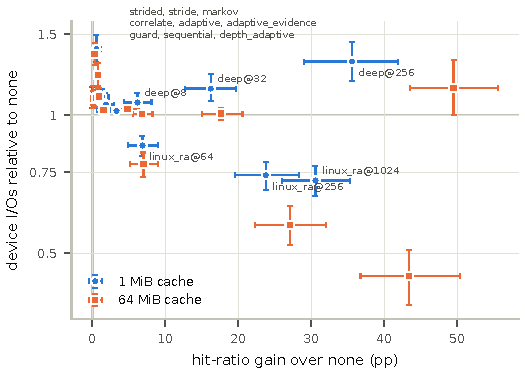
\includegraphics[width=\columnwidth]{figures/f3_device_io_vs_hit}
\caption{Simulated hit-ratio gain over \texttt{none} against device I/Os
relative to \texttt{none}, C1, both cache sizes, with paired \ciLevel{}
bootstrap intervals over the \diskTraces{} traces. Only window growth lies below
one.}
\label{fig:f3}
\end{figure}

\textbf{The learned class router.} The classifier-routed \texttt{adaptive}
policy is \decDiskPOneAdaptiveAssumedOneMiBVerdict{} than \texttt{sequential} at
both capacities (P1): \decDiskPOneAdaptiveAssumedOneMiBPairedCI{} paired and
\decDiskPOneAdaptiveAssumedOneMiBClusterCI{} cluster at 1\,MiB, losing on
\diskDeltaHitRatioAdaptiveVsSequentialOneMiBLosses{} of
\diskDeltaHitRatioAdaptiveVsSequentialOneMiBN{} traces, and
\decDiskPOneAdaptiveAssumedSixtyFourMiBPairedCI{} at 64\,MiB (losing on
\diskDeltaHitRatioAdaptiveVsSequentialSixtyFourMiBLosses). It still beats
\texttt{none} (\diskVsNoneAdaptiveOneMiBCI), but by less than the two-block
read-ahead it routes between, and with more device I/Os
(\diskIORatioAdaptiveOneMiB).

\textbf{The feedback gate.} Against \texttt{sequential}, \texttt{guard} is
\decDiskPTwoGuardAssumedSixtyFourMiBVerdict{} at 64\,MiB
(\decDiskPTwoGuardAssumedSixtyFourMiBPairedCI) and at 1\,MiB its result is
``\decDiskPTwoGuardAssumedOneMiBVerdict'' (paired
\decDiskPTwoGuardAssumedOneMiBPairedCI, cluster
\decDiskPTwoGuardAssumedOneMiBClusterCI). At the break-even cost model it is
\decDiskPTwoGuardBreakEvenOneMiBVerdict{} at both capacities and stays within
\diskBreakEvenVsNoneGuardOneMiB{} of \texttt{none}. The gate limits waste and device
work (\diskIORatioGuardOneMiB{} of \texttt{none}'s I/Os, against
\diskIORatioSequentialOneMiB{} for \texttt{sequential}) but adds no hits over
\texttt{sequential}. The gated mode that does add hits is
\texttt{depth\_adaptive}, which lets the same precision evidence also choose a
read-ahead depth: at the assumed cost model it is above \texttt{sequential} by
\diskDeltaHitRatioDepthAdaptiveVsSequentialOneMiBCI{} paired
(\diskDeltaHitRatioDepthAdaptiveVsSequentialOneMiBClusterCI{} cluster) at
1\,MiB and \diskDeltaHitRatioDepthAdaptiveVsSequentialSixtyFourMiBCI{} at
64\,MiB (exploratory: not a pre-registered comparison), and at the break-even
model it is identical to \texttt{guard}. Its gain comes with a choice of depth,
not with the gate alone.

\textbf{Which lever is smallest.} The pre-registered ordering compares the
intervals of $|\Delta|$ against \texttt{sequential}. At 1\,MiB the predictor
(\decDiskOneMiBPredictorSmallestPredictorPairedCI{} pp paired) and the
feedback gate (\decDiskOneMiBPredictorSmallestFeedbackPairedCI) cannot be
ordered; both are smaller than depth
(\decDiskOneMiBPredictorSmallestDepthPairedCI) and window growth
(\decDiskOneMiBPredictorSmallestWindowGrowthPairedCI), and depth is smaller than
window growth, in both the paired and the cluster intervals. At 64\,MiB the
order is complete: feedback, then the predictor, then depth, then window
growth. So the rule's verdict at both capacities is that
\decDiskSixtyFourMiBPredictorSmallestVerdict: the learned predictor moves the
hit ratio little, but the feedback gate moves it as little or less.

\textbf{Robustness.} Of the \decTallyCThree{} P1--P4 decisions that C3 repeats,
\decTallyCThreeRobust{} are \emph{robust} on a second slice of the subset traces;
\texttt{deep@32} against \texttt{none} is
\decDiskCThreeDeepAtThirtyTwoAssumedVerdict{} (better on the first slice,
paired-only on the second). On FIU, \decTallyCFourCapInsensitive{} of
\decTallyCFour{} are cap-insensitive between merge caps of 256 and 1024
sectors. Request reconstruction matters a great deal: on FIU at C2,
\texttt{deep@8} changes the hit ratio by
\diskDeltaFiuCTwoHitRatioDeepAtEightVsNoneOneMiBCI{} on merged requests (an
interval that contains zero) but by
\diskDeltaFiuCTwoNoneHitRatioDeepAtEightVsNoneOneMiBCI{} on the unmerged
4\,KiB page records, an artefact of counting each page as a request that we
report only as a sensitivity view.

\textbf{Learned depth and the LSTM.} The GPU-trained depth controller is
\decDiskLearnedDepthVsVcfCapTwoHundredFiftySixVerdict{} than the
validation-chosen fixed depth at both action caps, on held-out test segments:
\decDiskLearnedDepthVsVcfCapSixtyFourPairedCI{} with a 64-block cap (cluster
\decDiskLearnedDepthVsVcfCapSixtyFourClusterCI; it wins on
\ldVsVcfCapSixtyFourWins{} of \ldVsVcfCapSixtyFourN{} traces) and
\decDiskLearnedDepthVsVcfCapTwoHundredFiftySixPairedCI{} with a 256-block cap,
over \ldSeedsCapTwoHundredFiftySix{} seeds. The GPU study records prefetches,
not device I/Os: the controller issues \ldIssuedVsVcfCapSixtyFour{} and
\ldIssuedVsVcfCapTwoHundredFiftySix{} as many as VCF under the two caps. It does beat \texttt{deep@8}
(exploratory; \ldVsDeepEightCapTwoHundredFiftySixCI), but \texttt{deep@8} is not the fair
baseline: the depth a validation split chooses is. The LSTM predicts address deltas, so we compare only its
cache outcome: on its \lstmTraces{} traces its mean test hit ratio
(\lstmMeanHit) is below \texttt{linux\_ra}'s (\lstmMeanLinuxRaHit) on
\lstmBelowLinuxRa{} of \lstmTraces{} and close to \texttt{none}'s
(\lstmMeanNoneHit); its contended GPU timings are not quoted.
% <<< end sections/disk_results.tex
% >>> begin sections/realio_results.tex
% VII. Real-device validation (measured, E3). Every number is labelled
% measured with its device, backend and think model; prediction error and
% k_eff are stated per trace and think model, never as a property of HDDs
% or SSDs (constraint 15). The hard disk is the headline device; the SSD is
% secondary and a contended cell is not used (lead rulings).
% Sources: results/realio/{realio,realio_summary}.csv, device_*.json, via
% numbers.tex and paper/decisions.py. Generated: Table T3b, Fig. F5 (T3 in
% the appendix).

\section{Real-Device Validation (Measured)}\label{sec:realio}

% >>> begin tables/t3b_realio_summary.tex
% t3b_realio_summary.tex -- GENERATED by paper/tables/make_tables.py; do not edit.
% Inputs: realio/realio.csv, realio/realio_summary.csv
\begin{table*}[t]
\centering
\scriptsize
\setlength{\tabcolsep}{2pt}
\caption{Simulator against measurement (E3, measured) per device, backend, think model and 20{,}000-request trace prefix: Spearman rank correlation across modes of measured mean latency with simulated device time and with simulated hit ratio ($^{*}$: the pre-registered R2 rule finds a ranking consistent with measured latency, $^{\dagger}$: a ranking against it; unmarked: ranking not supported, or n = 4 and descriptive only), the mode with the lowest measured mean latency against the mode with the highest simulated hit ratio, and the mean error of the hit-ratio-only latency prediction. Stated per trace, not as a device property.}
\label{tab:t3b_realio_summary}
\begin{tabular}{llllrrrllrr}
\hline
Device & Backend & Think & Trace & Modes & $\rho$ dev.\ time & $\rho$ hit & Fastest & Max sim.\ hit & Pred.\ err.\ (\%) & Foreign (\%) \\
\hline
sdb & odirect & closed & alibabaBlock\_17 & 7/7 & $+0.61$ & $-0.46$ & linux\_ra & deep@64 & $-47.1$ & $0.00$ \\
sdb & odirect & closed & fiu\_homes-110108-112108 & 7/7 & $+0.86^{*}$ & $+0.21$ & none & deep@64 & $-30.1$ & $0.00$ \\
sdb & odirect & closed & msr\_hm\_0 & 7/7 & $-0.21$ & $+0.61$ & none & deep@64 & $-16.5$ & $0.00$ \\
sdb & odirect & closed & msr\_prn\_0 & 7/7 & $+0.46$ & $+0.61$ & none & deep@64 & $-36.6$ & $0.00$ \\
sdb & odirect & closed & msr\_web\_2 & 7/7 & $-0.23$ & $+0.13$ & deep@64 & linux\_ra & $-15.1$ & $0.00$ \\
sdb & pagecache & closed & alibabaBlock\_17 & 8/10 & $+0.24$ & $-0.50$ & kernel\_ra & deep@64 & $-35.6$ & $0.00$ \\
sdb & pagecache & closed & fiu\_homes-110108-112108 & 8/10 & $+0.98^{*}$ & $+0.17$ & kernel\_ra & deep@64 & $-35.4$ & $0.00$ \\
sdb & pagecache & closed & msr\_hm\_0 & 8/10 & $-0.18$ & $+0.61$ & none & deep@64 & $-14.0$ & $0.00$ \\
sdb & pagecache & closed & msr\_prn\_0 & 8/10 & $+0.64$ & $+0.57$ & none & deep@64 & $-23.5$ & $0.00$ \\
sdb & pagecache & closed & msr\_web\_2 & 8/10 & $-0.07$ & $-0.51$ & kernel\_seq & linux\_ra & $-16.8$ & $0.00$ \\
sdb & odirect & spread:1:5000 & msr\_hm\_0 & 7/7 & $-0.89^{\dagger}$ & $+0.75$ & guard & deep@64 & $-13.2$ & $0.00$ \\
sdb & pagecache & spread:1:5000 & msr\_hm\_0 & 8/10 & $+0.18$ & $-0.06$ & deep & deep@64 & $-16.1$ & $0.00$ \\
ssd & odirect & closed & msr\_hm\_0 & 4/4 & $+0.80$ & $-0.60$ & deep & linux\_ra & $-8.7$ & $0.20$ \\
ssd & odirect & closed & msr\_web\_2 & 4/4 & $+0.60$ & $+0.20$ & none & linux\_ra & $-26.4$ & $0.04$ \\
ssd & pagecache & closed & msr\_hm\_0 & 4/5 & $+0.60$ & $-0.80$ & kernel\_ra & linux\_ra & $-6.5$ & $0.18$ \\
ssd & pagecache & closed & msr\_web\_2 & 4/5 & $+0.20$ & $-1.00$ & contended & -- & $-19.9$ & $1.05$ \\
\hline
\end{tabular}
\\[2pt]{\scriptsize Modes: modes with a simulator plan / all modes in the cell (kernel\_ra and kernel\_seq have none). A cell whose foreign I/O exceeds 1\% is contended: no fastest mode is named and no rule is applied.}
\end{table*}
% <<< end tables/t3b_realio_summary.tex

The simulator assumes that prefetches complete instantly and cost the demand
stream nothing; the testbed measures what happens instead. All numbers here
are measured request latencies on the \realioRequests-request prefixes.
Backend~B's cache equalled the simulator's on every request of all
\realioOdirectRuns{} of its runs, so its differences come from timing alone.

\textbf{Prefetching was slower on the hard disk.} With Backend~B and a closed
loop on the hard disk, a prefetching mode \emph{raised} the mean latency
against \texttt{none} in \decCountROneSdbOdirectClosedRaises{} of
\decCountROneSdbOdirectClosed{} mode--trace cells, showed no difference
detectable with \realioReps{} repeats in
\decCountROneSdbOdirectClosedNoDifference, and lowered it in
\decCountROneSdbOdirectClosedLowers. On \texttt{msr\_hm\_0}, for example,
\texttt{deep@64} raises the simulated hit ratio from
\realioSimHitSdbOdirectNoneClosedMsrHmZero{} to
\realioSimHitSdbOdirectDeepAtSixtyFourClosedMsrHmZero{} and the measured mean
latency by \decRealioROneSdbOdirectClosedMsrHmZeroDeepAtSixtyFourCI. A plausible
cause is that the prefetches queue on the same spindle as the demand reads; a
prediction from the measured full-hit fraction alone misses this cell's mean
by \realioPredErrSdbOdirectDeepAtSixtyFourClosedMsrHmZero. Through the page cache
(Backend~A) the picture is mixed: \decCountROneSdbPagecacheClosedLowers{} of
\decCountROneSdbPagecacheClosed{} cells lower the mean, and
\decCountROneSdbPagecacheClosedRaises{} raise it.

\begin{figure*}[t]
\centering

\includegraphics[width=\textwidth]{figures/f5_sim_vs_measured}
\caption{Measured mean request latency against simulated hit ratio for every
mode with a simulator plan, per device and backend, closed loop (left) and
spread think time on \texttt{msr\_hm\_0} (right); bars are Student-$t$
intervals over \realioReps{} repeats. Higher simulated hit ratio does not mean
lower latency. Measured on one host; per trace, not a device property.}
\label{fig:f5}
\end{figure*}

\textbf{The simulator does not rank the modes.} By the pre-registered rank
rule, simulated hit ratio ranks the modes consistently with measured latency
in \decTallyRTwoHitRanksConsistentlyWithMeasuredLatency{} of the
\decTallyRTwoHit{} cells; the ranking is not supported in
\decTallyRTwoHitRankingNotSupported{}, where \decRhoPositiveHitSdb{} of the
\decRhoCellsHitSdb{} hard-disk correlations have the wrong (positive) sign, and
the SSD cells are too small for the test
(Table~\ref{tab:t3b_realio_summary}). Simulated device time, which charges
positioning per I/O, ranks consistently in
\decTallyRTwoDeviceTimeRanksConsistentlyWithMeasuredLatency{} cells (both on
the FIU trace) and against measured latency in
\decTallyRTwoDeviceTimeRanksAgainstMeasuredLatency. The mode with the highest
simulated hit ratio was the fastest in \decCellsTopSimFastest{} of the
\decCells{} uncontended cells, and \texttt{none} was the fastest in
\decCellsNoneFastest{} (Fig.~\ref{fig:f5}).

\textbf{The kernel's own read-ahead.} On Backend~A, the kernel's read-ahead
lowered the mean latency against \texttt{none} in
\decCountRSixSdbPagecacheClosedLowers{} of \decCountRSixSdbPagecacheClosed{}
cells: on \texttt{msr\_web\_2} the change was
\decRealioRSixSdbPagecacheClosedMsrWebTwoKernelRaCI{} for \texttt{kernel\_ra}
and \decRealioRSixSdbPagecacheClosedMsrWebTwoKernelSeqCI{} for
\texttt{kernel\_seq}. It raised it on
\texttt{msr\_prn\_0}
(\decRealioRSixSdbPagecacheClosedMsrPrnZeroKernelRaCI).

\textbf{Think time and the SSD.} Spreading each second's requests over that
second changed no mode's effect by the R7 rule
(\decTallyRSevenNoChangeByTheRSevenRule{} of \decTallyRSeven{} pairs; the spread
intervals are wide). On the SSD (secondary), Backend~B lowered the mean in
\decCountROneSsdOdirectClosedLowers{} of \decCountROneSsdOdirectClosed{} cells,
for instance \texttt{deep} on \texttt{msr\_hm\_0}
(\decRealioROneSsdOdirectClosedMsrHmZeroDeepCI), and raised it in
\decCountROneSsdOdirectClosedRaises; the page-cache cell of \texttt{msr\_web\_2}
exceeded the foreign-I/O limit and is not used.
% <<< end sections/realio_results.tex
% >>> begin sections/web_results.tex
% VIII. Web results (simulated, E4/E5). Object sizes, RTT and bandwidth are
% assumed and the cost c is an assumed number of hit-equivalents
% (constraint 8). Headline comparisons are against the best fixed depth at the
% same capacity, no prefetching and transition top-1 (constraint 7); nothing
% generalises from one capacity or one cost (web decision rule 1).
% Sources: results/web/{decomposition,comparisons,policy_metrics,freshness,
% seq_metrics,calibration}.csv, via numbers.tex and paper/decisions.py.
% Generated: Tables T5, T4, T6 and Fig. F6, all in the appendix (page budget).

\section{Web Results (Simulated)}\label{sec:web}

All numbers here replay the RetailRocket test split (\webSessions{} sessions)
through per-session caches with instant prefetch, with an assumed $c$.
Table~\ref{tab:t5_web_decomposition} in the appendix isolates one lever per
row against its pre-registered baseline.

\textbf{The controller.} Selected on validation separately at each capacity,
the adaptive controller (\polAdaptive) beats the best fixed depth at the same
capacity (W1; \decWebWOneCapEightCI{} in $U$ at $c$ = \webHeadlineCost{} and
capacity 8, \decWebWOneCapThirtyTwoCI{} at capacity 32), beats no prefetching
(W2; \decWebWTwoCapEightCI), and, in an exploratory comparison, beats
transition top-1 (\webCmpVsTransitionPerCapacityLogisticCapEightCostZeroPointZeroOneCI). By
decision rule 1 we may therefore say that \decWebRuleOneCapEightVerdict{} at
capacities 8 and 32, at this cost, and no more. It gets there by issuing less:
\webIssuedLogisticCapEightAdaptiveZeroPointZeroOne{} prefetches per view
against \webIssuedLogisticCapEightFixedOne{} for the best fixed depth, with a
hit ratio of \webHitLogisticCapEightAdaptiveZeroPointZeroOne{} against
\webHitLogisticCapEightFixedOne{} (\webHitLogisticCapEightFixedZero{} without
prefetching; every capacity and family is in Table~\ref{tab:t6_web_comparisons}).

\textbf{The ranker and its freshness.} The trained logistic ranker loses to
plain history: top-1 transition counts from the index split hit more often at
depth one (W3; \decWebWThreeHitRankerCI), although, as an
exploratory diagnostic, the logistic ranker is the better-calibrated of the
two (Brier skill \webBrierSkillLogistic{} against \webBrierSkillTransSZero{}
for the counts).
Counts updated online as the test split replays are worth far more (W4,
online counts minus the logistic ranker at depth four;
\decWebWFourHitFreshnessCI). Descriptively, the next item is in the online
index's top eight for \webCoverageOnlineKEight{} of eligible views, against
\webCoverageSplitZeroKEight{} for the shipped index (Fig.~\ref{fig:f6} in the
appendix).

\textbf{Depth.} Prefetching four items instead of one raises the hit ratio
(W5; \decWebWFiveHitDepthCI) but costs more than it gains at $c$ =
\webHeadlineCost{} (\decWebWFiveUtilityDepthCI{} in $U$): only
\webPrecisionLogisticCapEightFixedFour{} of its prefetches are used, against
\webPrecisionLogisticCapEightFixedOne{} at depth one. Depth is a lever in both
directions, which is consistent with a controller that chooses it per view
beating the validated best fixed depth.

\textbf{The feedback gate.} Against the adaptive controller, the validated
gate (\polFeedback) gets the verdict ``\decWebWSixHitFeedbackVerdict'' in hit
ratio (W6; \decWebWSixHitFeedbackCI) and ``\decWebWSixUtilityFeedbackVerdict''
in $U$ (\decWebWSixUtilityFeedbackCI), so by rule 3 it is
\decWebRuleThreeVerdict. It does issue fewer prefetches
(\webIssuedLogisticCapEightFeedbackZeroPointZeroOneEpsZeroPointZeroZeroFive{} per
view against \webIssuedLogisticCapEightAdaptiveZeroPointZeroOne).

\textbf{The sequence model.} The GRU, trained on the index and training splits
over \webSeqGruFinalCapEightFixedFourCostZeroPointZeroOneSeeds{} seeds, reaches
a hit ratio of \webSeqGruFinalCapEightFixedFourCostZeroPointZeroOneCacheHit{} at
depth four (seed range
\webSeqGruFinalCapEightFixedFourCostZeroPointZeroOneCacheHitMin{} to
\webSeqGruFinalCapEightFixedFourCostZeroPointZeroOneCacheHitMax), below the
online transition counts' \webHitTransOnlineCapEightFixedFour{} on every seed;
the pre-registered comparison (W8, seed 0) gives
``\decWebWEightHitSequenceModelVerdict'' (\decWebWEightHitSequenceModelCI).

\textbf{Scope and the lever rule.} One cache per visitor instead of per
session would add \decWebWSevenHitCacheScopeCI{} of hits with no prefetching
and an unbounded cache (W7); this is an upper bound on cross-session reuse,
not a prefetching result. By rule 2, the ranker lever
($|\Delta|$ in \decWebPredictorSmallestRankerCI{} pp) is smaller than both
depth (\decWebPredictorSmallestDepthCI) and freshness
(\decWebPredictorSmallestFreshnessCI), but the sequence-model lever
(\decWebPredictorSmallestSequenceModelCI) overlaps depth, so
\decWebPredictorSmallestVerdict{} and we make no ordering claim between the
sequence model and depth.
% <<< end sections/web_results.tex
% >>> begin sections/live_results.tex
% IX. Live HTTP results (measured on loopback with an emulated network;
% RTT, bandwidth and object sizes are ASSUMED; constraint 8). Only valid
% passes are cited, and SSD-store passes with more than 1 % foreign I/O are
% left out (lead ruling; genlib.live_citable).
% Sources: results/live/{live_metrics,live_parity}.csv, live_config.json,
% via numbers.tex and paper/decisions.py. Generated: Table T7 (T7b and
% Fig. F7 in the appendix).

\section{Live HTTP Results (Measured)}\label{sec:live}

% >>> begin tables/t7_live.tex
% t7_live.tex -- GENERATED by paper/tables/make_tables.py; do not edit.
% Inputs: live/live_metrics.csv, live/live_parity.csv
\begin{table*}[t]
\centering
\footnotesize
\setlength{\tabcolsep}{3pt}
\caption{Live HTTP replay (measured on loopback with an emulated network; RTT, bandwidth and object sizes are ASSUMED). Milliseconds of wait saved per view against the no-prefetch baseline: mean over citable passes (valid, and at most 1\% foreign I/O on the store device), with the envelope of the per-pass 95\% session-bootstrap CIs. Parity: sessions whose live counters differ from the simulator's.}
\label{tab:t7_live}
\begin{tabular}{llrrrrrrrr}
\hline
Store & Policy & Passes & Hit (\%) & Wait (ms) & Saved (ms) & Ideal saved & Wasted KiB & Bytes & Parity \\
\hline
\multicolumn{10}{l}{\emph{hdd object store}} \\
\hline
hdd & adaptive\_0.01 & 3 & $27.3$ & $109.1$ & $4.98$ {\scriptsize [$4.14$, $5.89$]} & $3.19$ & $94.6$ & $2.19\times$ & 0 \\
hdd & adaptive\_0.1@trans\_online & 3 & $29.2$ & $105.8$ & $8.27$ {\scriptsize [$7.09$, $9.73$]} & $6.12$ & $95.4$ & $2.20\times$ & 0 \\
hdd & feedback\_0.01\_eps0.005 & 3 & $27.9$ & $107.1$ & $6.99$ {\scriptsize [$5.95$, $8.19$]} & $4.34$ & $159.4$ & $3.00\times$ & 0 \\
hdd & fixed0 & 3 & $24.9$ & $114.1$ & $0.00$ {\scriptsize [$0.00$, $0.00$]} & $0.00$ & $0.0$ & $1.00\times$ & 0 \\
hdd & fixed4 & 3 & $28.4$ & $105.9$ & $8.18$ {\scriptsize [$6.91$, $9.71$]} & $5.09$ & $455.0$ & $6.71\times$ & 0 \\
hdd & fixed8 & 3 & $27.4$ & $106.9$ & $7.23$ {\scriptsize [$6.33$, $8.14$]} & $3.32$ & $1108.8$ & $14.91\times$ & 0 \\
\hline
\multicolumn{10}{l}{\emph{ssd object store}} \\
\hline
ssd & adaptive\_0.01 & 1 & $27.3$ & $101.8$ & $3.39$ {\scriptsize [$2.75$, $4.13$]} & $3.19$ & $94.6$ & $2.19\times$ & 0 \\
ssd & adaptive\_0.1@trans\_online & 2 & $29.2$ & $98.8$ & $6.36$ {\scriptsize [$5.34$, $7.51$]} & $6.12$ & $95.4$ & $2.20\times$ & 0 \\
ssd & feedback\_0.01\_eps0.005 & 2 & $27.9$ & $100.6$ & $4.58$ {\scriptsize [$3.72$, $5.67$]} & $4.34$ & $159.4$ & $3.00\times$ & 0 \\
ssd & fixed0 & 3 & $24.9$ & $105.2$ & $0.00$ {\scriptsize [$0.00$, $0.00$]} & $0.00$ & $0.0$ & $1.00\times$ & 0 \\
ssd & fixed4 & 3 & $28.4$ & $99.8$ & $5.40$ {\scriptsize [$4.45$, $6.53$]} & $5.09$ & $455.0$ & $6.71\times$ & 0 \\
ssd & fixed8 & 2 & $27.4$ & $101.8$ & $3.39$ {\scriptsize [$2.64$, $4.14$]} & $3.32$ & $1108.8$ & $14.91\times$ & 0 \\
\hline
\end{tabular}
\\[2pt]{\scriptsize 0 headline pass-policy row(s) failed the validity gate and 5 valid row(s) carried more than 1\% foreign I/O on the store device; both are excluded.}
\end{table*}
% <<< end tables/t7_live.tex

Every saving here is measured on loopback with an emulated \liveRttMs{} round
trip, a \liveMbps{} link and assumed object sizes; it is not a page-load
speedup of a real site. All \liveRows{} pass--policy rows passed the validity
gate, with \liveParityMismatches{} sessions whose live counters differ from the
simulator's (H1); \liveFlaggedRows{} SSD-store rows had over one percent foreign
I/O and are not cited.

\textbf{Prefetching lowered the wait.} With the hard-disk object store, all
\decTallyHTwoHddLowersTheMeanWait{} prefetching policies lowered the mean wait
against no prefetching in every repetition (H2; Table~\ref{tab:t7_live}). The
online-index controller (\polOnline) saved
\liveSavedHddAdaptiveZeroPointOneAtTransOnlineCI{} per view and \texttt{fixed4}
\liveSavedHddFixedFourCI, against a no-prefetch wait of \liveBaseWaitHdd; the
bracket is the envelope of the per-repetition session-bootstrap intervals. On
the SSD store \decTallyHTwoSsdLowersTheMeanWait{} of \decTallyHTwoSsd{}
policies lowered the wait; for \polAdaptive{} the effect is
\decLiveHTwoSsdAdaptiveZeroPointZeroOneVerdict, because only
\liveRepsSsdAdaptiveZeroPointZeroOne{} of its \liveHeadlineReps{} repetitions was
unflagged.

\textbf{The instant-prefetch model understated the hard-disk benefit.} The
model-ideal wait is zero on a hit and the round trip plus transfer on a miss.
On the hard-disk store the measured saving exceeded the model-ideal saving for
all \decTallyHThreeHddTheInstantPrefetchModelUnderstatesTheBenefit{} policies
(H3): \texttt{fixed8} saved \liveSavedHddFixedEight{} against a model-ideal
\liveIdealSavedHddFixedEight. The ideal model has no disk; a plausible reason is that
every demand miss on the hard disk also waits for a seek, which a prefetched
object avoids. On
the SSD store all \decTallyHThreeSsdConsistentWithTheModel{} policies were
consistent with the model, and the store changed the saving for
\decTallyHSevenTheStoreChangesTheDelta{} of \decTallyHSeven{} policies (H7).

\textbf{Bytes, scheduling and hints.} The savings cost bandwidth:
\texttt{fixed8} transferred \liveBytesXHddFixedEight{} the bytes of no
prefetching and saved less than \texttt{fixed4}; the two validated adaptive
controllers moved \liveBytesXHddAdaptiveZeroPointZeroOne{} and
\liveBytesXHddAdaptiveZeroPointOneAtTransOnline, and they are the only policies
no other policy beats on both saved wait and bytes (H4, descriptive;
Fig.~\ref{fig:f7}). Demand priority on the link matters for deep prefetching:
under a FIFO link, \texttt{fixed8}'s change in wait was
\decLiveHFiveSsdFixedEightFIFOCI, against \decLiveHFiveSsdFixedEightPriorityRepOneCI{}
with priority, so \decLiveHFiveSsdFixedEightVerdict{} (H5); for \texttt{fixed4}
there was \decLiveHFiveSsdFixedFourVerdict. Server-side read-ahead hints alone,
with no client prefetch, lowered the wait in one repetition on the hard disk
(H6; \decLiveHSixHddHintFixedEightCI{} for eight hinted objects).
% <<< end sections/live_results.tex
% >>> begin sections/classifier_results.tex
% X. The classifier study (simulated). Three follow-up experiments, each
% pre-registered after E1-E6 were known (results/{classifier,hindsight,
% web_rankers}/PREREGISTERED.md): the classifier zoo and the real-trace
% router benchmark (track CLF), the hindsight-labelled router whose actions
% include read-ahead depth (HSR), and the web ranker alternatives (WRK); the
% MSRC light sample (E7) is in the appendix. Every verdict is a \dec macro
% computed by paper/decisions.py; synthetic accuracies are labelled
% synthetic; every disk hit ratio is paired with device work.
% Generated: Fig. F9 (Tables T10-T13 in the appendix).

\section{Can a Better Learner Help? (Simulated)}\label{sec:classifiers}

The disk router of Section~\ref{sec:disk} uses Gaussian naive
Bayes~\cite{domingos1997optimality,zhang2004optimality} to put each 32-request
window in one of four classes, and each class prefetches at most two blocks,
so even a perfect classifier can do little better than \texttt{sequential}. We
tested that bound three ways, under rules committed after E1--E6 were known
(so not blind to them): replace the classifier, give a router read-ahead depth
as an action, and replace the web ranker.

\textbf{Methods.} Besides the shipped online GNB and QDA we tuned
\clfSynTunedFamilies{} scikit-learn families~\cite{pedregosa2011sklearn}, from
discriminant analysis and logistic regression to $k$NN, SVMs, CART, forests,
boosting and an MLP (the list with its citations is in the appendix), each
with \clfSynCandidates{} random-search candidates~\cite{bergstra2012random}
chosen on training seeds alone; test seeds were scored once. The fitted
models then routed \texttt{adaptive} unchanged on C3's second slice of
\clfRouterTraces{} traces. On synthetic windows (appendix,
Table~\ref{tab:t10_classifier_zoo}) the tree models and boosting match GNB
under the block-size shift that made us keep it, and beat it on heavy phase
blends, an optimistic synthetic margin.

\begin{figure}[t]
\centering
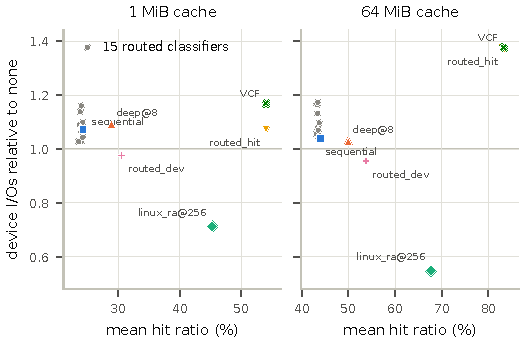
\includegraphics[width=\columnwidth]{figures/f9_action_space}
\caption{The action-space ceiling (simulated, C3 slice 2, \clfRouterTraces{}
traces): mean hit ratio against device I/Os relative to \texttt{none}. The
\clfRouterClassifiers{} routed classifiers sit with \texttt{sequential};
depth, window growth and the hindsight routers move away from it. VCF is the
validation-chosen fixed action.}
\label{fig:f9}
\end{figure}

\textbf{Routing real traces} (Fig.~\ref{fig:f9},
Table~\ref{tab:t11_classifier_router}). By the claim rule,
\decClfClaimBeatsReadAheadOneMiBVerdict{} at either capacity: all
\decTallyClfOneOneMiB{} show no difference detected against
\texttt{sequential} at 1\,MiB and all are worse at 64\,MiB (the best, an MLP,
by \decClfOneMlpSixtyFourMiBPairedCI). Against the shipped GNB, only the random
forest is better at 1\,MiB (\decClfTwoRfOneMiBPairedCI{} paired,
\decClfTwoRfOneMiBClusterCI{} cluster), and \decTallyClfTwoSixtyFourMiBBetter{}
of \decTallyClfTwoSixtyFourMiB{} alternatives are at 64\,MiB. Every routed
classifier increases device I/Os (\clfRouterIORatioMinOneMiB--\clfRouterIORatioMaxOneMiB{}
of \texttt{none}'s at 1\,MiB), while \texttt{linux\_ra@256} adds
\decClfOneLinuxRaAtTwoHundredFiftySixOneMiBPaired{} over \texttt{sequential}
with \clfRouterIORatioLinuxRaAtTwoHundredFiftySixOneMiB{} of the I/Os. The
classifiers agree with GNB on only \clfRouterAgreementMin--\clfRouterAgreementMax{}
of windows, yet the hit ratio barely moves: the class decides little when
every class prefetches two blocks at most.

\textbf{Depth as an action.} The hindsight router picks the next window's
action among \texttt{none}, \texttt{sequential}, \texttt{deep@8},
\texttt{deep@32} and \texttt{deep@256}. Its label is the action that did best
on that window in its own fixed replay, a trajectory approximation in the
spirit of hindsight-labelled caching~\cite{jain2016hawkeye} and open to the
distribution shift of imitation learning~\cite{ross2011reduction}. We selected
among \hsrCvFamilies{} families by corpus-grouped cross-validation on the
first slice and scored the second (Table~\ref{tab:t12_hindsight}). Against the
per-trace validation-chosen fixed action (VCF), the router shows
\decHsrHOneHitRatioRoutedHitVsVcfHitOneMiBVerdict{} at 1\,MiB
(\decHsrHOneHitRatioRoutedHitVsVcfHitOneMiBPairedCI) and is
\decHsrHOneHitRatioRoutedHitVsVcfHitSixtyFourMiBVerdict, by a negligible
\decHsrHOneHitRatioRoutedHitVsVcfHitSixtyFourMiBPaired, at 64\,MiB, where it
sends \hsrDeepShareRoutedHitSixtyFourMiB{} of windows to \texttt{deep@256}, the
VCF action. Its gains over \texttt{sequential}
(\decHsrHTwoHitRatioRoutedHitVsSequentialOneMiBPaired{} at 1\,MiB) and
\texttt{linux\_ra@256} are depth's, at \hsrMovedRatioRoutedHitOneMiB{} the
blocks moved by \texttt{none}. A device-objective router
\decHsrDDeviceIosRoutedDevVsNoneOneMiBVerdict{}
(\decHsrDDeviceIosRoutedDevVsNoneOneMiBPaired{} of \texttt{none}'s), but
\texttt{linux\_ra@256} needs only \hsrIORatioLinuxRaAtTwoHundredFiftySixOneMiB.
GNB had the lowest cross-validation score in \hsrCvGnbLowest{} of
\hsrCvCells{} cells, yet the best family does not beat VCF; nor is the
trajectory oracle a true ceiling, since it beats VCF at 1\,MiB only.

\textbf{Web rankers} (Table~\ref{tab:t13_web_rankers}). On the same candidates
and features, tuned boosting, forests, extra trees and an MLP rank better than
the shipped logistic ranker (MLP: \decWrkKOneMlpMrrAtEightCI{} in MRR@8). By the
primary rule, \decWrkRuleTwoCapEightVerdict{} at both capacities, the one
learned predictor here that does: the validation-selected MLP raises $U(c)$ per
view at $c$ = \webHeadlineCost{} by \decWrkSOneMlpUtilityPerViewCapEightCI{} at
capacity 8 and \decWrkSOneMlpUtilityPerViewCapThirtyTwoCI{} at 32, though its
hit ratio at capacity 8 is lower (\decWrkSOneMlpHitRatioCapEightCI). No family
beats transition top-1 at depth 1, and all stay far below online counts (MLP:
\decWrkKFiveMlpHitRatioCapEightCI): a better ranker does not close the
freshness gap.
% <<< end sections/classifier_results.tex
% >>> begin sections/discussion.tex
% X. Cross-domain discussion. States how the pre-registered hypothesis came
% out, from the decision rules of each results/*/PREREGISTERED.md
% (paper/decisions.py). Does not generalise from one trace, capacity or cost
% (constraint 7). Generated: Fig. F8 (Table T8 in the appendix).

\section{Cross-Domain Discussion}\label{sec:discussion}

\begin{figure*}[t]
\centering

\includegraphics[width=\textwidth]{figures/f8_utility_envelopes}
\caption{Simulated utility $U(c)$ of every policy (grey) and its upper envelope
(coloured by the winning policy) against the cost of one prefetch. Left: disk,
C1, 1\,MiB, means over \diskEnvelopeTracesOneMiB{} paired traces, with the two cost
models marked. Right: web test split, logistic ranker, capacity 8, with the
assumed costs marked. The envelope is computed in hindsight on the test data
and is not a selection.}
\label{fig:f8}
\end{figure*}

\textbf{One objective, two domains.} Fig.~\ref{fig:f8} puts both domains on
the axis of Eq.~\eqref{eq:utility}. On disk, the deepest read-ahead
(\diskEnvelopeBestZeroOneMiB) is best when a prefetch is free, window growth
(\diskEnvelopeBestAssumedOneMiB) at the assumed cost model's $c$, and no
prefetching at the break-even model's $c$ above one. On the web, the best
policy at every marked positive cost is an adaptive controller that chooses
its depth per view (\webEnvelopeBestCostZeroPointZeroOne{} at $c$ =
\webHeadlineCost, \webEnvelopeBestCostZeroPointTwoFive{} at the largest marked
cost). In both domains the policy that wins changes with the price of a
prefetch, and it is a choice of how much to fetch.

\textbf{The hypothesis, by its rules.} The pre-registered hypothesis had three
parts. \emph{The predictor is the smallest lever:} not established in either
study. No learned predictor beat its simple, fair baseline (the class
router lost to \texttt{sequential}, the depth network to the validation-chosen
depth, the logistic ranker to transition counts, the GRU to online counts),
but on disk the feedback gate moved the hit ratio as little or less, and on
the web the GRU's loss could not be separated from the depth lever's gain.
\emph{Depth and freshness are large levers:} supported by the orderings. On
disk, depth and window growth are larger than both the predictor and the gate
at both cache sizes; on the web, freshness is larger than the ranker. \emph{Feedback is a large lever:} not supported. The disk
gate is no better than \texttt{sequential} and the web gate shows no
detectable difference from the adaptive controller; both mainly issue less.
The one gated disk mode above \texttt{sequential}, \texttt{depth\_adaptive},
also chooses its depth (an exploratory comparison).

\textbf{Is the learner the problem?} No, in either domain. On disk, any of
\clfRouterClassifiers{} classifiers leaves the router level with or below
\texttt{sequential}, because its actions prefetch two blocks at most; with
depth as an action a router only reaches a fixed depth chosen per trace,
moving \hsrMovedRatioRoutedHitOneMiB{} the blocks of no prefetching at 1\,MiB.
On the web a better ranker helps the controller slightly, but transition
top-1 and online counts stay ahead. A learner matters only once its decision
can move the result, and even then depth and freshness decide more.

\textbf{Simulation against measurement.} The two real-system studies point in
opposite directions, and both are measured. On a hard disk with O\_DIRECT and
a closed loop, the simulator's higher hit ratio turned into higher latency in
most cells,
plausibly because prefetch reads compete with demand reads for one device.
Over HTTP, the link serves demand first, a prefetched object skips both the
round trip and the disk, and the instant-prefetch model \emph{understated}
the saving on the hard-disk store.
The simulator's hit ratio is therefore a statement about the cache, not about
latency, and which way the error goes depends on where the bottleneck sits.

\textbf{For a system designer.} Choose how much to prefetch per workload and
per price of a prefetch, prefer window growth that merges reads when device
operations are the cost, keep the statistics fresh, and validate on the real
device before trusting a simulated hit ratio. A learned predictor must beat
these baselines on held-out data to earn its training cost; none of ours did,
tuned or not.
% <<< end sections/discussion.tex
% >>> begin sections/threats.tex
% XI. Threats to validity. The long form of each item is in the plan
% (MASTER_PLAN section 5) and the pre-registrations; this is the summary.

\section{Threats to Validity}\label{sec:threats}

\textbf{Trace format.} The oracleGeneral records carry no read/write flag and
no service time, and their timestamps are whole seconds; writes are replayed
as reads, and think time on the real device is reconstructed from those
seconds. The FIU page-merge rule is our reconstruction; the sensitivity rows
show that leaving pages unmerged would change the FIU depth gain drastically.
The disk study replays a prefix of each trace (C3 checks a second slice), and
near-duplicate traces are down-weighted only in the cluster bootstrap.

\textbf{Model assumptions.} Both simulators assume a prefetch completes
instantly; the real-device and live studies measure what that assumption
hides, but only on \realioTraces{} trace prefixes and one web sample. The
simulators use LRU while the kernel uses its multi-generational LRU, which is
why Backend~A's hit ratio is reported as a divergence. Web object sizes, the
round-trip time and the bandwidth are assumed, the cache is per session,
sessions are cut by a fixed gap, and all web data come from one retailer.


\textbf{Statistics.} No correction for multiple comparisons is applied; we
state only the pre-registered comparisons as findings and label the rest
exploratory. The real-device intervals rest on \realioReps{} repeats and are
wide. The learned-depth comparison had no pre-registration of its own and is
read with the disk rule. Trained artifacts are scored only on data they were
not trained or selected on.

\textbf{The classifier study} was pre-registered after E1--E6 were known.
Its synthetic accuracies favour the phase blends (a window's context comes from
earlier windows of its class) and are never real-trace accuracies; the
hindsight labels approximate the counterfactual by each action's own
trajectory, and its search was cut by a dated amendment; prediction times were
contended; the MSRC check uses seven size-selected files whose flag tracks
address contiguity.

\textbf{Environment.} The host and GPU were shared; load and foreign I/O were
recorded for every run, contended cells and flagged passes are excluded, and
no GPU time is quoted as a cost. Each real-device result holds for its trace,
think model and device, not for hard disks or SSDs in general.
% <<< end sections/threats.tex
% >>> begin sections/conclusion.tex
% XII. Conclusion and future work. Restates only results already given,
% through the same numbers.tex macros.

\section{Conclusion and Future Work}\label{sec:conclusion}

Across \diskTraces{} block traces and the RetailRocket sessions, under rules
fixed before the experiments ran, the decisions that moved prefetching were
how much to fetch and how fresh the statistics were. Window growth gained
\decDiskPFourLinuxRaAtTwoHundredFiftySixAssumedOneMiBPaired{} of simulated hit
ratio while reducing device I/Os, and online counts gained
\decWebWFourHitFreshnessCI{} on the web. No learned predictor we trained beat
its simple baseline, and the pre-registered feedback gates limited waste
without adding hits; the one gated mode that did add hits also chose depth. Tuning or replacing the
classifier did not change this: the router's actions, not its learner, cap
its gain, and a router given depth as an action only matched a fixed depth
chosen per trace. On a real hard disk the simulated gains did not become lower latency
in most O\_DIRECT cells, while over emulated HTTP with a hard-disk store the
measured savings exceeded the model's. Future work should
test learned \emph{depth} and admission against window growth on the real
device rather than in simulation, measure the web cost $c$ instead of assuming
it, and repeat the live study on a real network.
% <<< end sections/conclusion.tex

% (bibliography style: IEEE, formatted by flatten.py below)
% Bibliography: formatted by paper/flatten.py from refs.bib, cited keys only,
% numbered in order of first citation (IEEEtran's unsorted order). It
% replaces \bibliographystyle{IEEEtran} and \bibliography{refs}, so this file
% needs neither BibTeX nor refs.bib.
\begin{thebibliography}{99}
\bibitem{wu2007readahead}
F.~Wu, H.~Xi, J.~Li, and N.~Zou, ``Linux Readahead: Less Tricks for More,'' in \emph{Proceedings of the Linux Symposium (OLS 2007)}, vol.~2. Ottawa, Canada, 2007, pp.~273--284. [Online]. Available: \url{https://www.kernel.org/doc/ols/2007/ols2007v2-pages-273-284.pdf}

\bibitem{linux_mmapi_readahead}
{The Linux Kernel Documentation}, ``Memory Management {APIs}: Readahead,'' \url{https://www.kernel.org/doc/html/latest/core-api/mm-api.html}, 2026. Kernel-doc generated from mm/readahead.c. Accessed 2026-10-26.

\bibitem{gill2005sarc}
B.~S.~Gill and D.~S.~Modha, ``{SARC}: Sequential Prefetching in Adaptive Replacement Cache,'' in \emph{Proceedings of the 2005 USENIX Annual Technical Conference, General Track}. USENIX Association, 2005, pp.~293--308.

\bibitem{gill2007amp}
B.~S.~Gill and L.~A.~D.~Bathen, ``{AMP}: Adaptive Multi-stream Prefetching in a Shared Cache,'' in \emph{5th USENIX Conference on File and Storage Technologies (FAST 07)}. San Jose, CA: USENIX Association, 2007, pp.~185--198. [Online]. Available: \url{https://www.usenix.org/conference/fast-07/amp-adaptive-multi-stream-prefetching-shared-cache}

\bibitem{padmanabhan1996using}
V.~N.~Padmanabhan and J.~C.~Mogul, ``Using Predictive Prefetching to Improve {World Wide Web} Latency,'' \emph{ACM SIGCOMM Computer Communication Review}, vol.~26, no.~3, pp.~22--36, 1996. doi: 10.1145/235160.235164.

\bibitem{fan1999web}
L.~Fan, P.~Cao, W.~Lin, and Q.~Jacobson, ``Web Prefetching between Low-Bandwidth Clients and Proxies: Potential and Performance,'' in \emph{Proceedings of the 1999 ACM SIGMETRICS International Conference on Measurement and Modeling of Computer Systems}. ACM, 1999, pp.~178--187. doi: 10.1145/301453.301557.

\bibitem{chakraborttii2020learning}
C.~Chakraborttii and H.~Litz, ``Learning {I/O} Access Patterns to Improve Prefetching in {SSDs},'' in \emph{Machine Learning and Knowledge Discovery in Databases: Applied Data Science Track (ECML PKDD 2020), Part IV}, ser. Lecture Notes in Computer Science, vol.~12460. Springer, 2021, pp.~427--443. doi: 10.1007/978-3-030-67667-4\_26.

\bibitem{hashemi2018learning}
M.~Hashemi, K.~Swersky, J.~Smith, G.~Ayers, H.~Litz, J.~Chang, C.~Kozyrakis, and P.~Ranganathan, ``Learning Memory Access Patterns,'' in \emph{Proceedings of the 35th International Conference on Machine Learning (ICML)}, ser. Proceedings of Machine Learning Research, vol.~80. PMLR, 2018, pp.~1919--1928. [Online]. Available: \url{https://proceedings.mlr.press/v80/hashemi18a.html}

\bibitem{wong2024baleen}
D.~L.-K.~Wong, H.~Wu, C.~Molder, S.~Gunasekar, J.~Lu, S.~Khandkar, A.~Sharma, D.~S.~Berger, N.~Beckmann, and G.~R.~Ganger, ``Baleen: {ML} Admission \& Prefetching for Flash Caches,'' in \emph{22nd USENIX Conference on File and Storage Technologies (FAST 24)}. Santa Clara, CA: USENIX Association, 2024, pp.~347--371. [Online]. Available: \url{https://www.usenix.org/conference/fast24/presentation/wong}

\bibitem{savva2026adaptive}
G.~Savva and H.~Herodotou, ``Adaptive Data Prefetching for File Storage Systems Using Online Machine Learning,'' \emph{Big Data and Cognitive Computing}, vol.~10, no.~1, p.~28, 2026. doi: 10.3390/bdcc10010028.

\bibitem{hidasi2016session}
B.~Hidasi, A.~Karatzoglou, L.~Baltrunas, and D.~Tikk, ``Session-based Recommendations with Recurrent Neural Networks,'' in \emph{4th International Conference on Learning Representations (ICLR 2016)}, 2016. arXiv:1511.06939. [Online]. Available: \url{https://arxiv.org/abs/1511.06939}

\bibitem{wu2010concurrent}
F.-G.~Wu, H.-S.~Xi, and C.-F.~Xu, ``File Prefetching Algorithm for Concurrent Streams,'' \emph{Journal of Software}, vol.~21, no.~8, pp.~1820--1833, 2010. doi: 10.3724/SP.J.1001.2010.03605.

\bibitem{man_posix_fadvise}
{Linux man-pages project}, ``posix\_fadvise(2): Predeclare an Access Pattern for File Data,'' \url{https://man7.org/linux/man-pages/man2/posix_fadvise.2.html}, 2026. Linux man-pages 6.19, page dated 2026-02-08. Covers POSIX\_FADV\_WILLNEED and POSIX\_FADV\_DONTNEED. Accessed 2026-10-26.

\bibitem{man_readahead}
{Linux man-pages project}, ``readahead(2): Initiate File Readahead into Page Cache,'' \url{https://man7.org/linux/man-pages/man2/readahead.2.html}, 2026. Linux man-pages 6.19, page dated 2026-02-08. Linux-specific; added in Linux 2.4.13. Accessed 2026-10-26.

\bibitem{ding2007diskseen}
X.~Ding, S.~Jiang, F.~Chen, K.~Davis, and X.~Zhang, ``{DiskSeen}: Exploiting Disk Layout and Access History to Enhance {I/O} Prefetch,'' in \emph{Proceedings of the 2007 USENIX Annual Technical Conference}. Santa Clara, CA: USENIX Association, 2007, pp.~261--274. [Online]. Available: \url{https://www.usenix.org/events/usenix07/tech/ding.html}

\bibitem{li2004cminer}
Z.~Li, Z.~Chen, S.~M.~Srinivasan, and Y.~Zhou, ``{C-Miner}: Mining Block Correlations in Storage Systems,'' in \emph{3rd USENIX Conference on File and Storage Technologies (FAST 04)}. San Francisco, CA: USENIX Association, 2004. [Online]. Available: \url{https://www.usenix.org/conference/fast-04/c-miner-mining-block-correlations-storage-systems}

\bibitem{soundararajan2008context}
G.~Soundararajan, M.~Mihailescu, and C.~Amza, ``Context-Aware Prefetching at the Storage Server,'' in \emph{2008 USENIX Annual Technical Conference (USENIX ATC 08)}. Boston, MA: USENIX Association, 2008. [Online]. Available: \url{https://www.usenix.org/conference/2008-usenix-annual-technical-conference/context-aware-prefetching-storage-server}

\bibitem{patterson1995informed}
R.~H.~Patterson, G.~A.~Gibson, E.~Ginting, D.~Stodolsky, and J.~Zelenka, ``Informed Prefetching and Caching,'' in \emph{Proceedings of the Fifteenth ACM Symposium on Operating Systems Principles (SOSP '95)}. ACM, 1995, pp.~79--95. doi: 10.1145/224056.224064.

\bibitem{cao1995integrated}
P.~Cao, E.~W.~Felten, A.~R.~Karlin, and K.~Li, ``A Study of Integrated Prefetching and Caching Strategies,'' in \emph{Proceedings of the 1995 ACM SIGMETRICS Joint International Conference on Measurement and Modeling of Computer Systems}. ACM, 1995, pp.~188--197. doi: 10.1145/223587.223608.

\bibitem{griffioen1994reducing}
J.~Griffioen and R.~Appleton, ``Reducing File System Latency using a Predictive Approach,'' in \emph{Proceedings of the USENIX Summer 1994 Technical Conference}. Boston, MA: USENIX Association, 1994. [Online]. Available: \url{https://www.usenix.org/conference/usenix-summer-1994-technical-conference/reducing-file-system-latency-using-predictive}

\bibitem{kroeger2001design}
T.~M.~Kroeger and D.~D.~E.~Long, ``Design and Implementation of a Predictive File Prefetching Algorithm,'' in \emph{Proceedings of the 2001 USENIX Annual Technical Conference}. Boston, MA: USENIX Association, 2001, pp.~105--118. [Online]. Available: \url{https://www.usenix.org/conference/2001-usenix-annual-technical-conference/design-and-implementation-predictive-file}

\bibitem{joseph1997markov}
D.~Joseph and D.~Grunwald, ``Prefetching using {Markov} Predictors,'' in \emph{Proceedings of the 24th Annual International Symposium on Computer Architecture (ISCA '97)}. ACM, 1997, pp.~252--263. doi: 10.1145/264107.264207.

\bibitem{hochreiter1997lstm}
S.~Hochreiter and J.~Schmidhuber, ``Long Short-Term Memory,'' \emph{Neural Computation}, vol.~9, no.~8, pp.~1735--1780, 1997. doi: 10.1162/neco.1997.9.8.1735.

\bibitem{chakraborttii2022deep}
C.~Chakraborttii and H.~Litz, ``Deep Learning-based Prefetching for Flash,'' in \emph{Non-Volatile Memories Workshop (NVMW)}, 2022. Workshop abstract; NSF PAR record 10332957. [Online]. Available: \url{https://par.nsf.gov/biblio/10332957}

\bibitem{lucasfilho2023streaming}
E.~R.~{Lucas Filho}, L.~Yang, K.~Fu, and H.~Herodotou, ``Streaming Machine Learning for Supporting Data Prefetching in Modern Data Storage Systems,'' in \emph{Proceedings of the First Workshop on AI for Systems (AI4Sys '23)}. ACM, 2023, pp.~7--12. doi: 10.1145/3588982.3603608.

\bibitem{ramadhan2026capsule}
A.~R.~Ramadhan, S.~Yoo, and J.~Choi, ``{CAPSULE}: A Storage Prefetcher Harnessing Spatio-Temporal Locality for Cloud-Scale Workloads,'' \emph{ACM SIGMETRICS Performance Evaluation Review}, vol.~54, no.~1, pp.~76--78, 2026. doi: 10.1145/3820171.3806897.

\bibitem{akgun2021kml}
I.~U.~Akgun, A.~S.~Aydin, A.~Shaikh, L.~Velikov, and E.~Zadok, ``A Machine Learning Framework to Improve Storage System Performance,'' in \emph{Proceedings of the 13th ACM Workshop on Hot Topics in Storage and File Systems (HotStorage '21)}. ACM, 2021, pp.~94--102. doi: 10.1145/3465332.3470875.

\bibitem{garg2024crossprefetch}
S.~Garg, J.~Zhang, R.~Pitchumani, M.~Parashar, B.~Xie, and S.~Kannan, ``{CrossPrefetch}: Accelerating {I/O} Prefetching for Modern Storage,'' in \emph{Proceedings of the 29th ACM International Conference on Architectural Support for Programming Languages and Operating Systems, Volume 1 (ASPLOS '24)}. ACM, 2024, pp.~102--116. doi: 10.1145/3617232.3624872.

\bibitem{maruf2020leap}
H.~{Al Maruf} and M.~Chowdhury, ``Effectively Prefetching Remote Memory with {Leap},'' in \emph{2020 USENIX Annual Technical Conference (USENIX ATC 20)}. USENIX Association, 2020, pp.~843--857. [Online]. Available: \url{https://www.usenix.org/conference/atc20/presentation/al-maruf}

\bibitem{doudali2019kleio}
T.~D.~Doudali, S.~Blagodurov, A.~Vishnu, S.~Gurumurthi, and A.~Gavrilovska, ``Kleio: A Hybrid Memory Page Scheduler with Machine Intelligence,'' in \emph{Proceedings of the 28th International Symposium on High-Performance Parallel and Distributed Computing (HPDC '19)}. ACM, 2019, pp.~37--48. doi: 10.1145/3307681.3325398.

\bibitem{belady1966study}
L.~A.~Belady, ``A Study of Replacement Algorithms for a Virtual-Storage Computer,'' \emph{IBM Systems Journal}, vol.~5, no.~2, pp.~78--101, 1966. doi: 10.1147/sj.52.0078.

\bibitem{mattson1970evaluation}
R.~L.~Mattson, J.~Gecsei, D.~R.~Slutz, and I.~L.~Traiger, ``Evaluation Techniques for Storage Hierarchies,'' \emph{IBM Systems Journal}, vol.~9, no.~2, pp.~78--117, 1970. doi: 10.1147/sj.92.0078.

\bibitem{megiddo2003arc}
N.~Megiddo and D.~S.~Modha, ``{ARC}: A Self-Tuning, Low Overhead Replacement Cache,'' in \emph{2nd USENIX Conference on File and Storage Technologies (FAST 03)}. San Francisco, CA: USENIX Association, 2003, pp.~115--130. [Online]. Available: \url{https://www.usenix.org/conference/fast-03/arc-self-tuning-low-overhead-replacement-cache}

\bibitem{yang2023fifo}
J.~Yang, Y.~Zhang, Z.~Qiu, Y.~Yue, and R.~Vinayak, ``{FIFO} Queues are All You Need for Cache Eviction,'' in \emph{Proceedings of the 29th Symposium on Operating Systems Principles (SOSP '23)}. ACM, 2023, pp.~130--149. doi: 10.1145/3600006.3613147.

\bibitem{zhang2024sieve}
Y.~Zhang, J.~Yang, Y.~Yue, Y.~Vigfusson, and K.~V.~Rashmi, ``{SIEVE} is Simpler than {LRU}: an Efficient Turn-Key Eviction Algorithm for Web Caches,'' in \emph{21st USENIX Symposium on Networked Systems Design and Implementation (NSDI 24)}. USENIX Association, 2024. [Online]. Available: \url{https://www.usenix.org/conference/nsdi24/presentation/zhang-yazhuo}

\bibitem{yang2023glcache}
J.~Yang, Z.~Mao, Y.~Yue, and K.~V.~Rashmi, ``{GL-Cache}: Group-level Learning for Efficient and High-performance Caching,'' in \emph{21st USENIX Conference on File and Storage Technologies (FAST 23)}. Santa Clara, CA: USENIX Association, 2023, pp.~115--134. [Online]. Available: \url{https://www.usenix.org/conference/fast23/presentation/yang-juncheng}

\bibitem{shi2019glider}
Z.~Shi, X.~Huang, A.~Jain, and C.~Lin, ``Applying Deep Learning to the Cache Replacement Problem,'' in \emph{Proceedings of the 52nd Annual IEEE/ACM International Symposium on Microarchitecture (MICRO-52)}. ACM, 2019, pp.~413--425. doi: 10.1145/3352460.3358319.

\bibitem{kroeger1997exploring}
T.~M.~Kroeger, D.~D.~E.~Long, and J.~C.~Mogul, ``Exploring the Bounds of Web Latency Reduction from Caching and Prefetching,'' in \emph{USENIX Symposium on Internet Technologies and Systems (USITS 97)}. USENIX Association, 1997, pp.~13--22. [Online]. Available: \url{https://www.usenix.org/conference/usits-97/exploring-bounds-web-latency-reduction-caching-and-prefetching}

\bibitem{kang2018sasrec}
W.-C.~Kang and J.~McAuley, ``Self-Attentive Sequential Recommendation,'' in \emph{2018 IEEE International Conference on Data Mining (ICDM)}. IEEE, 2018, pp.~197--206. doi: 10.1109/ICDM.2018.00035.

\bibitem{man_open}
{Linux man-pages project}, ``open(2): Open and Possibly Create a File ({O\_DIRECT}),'' \url{https://man7.org/linux/man-pages/man2/open.2.html}, 2026. Linux man-pages 6.19, page dated 2026-02-08. O\_DIRECT since Linux 2.4.10. Accessed 2026-10-26.

\bibitem{linux_cgroup_v2}
{The Linux Kernel Documentation}, ``Control Group v2,'' \url{https://docs.kernel.org/admin-guide/cgroup-v2.html}, 2026. Memory controller: memory.max, and page-cache charging to the instantiating cgroup. Accessed 2026-10-26.

\bibitem{linux_mglru}
{The Linux Kernel Documentation}, ``Multi-Gen {LRU},'' \url{https://docs.kernel.org/admin-guide/mm/multigen_lru.html}, 2026. Alternative LRU implementation for page reclaim; state in /sys/kernel/mm/lru\_gen/enabled. Accessed 2026-10-26.

\bibitem{man_cachestat}
{Linux man-pages project}, ``cachestat(2): Query the Page Cache Statistics of a File,'' \url{https://man7.org/linux/man-pages/man2/cachestat.2.html}, 2025. Linux man-pages 6.19, page dated 2025-06-28. Added in Linux 6.5. Accessed 2026-10-26.

\bibitem{man_readv}
{Linux man-pages project}, ``readv(2): Read or Write Data into Multiple Buffers (preadv2 and {RWF\_NOWAIT}),'' \url{https://man7.org/linux/man-pages/man2/preadv2.2.html}, 2026. Linux man-pages 6.19, page dated 2026-02-22. RWF\_NOWAIT for preadv2 since Linux 4.14. Accessed 2026-10-26.

\bibitem{narayanan2008write}
D.~Narayanan, A.~Donnelly, and A.~Rowstron, ``Write Off-Loading: Practical Power Management for Enterprise Storage,'' in \emph{6th USENIX Conference on File and Storage Technologies (FAST 08)}. San Jose, CA: USENIX Association, 2008, pp.~253--267. [Online]. Available: \url{https://www.usenix.org/conference/fast-08/write-loading-practical-power-management-enterprise-storage}

\bibitem{koller2010iodedup}
R.~Koller and R.~Rangaswami, ``{I/O} Deduplication: Utilizing Content Similarity to Improve {I/O} Performance,'' in \emph{8th USENIX Conference on File and Storage Technologies (FAST 10)}. San Jose, CA: USENIX Association, 2010. [Online]. Available: \url{https://www.usenix.org/conference/fast-10/io-deduplication-utilizing-content-similarity-improve-io-performance}

\bibitem{li2020alibaba}
J.~Li, Q.~Wang, P.~P.~C.~Lee, and C.~Shi, ``An In-Depth Analysis of Cloud Block Storage Workloads in Large-Scale Production,'' in \emph{2020 IEEE International Symposium on Workload Characterization (IISWC)}. IEEE, 2020, pp.~37--47. doi: 10.1109/IISWC50251.2020.00013.

\bibitem{zhang2020osca}
Y.~Zhang, P.~Huang, K.~Zhou, H.~Wang, J.~Hu, Y.~Ji, and B.~Cheng, ``{OSCA}: An Online-Model Based Cache Allocation Scheme in Cloud Block Storage Systems,'' in \emph{2020 USENIX Annual Technical Conference (USENIX ATC 20)}. USENIX Association, 2020, pp.~785--798. [Online]. Available: \url{https://www.usenix.org/conference/atc20/presentation/zhang-yu}

\bibitem{snia_tencent_cbs}
{SNIA IOTTA Repository}, ``Tencent Block Storage (trace set 27917),'' \url{https://iotta.snia.org/traces/27917}, 2020. Released with Zhang et al., USENIX ATC 2020. Accessed 2026-10-26.

\bibitem{libcachesim}
J.~Yang \emph{et~al.}, ``{libCacheSim}: A High-Performance Library for Building and Running Cache Simulations,'' \url{https://github.com/1a1a11a/libCacheSim}, 2026. Apache License 2.0. Accessed 2026-10-26.

\bibitem{cmupdl_cachedatasets}
{CMU Parallel Data Lab}, ``Cache Datasets in {oracleGeneral} Format (alibabaBlock, fiu, msr, tencentBlock, \ldots),'' \url{https://ftp.pdl.cmu.edu/pub/datasets/twemcacheWorkload/cacheDatasets/}, 2023. zstd-compressed records of (uint32 timestamp, uint64 obj\_id, uint32 obj\_size, int64 next\_access\_vtime). Accessed 2026-10-26.

\bibitem{yang2020twemcache}
J.~Yang, Y.~Yue, and K.~V.~Rashmi, ``A Large Scale Analysis of Hundreds of In-memory Cache Clusters at {Twitter},'' in \emph{14th USENIX Symposium on Operating Systems Design and Implementation (OSDI 20)}. USENIX Association, 2020, pp.~191--208. [Online]. Available: \url{https://www.usenix.org/conference/osdi20/presentation/yang}

\bibitem{retailrocket2017}
{Retailrocket}, ``Retailrocket Recommender System Dataset (events.csv, version 2),'' Kaggle, \url{https://www.kaggle.com/datasets/retailrocket/ecommerce-dataset}. Licensed CC BY-NC-SA 4.0 per the Kaggle listing. Accessed 2026-10-26.

\bibitem{paszke2019pytorch}
A.~Paszke \emph{et~al.}, ``{PyTorch}: An Imperative Style, High-Performance Deep Learning Library,'' in \emph{Advances in Neural Information Processing Systems 32 (NeurIPS 2019)}. Curran Associates, Inc., 2019. [Online]. Available: \url{https://proceedings.neurips.cc/paper_files/paper/2019/hash/bdbca288fee7f92f2bfa9f7012727740-Abstract.html}

\bibitem{pedregosa2011sklearn}
F.~Pedregosa \emph{et~al.}, ``Scikit-learn: Machine Learning in {Python},'' \emph{Journal of Machine Learning Research}, vol.~12, pp.~2825--2830, 2011. [Online]. Available: \url{https://jmlr.org/papers/v12/pedregosa11a.html}

\bibitem{domingos1997optimality}
P.~Domingos and M.~Pazzani, ``On the Optimality of the Simple {Bayesian} Classifier under Zero-One Loss,'' \emph{Machine Learning}, vol.~29, no.~2--3, pp.~103--130, 1997.

\bibitem{zhang2004optimality}
H.~Zhang, ``The Optimality of Naive {Bayes},'' in \emph{Proceedings of the Seventeenth International Florida Artificial Intelligence Research Society Conference (FLAIRS)}. AAAI Press, 2004, pp.~562--567.

\bibitem{bergstra2012random}
J.~Bergstra and Y.~Bengio, ``Random Search for Hyper-Parameter Optimization,'' \emph{Journal of Machine Learning Research}, vol.~13, pp.~281--305, 2012.

\bibitem{jain2016hawkeye}
A.~Jain and C.~Lin, ``Back to the Future: Leveraging {Belady's} Algorithm for Improved Cache Replacement,'' in \emph{Proc. 43rd ACM/IEEE International Symposium on Computer Architecture (ISCA)}, 2016, pp.~78--89.

\bibitem{ross2011reduction}
S.~Ross, G.~J.~Gordon, and J.~A.~Bagnell, ``A Reduction of Imitation Learning and Structured Prediction to No-Regret Online Learning,'' in \emph{Proc. 14th International Conference on Artificial Intelligence and Statistics (AISTATS)}, ser. Proceedings of Machine Learning Research, vol.~15, 2011, pp.~627--635.

\bibitem{fisher1936use}
R.~A.~Fisher, ``The Use of Multiple Measurements in Taxonomic Problems,'' \emph{Annals of Eugenics}, vol.~7, no.~2, pp.~179--188, 1936.

\bibitem{ledoit2004well}
O.~Ledoit and M.~Wolf, ``A Well-Conditioned Estimator for Large-Dimensional Covariance Matrices,'' \emph{Journal of Multivariate Analysis}, vol.~88, no.~2, pp.~365--411, 2004.

\bibitem{hastie2009elements}
T.~Hastie, R.~Tibshirani, and J.~Friedman, \emph{The Elements of Statistical Learning: Data Mining, Inference, and Prediction}. New York: Springer, 2009.

\bibitem{cox1958regression}
D.~R.~Cox, ``The Regression Analysis of Binary Sequences,'' \emph{Journal of the Royal Statistical Society, Series B}, vol.~20, no.~2, pp.~215--242, 1958.

\bibitem{cover1967nearest}
T.~M.~Cover and P.~E.~Hart, ``Nearest Neighbor Pattern Classification,'' \emph{IEEE Transactions on Information Theory}, vol.~13, no.~1, pp.~21--27, 1967.

\bibitem{cortes1995support}
C.~Cortes and V.~Vapnik, ``Support-Vector Networks,'' \emph{Machine Learning}, vol.~20, no.~3, pp.~273--297, 1995.

\bibitem{platt1999probabilistic}
J.~C.~Platt, ``Probabilistic Outputs for Support Vector Machines and Comparisons to Regularized Likelihood Methods,'' in \emph{Advances in Large Margin Classifiers}. MIT Press, 1999, pp.~61--74.

\bibitem{breiman1984cart}
L.~Breiman, J.~H.~Friedman, R.~A.~Olshen, and C.~J.~Stone, \emph{Classification and Regression Trees}. Belmont, CA: Wadsworth, 1984.

\bibitem{breiman2001random}
L.~Breiman, ``Random Forests,'' \emph{Machine Learning}, vol.~45, no.~1, pp.~5--32, 2001.

\bibitem{geurts2006extremely}
P.~Geurts, D.~Ernst, and L.~Wehenkel, ``Extremely Randomized Trees,'' \emph{Machine Learning}, vol.~63, no.~1, pp.~3--42, 2006.

\bibitem{friedman2001greedy}
J.~H.~Friedman, ``Greedy Function Approximation: A Gradient Boosting Machine,'' \emph{The Annals of Statistics}, vol.~29, no.~5, pp.~1189--1232, 2001.

\bibitem{ke2017lightgbm}
G.~Ke, Q.~Meng, T.~Finley, T.~Wang, W.~Chen, W.~Ma, Q.~Ye, and T.-Y.~Liu, ``{LightGBM}: A Highly Efficient Gradient Boosting Decision Tree,'' in \emph{Advances in Neural Information Processing Systems 30 (NIPS 2017)}, 2017, pp.~3146--3154.

\bibitem{rumelhart1986learning}
D.~E.~Rumelhart, G.~E.~Hinton, and R.~J.~Williams, ``Learning Representations by Back-Propagating Errors,'' \emph{Nature}, vol.~323, no.~6088, pp.~533--536, 1986.

\bibitem{kingma2015adam}
D.~P.~Kingma and J.~Ba, ``Adam: A Method for Stochastic Optimization,'' in \emph{International Conference on Learning Representations (ICLR)}, 2015.

\bibitem{bottou2010large}
L.~Bottou, ``Large-Scale Machine Learning with Stochastic Gradient Descent,'' in \emph{Proceedings of COMPSTAT'2010}. Physica-Verlag HD, 2010, pp.~177--186.

\bibitem{domingos2000mining}
P.~Domingos and G.~Hulten, ``Mining High-Speed Data Streams,'' in \emph{Proceedings of the Sixth ACM SIGKDD International Conference on Knowledge Discovery and Data Mining (KDD)}, 2000, pp.~71--80.

\bibitem{brodersen2010balanced}
K.~H.~Brodersen, C.~S.~Ong, K.~E.~Stephan, and J.~M.~Buhmann, ``The Balanced Accuracy and Its Posterior Distribution,'' in \emph{Proceedings of the 20th International Conference on Pattern Recognition (ICPR)}, 2010, pp.~3121--3124.
\end{thebibliography}

% MASTER_PLAN L4: the target is 8 pages including figures, references
% extra. Material that does not fit goes after the references; the
% students may cut it.
\appendices
% >>> begin sections/appendix.tex
% Appendix (after the references; MASTER_PLAN L4). Holds the full decision
% record and the material cut from the eight-page budget, in the section-5
% priority order. Every table and figure is generated from results/.

\section{The Pre-Registered Decisions}\label{app:decisions}

Table~\ref{tab:t9_decisions} lists every verdict the pre-registered rules give,
as \texttt{paper/decisions.py} computes it from the results files. Every
finding the body states from a pre-registered comparison is one of these rows;
everything else is labelled descriptive or exploratory.

% >>> begin tables/t9_decisions.tex
% t9_decisions.tex -- GENERATED by paper/tables/make_tables.py; do not edit.
% Inputs: classifier/router_comparisons.csv, classifier/synthetic_eval.csv, disk/deltas.csv, disk/sweep.jsonl, gpu/disk_learned_depth.csv, hindsight/comparisons.csv, live/live_metrics.csv, live/live_parity.csv, msrc_samples/classifier_deltas.csv, realio/realio.csv, realio/realio_summary.csv, web/comparisons.csv, web/decomposition.csv, web_rankers/comparisons.csv
\begin{table*}[t]
\centering
\scriptsize
\setlength{\tabcolsep}{2pt}
\caption{The pre-registered decisions, applied by paper/decisions.py to the results files with each study's rule (results/*/PREREGISTERED.md). Disk and web rows are simulated; real-device and live rows are measured (live: loopback with an emulated network and assumed object sizes). Intervals are 95\%: disk paired and corpus-cluster bootstraps over traces; web and live paired session bootstraps; real device Student-t over three repeats. The classifier-study groups (CLF, HSR, WRK, E7) were pre-registered after E1--E6 were known.}
\label{tab:t9_decisions}
\begin{tabular}{p{0.45in}p{2.3in}p{2.45in}p{1.65in}}
\hline
Rule & Comparison (scope) & Interval(s) & Verdict \\
\hline
\multicolumn{4}{l}{\emph{Disk, simulated (C1, first 1{,}000{,}000 canonical requests per trace)}} \\
\hline
P1 & adaptive $-$ sequential, hit ratio (1 MiB) & paired $-0.94$ [$-1.31$, $-0.58$] pp; cluster $-0.81$ [$-1.25$, $-0.33$] pp & worse \\
P1 & adaptive $-$ sequential, hit ratio (64 MiB) & paired $-1.21$ [$-1.52$, $-0.92$] pp; cluster $-1.08$ [$-1.44$, $-0.73$] pp & worse \\
P2 & guard $-$ sequential, hit ratio (1 MiB) & paired $-0.46$ [$-0.73$, $-0.14$] pp; cluster $-0.44$ [$-0.80$, $+0.02$] pp & paired interval only; not robust to corpus clustering \\
P2 & guard $-$ sequential, hit ratio (64 MiB) & paired $-0.22$ [$-0.30$, $-0.16$] pp; cluster $-0.24$ [$-0.39$, $-0.10$] pp & worse \\
P2 & guard $-$ sequential, hit ratio (1 MiB, break-even cost model) & paired $-1.65$ [$-2.61$, $-0.96$] pp; cluster $-1.63$ [$-3.12$, $-0.58$] pp & worse \\
P2 & guard $-$ sequential, hit ratio (64 MiB, break-even cost model) & paired $-1.51$ [$-1.84$, $-1.23$] pp; cluster $-1.42$ [$-1.80$, $-1.10$] pp & worse \\
P3 & deep@8 $-$ none, hit ratio (1 MiB) & paired $+6.17$ [$+4.28$, $+8.10$] pp; cluster $+5.79$ [$+2.98$, $+8.41$] pp & better \\
P3 & deep@8 $-$ none, hit ratio (64 MiB) & paired $+6.80$ [$+5.55$, $+8.23$] pp; cluster $+6.31$ [$+4.93$, $+7.91$] pp & better \\
P4 & linux\_ra@256 $-$ none, hit ratio (1 MiB) & paired $+23.77$ [$+19.47$, $+28.35$] pp; cluster $+21.22$ [$+15.02$, $+27.99$] pp & better \\
P4 & linux\_ra@256 $-$ none, hit ratio (64 MiB) & paired $+27.02$ [$+22.25$, $+32.01$] pp; cluster $+23.77$ [$+17.80$, $+30.01$] pp & better \\
P5 & every policy $/$ none, device I/Os (1 MiB, 15 policies) & increases device I/Os: 11; reduces device I/Os: 3; paired interval only; not robust to corpus clustering: 1 & reduce: linux\_ra@64, linux\_ra@256, linux\_ra@1024 \\
P5 & every policy $/$ none, device I/Os (64 MiB, 15 policies) & increases device I/Os: 9; no difference detected: 3; reduces device I/Os: 3 & reduce: linux\_ra@64, linux\_ra@256, linux\_ra@1024 \\
P6 & every policy $/$ none, blocks moved (1 MiB, 15 policies) & moves more blocks: 15 & move fewer: no policy \\
P6 & every policy $/$ none, blocks moved (64 MiB, 15 policies) & moves more blocks: 15 & move fewer: no policy \\
levers & $|\Delta|$ vs sequential, hit ratio (1 MiB) & predictor cannot be ordered with feedback; predictor $<$ depth; predictor $<$ window growth; feedback $<$ depth; feedback $<$ window growth; depth $<$ window growth & the predictor is not the smallest lever \\
levers & $|\Delta|$ vs sequential, hit ratio (64 MiB) & feedback $<$ predictor; predictor $<$ depth; predictor $<$ window growth; feedback $<$ depth; feedback $<$ window growth; depth $<$ window growth & the predictor is not the smallest lever \\
C3 & slice 2 vs C1 on the 21 subset traces (7 comparisons of P1--P4) & robust: 6; prefix-dependent: 1 & deep@32 $-$ none (P3) differ \\
C4 & FIU merge cap 256 vs 1024 (7 comparisons of P1--P4) & cap-insensitive: 7 & all agree \\
E2 & learned\_depth $-$ VCF, test-segment hit ratio (action cap 64) & paired $-2.38$ [$-3.67$, $-1.14$] pp; cluster $-2.38$ [$-3.67$, $-1.01$] pp & worse \\
E2 & learned\_depth $-$ VCF, test-segment hit ratio (action cap 256) & paired $-2.50$ [$-4.30$, $-0.80$] pp; cluster $-2.50$ [$-4.58$, $-0.25$] pp & worse \\
\hline
\multicolumn{4}{l}{\emph{Real device, measured (E3, 20{,}000-request prefixes, 3 repeats)}} \\
\hline
R1 & each mode $-$ none, mean latency (sdb, odirect, closed; 30 mode-trace cells) & per cell: realio\_summary.csv & raises mean latency: 22; no difference detected: 8 \\
R1 & each mode $-$ none, mean latency (sdb, pagecache, closed; 35 mode-trace cells) & per cell: realio\_summary.csv & raises mean latency: 16; no difference detected: 11; lowers mean latency: 8 \\
R1 & each mode $-$ none, mean latency (sdb, odirect, spread:1:5000; 6 mode-trace cells) & per cell: realio\_summary.csv & no difference detected: 5; raises mean latency: 1 \\
R1 & each mode $-$ none, mean latency (sdb, pagecache, spread:1:5000; 7 mode-trace cells) & per cell: realio\_summary.csv & no difference detected: 6; raises mean latency: 1 \\
R1 & each mode $-$ none, mean latency (ssd, odirect, closed; 6 mode-trace cells) & per cell: realio\_summary.csv & lowers mean latency: 2; no difference detected: 2; raises mean latency: 2 \\
R1 & each mode $-$ none, mean latency (ssd, pagecache, closed; 6 mode-trace cells) & per cell: realio\_summary.csv & contended: 3; no difference detected: 2; lowers mean latency: 1 \\
R6 & each kernel mode $-$ none, mean latency (sdb, pagecache, closed; 10 mode-trace cells) & per cell: realio\_summary.csv & lowers mean latency: 4; no difference detected: 4; raises mean latency: 2 \\
R6 & each kernel mode $-$ none, mean latency (sdb, pagecache, spread:1:5000; 2 mode-trace cells) & per cell: realio\_summary.csv & no difference detected: 2 \\
R6 & each kernel mode $-$ none, mean latency (ssd, pagecache, closed; 2 mode-trace cells) & per cell: realio\_summary.csv & contended: 1; lowers mean latency: 1 \\
R2 & $\rho$(simulated hit, measured latency) (16 cells) & per cell: Table~\ref{tab:t3b_realio_summary} & ranking not supported: 12; descriptive only: 3; contended: 1 \\
R2 & $\rho$(simulated device time, measured latency) (16 cells) & per cell: Table~\ref{tab:t3b_realio_summary} & ranking not supported: 9; descriptive only: 3; ranks consistently with measured latency: 2; contended: 1; ranks against measured latency: 1 \\
-- & lowest measured mean latency (15 uncontended cells) & descriptive & none fastest in 6; highest simulated hit ratio fastest in 0 \\
R7 & closed vs spread think time, msr\_hm\_0 on sdb (15 mode-backend pairs) & descriptive & no change by the R7 rule: 15 \\
R3 & Backend B parity with the simulator plan (all devices) & asserted per request; a divergence raises CacheDivergence and stops the run & held on all 150 odirect runs \\
\hline
\multicolumn{4}{l}{\emph{Web, simulated (RetailRocket test split, per-session cache)}} \\
\hline
W1 & adaptive\_0.01 $-$ fixed1, U(0.01) (cap 8, c = 0.01, logistic) & $+0.36$ [$+0.33$, $+0.38$] pp & A better \\
W1 & adaptive\_0.01 $-$ fixed1, U(0.01) (cap 32, c = 0.01, logistic) & $+0.58$ [$+0.55$, $+0.61$] pp & A better \\
W2 & adaptive\_0.01 $-$ fixed0, U(0.01) (cap 8, c = 0.01, logistic) & $+0.44$ [$+0.41$, $+0.48$] pp & A better \\
W2 & adaptive\_0.01 $-$ fixed0, U(0.01) (cap 32, c = 0.01, logistic) & $+0.77$ [$+0.73$, $+0.81$] pp & A better \\
rule 1 & controller claim (cap 8, c = 0.01, logistic) &  & the adaptive controller beats fixed prefetching \\
rule 1 & controller claim (cap 32, c = 0.01, logistic) &  & the adaptive controller beats fixed prefetching \\
W3 & ranker: fixed1@trans\_s0 $-$ fixed1@logistic, hit ratio (cap 8) & $+0.07$ [$+0.06$, $+0.09$] pp & A better \\
W3 & ranker: fixed1@trans\_s0 $-$ fixed1@logistic, U(0.01) (cap 8) & $+0.06$ [$+0.05$, $+0.08$] pp & A better \\
W4 & freshness: fixed4@trans\_online $-$ fixed4@logistic, hit ratio (cap 8) & $+1.52$ [$+1.49$, $+1.56$] pp & A better \\
W4 & freshness: fixed4@trans\_online $-$ fixed4@logistic, U(0.01) (cap 8) & $+1.48$ [$+1.45$, $+1.52$] pp & A better \\
W5 & depth: fixed4@logistic $-$ fixed1@logistic, hit ratio (cap 8) & $+0.80$ [$+0.77$, $+0.83$] pp & A better \\
W5 & depth: fixed4@logistic $-$ fixed1@logistic, U(0.01) (cap 8) & $-1.84$ [$-1.87$, $-1.81$] pp & A worse \\
W6 & feedback: feedback\_0.01\_eps0.005@logistic $-$ adaptive\_0.01@logistic, hit ratio (cap 8) & $-0.11$ [$-0.13$, $-0.10$] pp & A worse \\
W6 & feedback: feedback\_0.01\_eps0.005@logistic $-$ adaptive\_0.01@logistic, U(0.01) (cap 8) & $-0.01$ [$-0.02$, $+0.01$] pp & no detectable difference \\
W7 & cache\_scope: fixed0@logistic $-$ fixed0@logistic, hit ratio (unbounded) & $+6.73$ [$+6.64$, $+6.82$] pp & A better \\
W8 & sequence\_model: fixed4@seq $-$ fixed4@trans\_online, hit ratio (cap 8) & $-0.79$ [$-0.83$, $-0.76$] pp & A worse \\
W8 & sequence\_model: fixed4@seq $-$ fixed4@trans\_online, U(0.01) (cap 8) & $-0.92$ [$-0.96$, $-0.88$] pp & A worse \\
rule 2 & lever ordering (cap 8, hit ratio) & ranker $<$ depth; ranker $<$ freshness; seq. model vs depth (no ordering claim); seq. model $<$ freshness & the predictor is not called the smallest lever \\
rule 3 & feedback gate claim (cap 8, c = 0.01) &  & not described as improving on the adaptive controller \\
\hline
\multicolumn{4}{l}{\emph{Live HTTP, measured on loopback (E6; RTT, bandwidth and object sizes ASSUMED)}} \\
\hline
H1 & live counters vs simulator (all passes) & 42 pass-policy rows & no mismatch \\
H2 & each policy - fixed0, mean wait (hdd store, 5 policies) & per repetition: Table~\ref{tab:t7_live} & lowers the mean wait: 5 \\
H2 & each policy - fixed0, mean wait (ssd store, 5 policies) & per repetition: Table~\ref{tab:t7_live}; 4 with flagged repetitions not cited & lowers the mean wait: 4; not established: 1 \\
H3 & measured vs model-ideal delta (hdd store, 5 policies) & per repetition: Table~\ref{tab:t7_live} & the instant-prefetch model understates the benefit: 5 \\
H3 & measured vs model-ideal delta (ssd store, 5 policies) & per repetition: Table~\ref{tab:t7_live}; 4 with flagged repetitions not cited & consistent with the model: 5 \\
H5 & fixed4: FIFO vs priority link (ssd store, 1 repetition) & FIFO $-4.79$ [$-5.99$, $-3.76$] ms; priority rep 0 $-5.43$ [$-6.53$, $-4.51$] ms & no change detected by the H5 rule \\
H5 & fixed8: FIFO vs priority link (ssd store, 1 repetition) & FIFO $-1.22$ [$-2.44$, $+0.14$] ms; priority rep 1 $-3.38$ [$-4.14$, $-2.64$] ms & demand priority changes the delta \\
H6 & hint:fixed4 $-$ fixed0, mean wait (hdd store, 1 repetition) & $-1.48$ [$-1.74$, $-1.24$] ms & lowers the mean wait in one repetition \\
H6 & hint:fixed8 $-$ fixed0, mean wait (hdd store, 1 repetition) & $-1.75$ [$-2.01$, $-1.49$] ms & lowers the mean wait in one repetition \\
H7 & SSD vs HDD store, first citable repetition (5 policies) & per policy: Table~\ref{tab:t7_live} & the store changes the delta: 4; no store difference by the H7 rule: 1 \\
H4 & not beaten on both saved wait and bytes (hdd store) & descriptive & adaptive\_0.01, adaptive\_0.1@trans\_online \\
H4 & not beaten on both saved wait and bytes (ssd store) & descriptive & adaptive\_0.01, adaptive\_0.1@trans\_online \\
\hline
\multicolumn{4}{l}{\emph{Classifier zoo, synthetic windows (CLF Part 1; accuracy vs gnb\_online)}} \\
\hline
CLF0 & every family $-$ gnb\_online (baseline, in\_regime, 14 families) & better: 8; no difference detected: 3; worse: 3 & better: qda\_online, gnb, lda, logreg, svm\_linear, svm\_rbf, rf, extra\_trees \\
CLF0 & every family $-$ gnb\_online (noisy, in\_regime, 14 families) & no difference detected: 11; worse: 3 & better: none \\
CLF0 & every family $-$ gnb\_online (overlap, in\_regime, 14 families) & better: 8; no difference detected: 5; worse: 1 & better: qda\_online, gnb, lda, logreg, svm\_linear, svm\_rbf, extra\_trees, hgb \\
CLF0 & every family $-$ gnb\_online (overlap2, in\_regime, 14 families) & no difference detected: 13; worse: 1 & better: none \\
CLF0 & every family $-$ gnb\_online (realistic, in\_regime, 14 families) & no difference detected: 12; worse: 2 & better: none \\
CLF0 & every family $-$ gnb\_online (transition, in\_regime, 14 families) & no difference detected: 10; worse: 4 & better: none \\
CLF0 & every family $-$ gnb\_online (transition\_heavy, in\_regime, 14 families) & better: 9; worse: 5 & better: qda\_online, gnb, knn, svm\_rbf, cart, rf, extra\_trees, hgb, mlp \\
CLF0 & every family $-$ gnb\_online (transfer, 1$\to$1, 14 families) & no difference detected: 12; worse: 2 & better: none \\
CLF0 & every family $-$ gnb\_online (transfer, 1$\to$8, 14 families) & worse: 7; no difference detected: 6; better: 1 & better: sgd\_online \\
CLF0 & every family $-$ gnb\_online (transfer, 1$\to$32, 14 families) & no difference detected: 7; worse: 7 & better: none \\
CLF0 & every family $-$ gnb\_online (transfer, 1$\to$128, 14 families) & no difference detected: 7; worse: 7 & better: none \\
\hline
\multicolumn{4}{l}{\emph{Classifier router on real traces, simulated (CLF Part 2; C3 slice 2)}} \\
\hline
CLF1 & each routed classifier $-$ sequential, hit ratio (1 MiB, 15 classifiers) & no difference detected: 15 & none better \\
CLF1 & each routed classifier $-$ sequential, hit ratio (64 MiB, 15 classifiers) & worse: 15 & none better \\
CLF1 & adaptive\_evidence $-$ sequential, hit ratio (1 MiB) & paired $+0.13$ [$-0.42$, $+0.94$] pp; cluster $+0.13$ [$-0.48$, $+1.93$] pp & no difference detected \\
CLF1 & deep@8 $-$ sequential, hit ratio (1 MiB) & paired $+4.63$ [$+1.37$, $+8.77$] pp; cluster $+4.63$ [$-1.42$, $+10.53$] pp & no difference detected \\
CLF1 & linux\_ra@256 $-$ sequential, hit ratio (1 MiB) & paired $+21.04$ [$+13.35$, $+30.14$] pp; cluster $+21.04$ [$+12.05$, $+31.55$] pp & better \\
CLF1 & adaptive\_evidence $-$ sequential, hit ratio (64 MiB) & paired $-0.49$ [$-0.69$, $-0.30$] pp; cluster $-0.49$ [$-0.82$, $-0.23$] pp & worse \\
CLF1 & deep@8 $-$ sequential, hit ratio (64 MiB) & paired $+5.87$ [$+3.39$, $+9.56$] pp; cluster $+5.87$ [$+2.38$, $+11.52$] pp & better \\
CLF1 & linux\_ra@256 $-$ sequential, hit ratio (64 MiB) & paired $+23.59$ [$+15.95$, $+32.65$] pp; cluster $+23.59$ [$+14.45$, $+33.33$] pp & better \\
CLF2 & each routed classifier $-$ gnb\_online, hit ratio (1 MiB, 14 classifiers) & no difference detected: 13; better: 1 & better: rf \\
CLF2 & each routed classifier $-$ gnb\_online, hit ratio (64 MiB, 14 classifiers) & better: 8; no difference detected: 5; worse: 1 & better: gnb, lda, logreg, knn, svm\_linear, extra\_trees, mlp, sgd\_online \\
CLF3 & each routed classifier $/$ none, device I/Os (1 MiB, 15 classifiers) & increases device I/Os: 15 & none better \\
CLF3 & each routed classifier $/$ none, device I/Os (64 MiB, 15 classifiers) & increases device I/Os: 15 & none better \\
CLF4 & each routed classifier $/$ none, blocks moved (1 MiB, 15 classifiers) & moves more blocks: 15 & none better \\
CLF4 & each routed classifier $/$ none, blocks moved (64 MiB, 15 classifiers) & moves more blocks: 15 & none better \\
claim & a tuned classifier makes the router better (1 MiB) & some family better than gnb\_online on hit ratio (device-I/O ratio beside it) & supported for rf \\
claim & the router beats read-ahead (1 MiB) & some routed classifier better than sequential on hit ratio & no routed classifier beats read-ahead \\
claim & a tuned classifier makes the router better (64 MiB) & some family better than gnb\_online on hit ratio (device-I/O ratio beside it) & supported for gnb, lda, logreg, knn, svm\_linear, extra\_trees, mlp, sgd\_online \\
claim & the router beats read-ahead (64 MiB) & some routed classifier better than sequential on hit ratio & no routed classifier beats read-ahead \\
\hline
\multicolumn{4}{l}{\emph{Hindsight router, simulated (HSR; C3 slice 2, trained on slice 1)}} \\
\hline
H1 & routed\_hit $-$ vcf\_hit, hit ratio (1 MiB) & paired $+0.027$ [$-1.995$, $+2.259$] pp; cluster $+0.027$ [$-2.144$, $+3.151$] pp & no difference detected \\
H1 & routed\_hit $-$ vcf\_hit, hit ratio (64 MiB) & paired $-0.003$ [$-0.005$, $-0.001$] pp; cluster $-0.003$ [$-0.005$, $-0.001$] pp & worse \\
H2 & routed\_hit $-$ sequential, hit ratio (1 MiB) & paired $+29.809$ [$+19.524$, $+40.904$] pp; cluster $+29.809$ [$+14.743$, $+41.598$] pp & better \\
H2 & routed\_hit $-$ sequential, hit ratio (64 MiB) & paired $+39.142$ [$+29.366$, $+49.532$] pp; cluster $+39.142$ [$+25.684$, $+50.041$] pp & better \\
H3 & routed\_u0.5 $-$ vcf\_u0.5, U(0.5) per block (1 MiB) & paired $-0.697$ [$-2.813$, $+1.430$] pp; cluster $-0.697$ [$-2.988$, $+1.452$] pp & no difference detected \\
H3 & routed\_u0.5 $-$ vcf\_u0.5, U(0.5) per block (64 MiB) & paired $+0.580$ [$-1.705$, $+3.049$] pp; cluster $+0.580$ [$-2.211$, $+3.481$] pp & no difference detected \\
H4 & routed\_dev $-$ vcf\_dev, device I/Os (ratio) (1 MiB) & paired $0.991\times$ [$0.982\times$, $0.998\times$]; cluster $0.991\times$ [$0.976\times$, $1.000\times$] & no difference detected (paired interval only; not robust to corpus clustering) \\
H4 & routed\_dev $-$ vcf\_dev, device I/Os (ratio) (64 MiB) & paired $0.983\times$ [$0.966\times$, $1.002\times$]; cluster $0.983\times$ [$0.964\times$, $1.005\times$] & no difference detected \\
H5 & routed\_hit $-$ adaptive, hit ratio (1 MiB) & paired $+30.060$ [$+19.608$, $+41.309$] pp; cluster $+30.060$ [$+13.999$, $+41.970$] pp & better \\
H5 & routed\_hit $-$ adaptive, hit ratio (64 MiB) & paired $+39.949$ [$+30.135$, $+50.324$] pp; cluster $+39.949$ [$+26.252$, $+50.954$] pp & better \\
H6 & routed\_hit\_loco $-$ vcf\_hit, hit ratio (1 MiB) & paired $-4.326$ [$-8.122$, $-1.254$] pp; cluster $-4.326$ [$-10.892$, $-0.170$] pp & worse \\
H6 & routed\_hit\_loco $-$ vcf\_hit, hit ratio (64 MiB) & paired $-0.028$ [$-0.067$, $-0.004$] pp; cluster $-0.028$ [$-0.074$, $-0.002$] pp & worse \\
H7 & routed\_hit $-$ gvcf\_hit, hit ratio (1 MiB) & paired $+3.189$ [$-0.795$, $+8.289$] pp; cluster $+3.189$ [$-1.110$, $+13.015$] pp & no difference detected \\
H7 & routed\_u0.5 $-$ gvcf\_u0.5, U(0.5) per block (1 MiB) & paired $+2.799$ [$-0.830$, $+8.076$] pp; cluster $+2.799$ [$-1.284$, $+9.656$] pp & no difference detected \\
H7 & routed\_dev $-$ gvcf\_dev, device I/Os (ratio) (1 MiB) & paired $0.976\times$ [$0.945\times$, $0.995\times$]; cluster $0.976\times$ [$0.928\times$, $0.999\times$] & better \\
H7 & routed\_hit $-$ gvcf\_hit, hit ratio (64 MiB) & paired $-0.003$ [$-0.005$, $-0.001$] pp; cluster $-0.003$ [$-0.005$, $-0.001$] pp & worse \\
H7 & routed\_u0.5 $-$ gvcf\_u0.5, U(0.5) per block (64 MiB) & paired $+4.350$ [$-0.822$, $+10.692$] pp; cluster $+4.350$ [$-1.382$, $+11.126$] pp & no difference detected \\
H7 & routed\_dev $-$ gvcf\_dev, device I/Os (ratio) (64 MiB) & paired $0.956\times$ [$0.918\times$, $0.989\times$]; cluster $0.956\times$ [$0.910\times$, $0.992\times$] & better \\
S1 & routed\_hit $-$ deep@8, hit ratio (1 MiB) & paired $+25.178$ [$+15.550$, $+36.000$] pp; cluster $+25.178$ [$+13.417$, $+37.157$] pp & better \\
S1 & routed\_hit $-$ linux\_ra@256, hit ratio (1 MiB) & paired $+8.773$ [$+3.923$, $+14.187$] pp; cluster $+8.773$ [$+1.397$, $+15.048$] pp & better \\
S1 & routed\_hit $-$ adaptive\_evidence, hit ratio (1 MiB) & paired $+29.674$ [$+19.192$, $+40.931$] pp; cluster $+29.674$ [$+13.574$, $+41.603$] pp & better \\
S1 & routed\_hit $-$ deep@8, hit ratio (64 MiB) & paired $+33.274$ [$+23.843$, $+43.646$] pp; cluster $+33.274$ [$+21.525$, $+44.023$] pp & better \\
S1 & routed\_hit $-$ linux\_ra@256, hit ratio (64 MiB) & paired $+15.549$ [$+11.658$, $+19.799$] pp; cluster $+15.549$ [$+9.582$, $+20.940$] pp & better \\
S1 & routed\_hit $-$ adaptive\_evidence, hit ratio (64 MiB) & paired $+39.632$ [$+29.872$, $+49.962$] pp; cluster $+39.632$ [$+26.124$, $+50.562$] pp & better \\
S2 & routed\_hit\_gnb $-$ routed\_hit, hit ratio (1 MiB) & paired $-1.532$ [$-3.311$, $-0.071$] pp; cluster $-1.532$ [$-4.216$, $+0.992$] pp & no difference detected (paired interval only; not robust to corpus clustering) \\
S2 & routed\_hit\_gnb $-$ vcf\_hit, hit ratio (1 MiB) & paired $-1.505$ [$-4.510$, $+1.396$] pp; cluster $-1.505$ [$-5.783$, $+3.381$] pp & no difference detected \\
S2 & routed\_hit\_gnb $-$ routed\_hit, hit ratio (64 MiB) & paired $-1.462$ [$-2.543$, $-0.666$] pp; cluster $-1.462$ [$-3.129$, $-0.508$] pp & worse \\
S2 & routed\_hit\_gnb $-$ vcf\_hit, hit ratio (64 MiB) & paired $-1.465$ [$-2.545$, $-0.668$] pp; cluster $-1.465$ [$-3.133$, $-0.510$] pp & worse \\
R & oracle\_hit $-$ vcf\_hit, hit ratio (1 MiB) & paired $+3.145$ [$+0.732$, $+5.754$] pp; cluster $+3.145$ [$+0.237$, $+6.198$] pp & better \\
R & oracle\_u0.5 $-$ vcf\_u0.5, U(0.5) per block (1 MiB) & paired $+4.159$ [$+0.950$, $+8.113$] pp; cluster $+4.159$ [$-0.197$, $+8.275$] pp & no difference detected (paired interval only; not robust to corpus clustering) \\
R & oracle\_dev $-$ vcf\_dev, device I/Os (ratio) (1 MiB) & paired $0.964\times$ [$0.937\times$, $0.986\times$]; cluster $0.964\times$ [$0.922\times$, $1.000\times$] & better \\
R & oracle\_hit $-$ vcf\_hit, hit ratio (64 MiB) & paired $-0.378$ [$-0.685$, $-0.113$] pp; cluster $-0.378$ [$-0.761$, $+0.039$] pp & no difference detected (paired interval only; not robust to corpus clustering) \\
R & oracle\_u0.5 $-$ vcf\_u0.5, U(0.5) per block (64 MiB) & paired $+4.496$ [$+1.290$, $+8.357$] pp; cluster $+4.496$ [$-0.169$, $+8.844$] pp & no difference detected (paired interval only; not robust to corpus clustering) \\
R & oracle\_dev $-$ vcf\_dev, device I/Os (ratio) (64 MiB) & paired $0.929\times$ [$0.891\times$, $0.967\times$]; cluster $0.929\times$ [$0.890\times$, $0.980\times$] & better \\
D & every policy $/$ none, device I/Os (1 MiB, 21 policies) & increases device I/Os: 9; no difference detected: 9; reduces device I/Os: 3 & reduce: linux\_ra@256, oracle\_dev, routed\_dev \\
D & every policy $/$ none, blocks moved (1 MiB, 21 policies) & moves more blocks: 18; no difference detected: 3 & move fewer: no policy \\
D & every policy $/$ none, device I/Os (64 MiB, 21 policies) & increases device I/Os: 12; no difference detected: 5; reduces device I/Os: 4 & reduce: linux\_ra@256, oracle\_dev, routed\_dev, vcf\_dev \\
D & every policy $/$ none, blocks moved (64 MiB, 21 policies) & moves more blocks: 20; no difference detected: 1 & move fewer: no policy \\
\hline
\multicolumn{4}{l}{\emph{Web rankers, simulated (WRK; RetailRocket test split, per-session cache)}} \\
\hline
S1 & adaptive\_0.02@mlp $-$ adaptive\_0.01@logistic, hit ratio (cap 8) & $-0.16$ [$-0.18$, $-0.14$] pp & worse \\
S1 & adaptive\_0.02@mlp $-$ adaptive\_0.01@logistic, U(0.01) (cap 8) & $+0.15$ [$+0.13$, $+0.18$] pp & better \\
S1 & adaptive\_0.01@mlp $-$ adaptive\_0.01@logistic, hit ratio (cap 32) & $+0.57$ [$+0.54$, $+0.59$] pp & better \\
S1 & adaptive\_0.01@mlp $-$ adaptive\_0.01@logistic, U(0.01) (cap 32) & $+0.15$ [$+0.12$, $+0.17$] pp & better \\
K1 & secondary comparisons (35 rows; Table~\ref{tab:t13_web_rankers}) & better: 28; no difference detected: 4; worse: 3 & see the rule rows \\
K2 & secondary comparisons (20 rows; Table~\ref{tab:t13_web_rankers}) & better: 20 & see the rule rows \\
K3 & secondary comparisons (20 rows; Table~\ref{tab:t13_web_rankers}) & better: 13; worse: 7 & see the rule rows \\
K4 & secondary comparisons (24 rows; Table~\ref{tab:t13_web_rankers}) & worse: 20; no difference detected: 4 & see the rule rows \\
K5 & secondary comparisons (24 rows; Table~\ref{tab:t13_web_rankers}) & worse: 24 & see the rule rows \\
K6 & secondary comparisons (24 rows; Table~\ref{tab:t13_web_rankers}) & better: 24 & see the rule rows \\
rule 1 & better ranker than the shipped logistic & logistic\_tuned & not called a better ranker \\
rule 1 & better for prefetching than the shipped logistic & logistic\_tuned, cap 8; logistic\_tuned, cap 32 & not called better for prefetching \\
rule 1 & better ranker than the shipped logistic & hgb; rf; et; mlp & better ranker \\
rule 1 & better for prefetching than the shipped logistic & hgb, cap 8; hgb, cap 32; rf, cap 8; rf, cap 32; et, cap 8; et, cap 32; mlp, cap 8; mlp, cap 32 & better for prefetching \\
rule 2 & primary claim (S1) & cap 8; cap 32 & a tuned alternative ranker improves the controller \\
rule 3 & against transition top-1 (K4) and online counts (K5) & logistic\_tuned, cap 8; logistic\_tuned, cap 32; hgb, cap 8; hgb, cap 32; rf, cap 8; rf, cap 32; et, cap 8; et, cap 32; mlp, cap 8; mlp, cap 32 & does not beat transition top-1; stays below online counts \\
\hline
\multicolumn{4}{l}{\emph{MSRC light sample (E7; seven size-selected files, not representative; balanced accuracy on the seq flag)}} \\
\hline
M1 & each classifier $-$ shipped GNB (shipped\_synthetic) & web\_1 (no difference detected 1); web\_3 (better 1); pooled (better 1) & descriptive; no choice made \\
M1 & each classifier $-$ shipped GNB (sklearn\_synthetic) & web\_1 (worse 7, better 3, no difference detected 1); web\_3 (no difference detected 5, worse 5, better 1); pooled (worse 7, better 3, no difference detected 1) & descriptive; no choice made \\
M1 & each classifier $-$ shipped GNB (lofo\_real) & web\_1 (worse 9, no difference detected 1); web\_3 (worse 8, better 1, no difference detected 1); pooled (worse 9, better 1) & descriptive; no choice made \\
M2 & each classifier $-$ route\_window (shipped\_synthetic) & web\_1 (better 2); web\_3 (better 2); pooled (better 2) & descriptive; no choice made \\
M2 & each classifier $-$ route\_window (sklearn\_synthetic) & web\_1 (better 6, worse 4, no difference detected 1); web\_3 (better 8, worse 2, no difference detected 1); pooled (better 8, worse 3) & descriptive; no choice made \\
M2 & each classifier $-$ route\_window (lofo\_real) & web\_1 (worse 9, no difference detected 1); web\_3 (worse 8, better 2); pooled (worse 9, better 1) & descriptive; no choice made \\
\hline
\end{tabular}
\end{table*}
% <<< end tables/t9_decisions.tex

\section{Supplementary Results}\label{app:supplementary}

\textbf{The shared abstraction and the web decomposition}
(Fig.~\ref{fig:f1}, Table~\ref{tab:t5_web_decomposition}), moved here from
Sections~\ref{sec:model} and~\ref{sec:web} for length.

\begin{figure}[t]
\centering
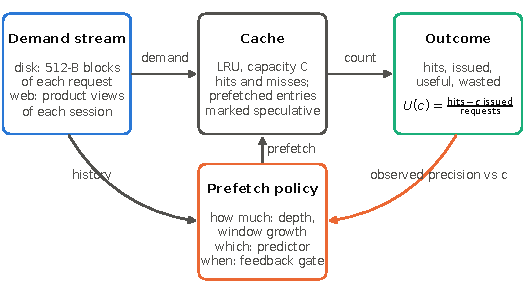
\includegraphics[width=\columnwidth]{figures/f1_schematic}
\caption{The shared abstraction. The disk study counts 512-byte blocks and the
web study counts product views; both report hits, issued, useful and wasted
prefetches, and the utility $U(c)$.}
\label{fig:f1}
\end{figure}

% >>> begin tables/t5_web_decomposition.tex
% t5_web_decomposition.tex -- GENERATED by paper/tables/make_tables.py; do not edit.
% Inputs: web/decomposition.csv
\begin{table*}[t]
\centering
\scriptsize
\setlength{\tabcolsep}{2pt}
\caption{What moves the needle (web, simulated replay): each lever's effect on the test split with a 95\% paired session-bootstrap CI, in percentage points of hit ratio (c = 0) or of utility U(c) per view.}
\label{tab:t5_web_decomposition}
\begin{tabular}{lllrlrr}
\hline
Lever & Policy vs baseline & Scorer vs baseline & Cap. & Metric (c) & $\Delta$ (pp) & Sessions \\
\hline
ranker & fixed1 vs fixed1 & trans\_s0 vs logistic & 8 & hit\_ratio (0) & $+0.07$ {\scriptsize [$+0.06$, $+0.09$]} & 364{,}364 \\
ranker & fixed1 vs fixed1 & trans\_s0 vs logistic & 8 & utility\_per\_view (0.01) & $+0.06$ {\scriptsize [$+0.05$, $+0.08$]} & 364{,}364 \\
freshness & fixed4 vs fixed4 & trans\_online vs logistic & 8 & hit\_ratio (0) & $+1.52$ {\scriptsize [$+1.49$, $+1.56$]} & 364{,}364 \\
freshness & fixed4 vs fixed4 & trans\_online vs logistic & 8 & utility\_per\_view (0.01) & $+1.48$ {\scriptsize [$+1.45$, $+1.52$]} & 364{,}364 \\
depth & fixed4 vs fixed1 & logistic & 8 & hit\_ratio (0) & $+0.80$ {\scriptsize [$+0.77$, $+0.83$]} & 364{,}364 \\
depth & fixed4 vs fixed1 & logistic & 8 & utility\_per\_view (0.01) & $-1.84$ {\scriptsize [$-1.87$, $-1.81$]} & 364{,}364 \\
controller & adaptive\_0.01 vs fixed1 & logistic & 8 & hit\_ratio (0) & $+0.26$ {\scriptsize [$+0.23$, $+0.28$]} & 364{,}364 \\
controller & adaptive\_0.01 vs fixed1 & logistic & 8 & utility\_per\_view (0.01) & $+0.36$ {\scriptsize [$+0.33$, $+0.38$]} & 364{,}364 \\
controller & adaptive\_ca\_0.01 vs fixed1 & logistic & 8 & hit\_ratio (0) & $+0.27$ {\scriptsize [$+0.25$, $+0.29$]} & 364{,}364 \\
controller & adaptive\_ca\_0.01 vs fixed1 & logistic & 8 & utility\_per\_view (0.01) & $+0.38$ {\scriptsize [$+0.36$, $+0.41$]} & 364{,}364 \\
controller & adaptive\_0.01 vs fixed1 & logistic & 32 & hit\_ratio (0) & $+0.45$ {\scriptsize [$+0.43$, $+0.48$]} & 364{,}364 \\
controller & adaptive\_0.01 vs fixed1 & logistic & 32 & utility\_per\_view (0.01) & $+0.58$ {\scriptsize [$+0.55$, $+0.61$]} & 364{,}364 \\
controller & adaptive\_ca\_0.01 vs fixed1 & logistic & 32 & hit\_ratio (0) & $+0.46$ {\scriptsize [$+0.43$, $+0.49$]} & 364{,}364 \\
controller & adaptive\_ca\_0.01 vs fixed1 & logistic & 32 & utility\_per\_view (0.01) & $+0.59$ {\scriptsize [$+0.56$, $+0.62$]} & 364{,}364 \\
feedback & feedback\_0.01\_eps0.005 vs adaptive\_0.01 & logistic & 8 & hit\_ratio (0) & $-0.11$ {\scriptsize [$-0.13$, $-0.10$]} & 364{,}364 \\
feedback & feedback\_0.01\_eps0.005 vs adaptive\_0.01 & logistic & 8 & utility\_per\_view (0.01) & $-0.01$ {\scriptsize [$-0.02$, $+0.01$]} & 364{,}364 \\
cache\_scope & fixed0 vs fixed0 & logistic & $\infty$ & hit\_ratio (0) & $+6.73$ {\scriptsize [$+6.64$, $+6.82$]} & 364{,}364 \\
sequence\_model & fixed4 vs fixed4 & seq vs trans\_online & 8 & hit\_ratio (0) & $-0.79$ {\scriptsize [$-0.83$, $-0.76$]} & 364{,}364 \\
sequence\_model & fixed4 vs fixed4 & seq vs trans\_online & 8 & utility\_per\_view (0.01) & $-0.92$ {\scriptsize [$-0.96$, $-0.88$]} & 364{,}364 \\
\hline
\end{tabular}
\end{table*}
% <<< end tables/t5_web_decomposition.tex

\textbf{Hardware and data} (Tables~\ref{tab:t1b_hardware}
and~\ref{tab:t4_web_dataset}). Table~\ref{tab:t4_web_dataset} lists every
numeric field of the web dataset profile, including the share of next views
that repeat an item already seen in the session.

% >>> begin tables/t1b_hardware.tex
% t1b_hardware.tex -- GENERATED by paper/tables/make_tables.py; do not edit.
% Inputs: disk/provenance.json, realio/device_sdb.json, realio/device_ssd.json
\begin{table*}[t]
\centering
\footnotesize
\setlength{\tabcolsep}{3pt}
\caption{Hardware of the measurement host and the calibrated devices (QD1 O\_DIRECT; $\kappa = t_{pos}/t_{xfer}$ per 512-B block).}
\label{tab:t1b_hardware}
\begin{tabular}{lllrrr}
\hline
Item & Model & Type & Rand.\ 4K p50 ($\mu$s) & Seq.\ 1M (MB/s) & $\kappa$ \\
\hline
Host & Linux-6.14.0-37-generic-x86\_64-with-glibc2.39 & 128 CPUs & -- & -- & -- \\
GPU & NVIDIA RTX PRO 6000 Blackwell Workstation Edition & shared & -- & -- & -- \\
sdb & ST10000NM017B-2T & rotational & $5629$ & $267.3$ & $2957$ \\
ssd & Micron\_5300\_MTFD & solid state & $113$ & $515.0$ & $112$ \\
\hline
\end{tabular}
\end{table*}
% <<< end tables/t1b_hardware.tex
% >>> begin tables/t4_web_dataset.tex
% t4_web_dataset.tex -- GENERATED by paper/tables/make_tables.py; do not edit.
% Inputs: web/dataset_profile.json
\begin{table}[t]
\centering
\scriptsize
\setlength{\tabcolsep}{2pt}
\caption{RetailRocket dataset profile and pair kinds, every numeric field of results/web/dataset\_profile.json as written.}
\label{tab:t4_web_dataset}
\begin{tabular}{lr}
\hline
Field & Value \\
\hline
dataset\_version & 2 \\
session\_gap\_minutes & 30 \\
raw\_rows & 2{,}756{,}101 \\
duplicate\_rows\_removed & 460 \\
event\_counts\_after\_dedup / view & 2{,}664{,}218 \\
event\_counts\_after\_dedup / addtocart & 68{,}966 \\
event\_counts\_after\_dedup / transaction & 22{,}457 \\
views & 2{,}664{,}218 \\
visitors & 1{,}407{,}580 \\
sessions & 1{,}755{,}863 \\
sessions\_with\_2plus\_views & 367{,}474 \\
sessions\_with\_3plus\_views & 158{,}980 \\
sessions\_with\_5plus\_views & 56{,}983 \\
eligible\_next\_view\_pairs & 908{,}355 \\
session\_length\_quantiles / 0.5 & $1.000$ \\
session\_length\_quantiles / 0.75 & $1.000$ \\
session\_length\_quantiles / 0.9 & $2.000$ \\
session\_length\_quantiles / 0.95 & $4.000$ \\
session\_length\_quantiles / 0.99 & $8.000$ \\
views\_by\_split / 0 & 1{,}065{,}687 \\
views\_by\_split / 1 & 532{,}844 \\
views\_by\_split / 2 & 532{,}843 \\
views\_by\_split / 3 & 532{,}844 \\
eligible\_pairs\_by\_split / 0 & 384{,}445 \\
eligible\_pairs\_by\_split / 1 & 181{,}373 \\
eligible\_pairs\_by\_split / 2 & 174{,}057 \\
eligible\_pairs\_by\_split / 3 & 168{,}480 \\
replayed\_views / validation & 532{,}843 \\
replayed\_views / test & 532{,}844 \\
pair\_kinds / validation / eligible & 174{,}057 \\
pair\_kinds / validation / kinds / novel & 111{,}554 \\
pair\_kinds / validation / kinds / self\_repeat & 42{,}986 \\
pair\_kinds / validation / kinds / earlier\_in\_session & 19{,}517 \\
pair\_kinds / validation / kinds\_share / novel & $64.09$\,\% \\
pair\_kinds / validation / kinds\_share / self\_repeat & $24.70$\,\% \\
pair\_kinds / validation / kinds\_share / earlier\_in\_session & $11.21$\,\% \\
pair\_kinds / test / eligible & 168{,}480 \\
pair\_kinds / test / kinds / novel & 106{,}765 \\
pair\_kinds / test / kinds / self\_repeat & 42{,}437 \\
pair\_kinds / test / kinds / earlier\_in\_session & 19{,}278 \\
pair\_kinds / test / kinds\_share / novel & $63.37$\,\% \\
pair\_kinds / test / kinds\_share / self\_repeat & $25.19$\,\% \\
pair\_kinds / test / kinds\_share / earlier\_in\_session & $11.44$\,\% \\
\hline
\end{tabular}
\end{table}
% <<< end tables/t4_web_dataset.tex

\textbf{Disk depth, per corpus, learned depth and $\kappa^*$}
(Fig.~\ref{fig:f2}, Tables~\ref{tab:t2b_disk_by_corpus}
and~\ref{tab:t2c_learned_depth}, Fig.~\ref{fig:f4}). The validation-chosen fixed depth is the baseline for
\texttt{learned\_depth}; the oracle column is E2's hindsight same-actions
reference, which is not a bound (it falls below the learned controller on
some traces).

\begin{figure}[t]
\centering
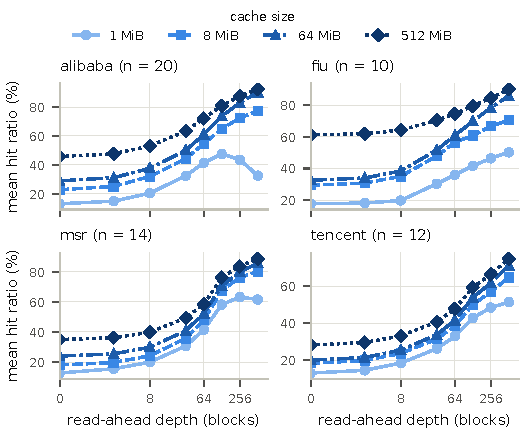
\includegraphics[width=\columnwidth]{figures/f2_hit_vs_depth}
\caption{Simulated mean block hit ratio against fixed read-ahead depth per
corpus and cache size (C2, first \diskSliceCTwo{} canonical requests per trace;
depth 0 is \texttt{none}).}
\label{fig:f2}
\end{figure}

% >>> begin tables/t2b_disk_by_corpus.tex
% t2b_disk_by_corpus.tex -- GENERATED by paper/tables/make_tables.py; do not edit.
% Inputs: disk/table_by_corpus.csv
\begin{table*}[t]
\centering
\footnotesize
\setlength{\tabcolsep}{3pt}
\caption{Disk mean block hit ratio (\%, simulated) per corpus, C1, canonical requests; n traces per corpus in the header. $^\ddagger$ demand-only Belady MIN, a reference for replacement and not a bound on prefetching.}
\label{tab:t2b_disk_by_corpus}
\begin{tabular}{lrrrrrrrr}
\hline
 & \multicolumn{4}{c}{1 MiB} & \multicolumn{4}{c}{64 MiB} \\
Policy & alibaba (20) & fiu (10) & msr (14) & tencent (12) & alibaba (20) & fiu (10) & msr (14) & tencent (12) \\
\hline
none & $14.59$ & $17.55$ & $12.95$ & $15.27$ & $30.57$ & $34.17$ & $23.88$ & $24.92$ \\
sequential & $16.38$ & $18.02$ & $16.13$ & $16.86$ & $32.69$ & $35.65$ & $25.38$ & $26.54$ \\
strided & $14.61$ & $17.40$ & $13.03$ & $15.32$ & $30.58$ & $34.26$ & $23.94$ & $24.98$ \\
stride & $14.74$ & $17.61$ & $13.87$ & $15.41$ & $30.66$ & $34.31$ & $23.97$ & $25.07$ \\
markov & $14.89$ & $17.79$ & $14.19$ & $15.71$ & $30.82$ & $34.48$ & $24.11$ & $25.39$ \\
adaptive & $15.13$ & $17.58$ & $15.11$ & $16.10$ & $31.09$ & $34.44$ & $24.41$ & $25.72$ \\
adaptive\_evidence & $15.62$ & $17.87$ & $15.48$ & $16.43$ & $31.64$ & $34.66$ & $24.72$ & $26.11$ \\
guard & $15.77$ & $17.96$ & $15.66$ & $16.35$ & $32.61$ & $35.34$ & $24.97$ & $26.34$ \\
depth\_adaptive & $18.81$ & $18.50$ & $17.75$ & $17.24$ & $37.47$ & $37.57$ & $27.32$ & $28.92$ \\
correlate & $14.82$ & $17.71$ & $15.75$ & $15.63$ & $31.35$ & $34.57$ & $24.92$ & $25.52$ \\
deep@8 & $21.85$ & $20.20$ & $20.51$ & $20.94$ & $39.03$ & $40.14$ & $29.78$ & $30.71$ \\
deep@32 & $33.69$ & $30.53$ & $30.43$ & $27.87$ & $51.17$ & $52.50$ & $40.13$ & $38.41$ \\
deep@256 & $44.23$ & $48.75$ & $63.95$ & $46.32$ & $83.67$ & $79.73$ & $80.07$ & $63.80$ \\
linux\_ra@64 & $22.50$ & $26.20$ & $17.52$ & $21.54$ & $39.57$ & $44.37$ & $26.92$ & $30.53$ \\
linux\_ra@256 & $39.58$ & $38.79$ & $41.54$ & $33.47$ & $61.34$ & $60.51$ & $52.54$ & $44.37$ \\
linux\_ra@1024 & $44.10$ & $48.58$ & $50.94$ & $38.50$ & $79.58$ & $72.94$ & $74.06$ & $54.69$ \\
belady\_min$^\ddagger$ & $23.90$ & $28.95$ & $17.66$ & $21.79$ & $40.46$ & $53.39$ & $29.98$ & $31.37$ \\
\hline
\end{tabular}
\end{table*}
% <<< end tables/t2b_disk_by_corpus.tex
% >>> begin tables/t2c_learned_depth.tex
% t2c_learned_depth.tex -- GENERATED by paper/tables/make_tables.py; do not edit.
% Inputs: gpu/disk_learned_depth.csv
\begin{table*}[t]
\centering
\footnotesize
\setlength{\tabcolsep}{3pt}
\caption{learned\_depth against the validation-chosen fixed depth (VCF) on each trace's held-out test segment (simulated block hit ratio, \%, mean over seeds). Oracle: E2's hindsight same-actions reference; it is not a bound and can fall below the learned controller.}
\label{tab:t2c_learned_depth}
\begin{tabular}{llrrrrrrr}
\hline
Trace & Corpus & Seeds & learned & VCF (depth) & deep@8 & none & Oracle & $\Delta$ vs VCF (pp) \\
\hline
\multicolumn{9}{l}{\emph{action cap 64 blocks}} \\
\hline
alibabaBlock\_13 & alibaba & 5 & $47.74$ & $49.23$ (64) & $11.74$ & $3.26$ & $39.50$ & $-1.50$ \\
alibabaBlock\_14 & alibaba & 5 & $13.47$ & $16.52$ (64) & $7.34$ & $5.72$ & $10.96$ & $-3.05$ \\
alibabaBlock\_17 & alibaba & 5 & $33.55$ & $38.04$ (64) & $25.80$ & $7.70$ & $27.62$ & $-4.49$ \\
alibabaBlock\_19 & alibaba & 5 & $60.02$ & $60.77$ (32) & $55.64$ & $45.75$ & $56.06$ & $-0.75$ \\
alibabaBlock\_23 & alibaba & 5 & $37.67$ & $44.24$ (64) & $4.84$ & $5.32$ & $28.19$ & $-6.57$ \\
alibabaBlock\_3 & alibaba & 5 & $71.21$ & $67.57$ (32) & $63.85$ & $0.94$ & $68.66$ & $+3.64$ \\
fiu\_casa-110108-112108 & fiu & 5 & $53.63$ & $54.41$ (0) & $39.67$ & $54.41$ & $44.25$ & $-0.78$ \\
fiu\_homes-110108-112108 & fiu & 5 & $28.34$ & $27.08$ (0) & $21.35$ & $27.08$ & $27.14$ & $+1.25$ \\
fiu\_madmax-110108-112108 & fiu & 5 & $47.31$ & $47.31$ (64) & $23.30$ & $18.38$ & $35.33$ & $0.00$ \\
fiu\_online.cs.fiu.edu-110108-113008 & fiu & 5 & $37.79$ & $45.87$ (64) & $19.04$ & $13.44$ & $28.39$ & $-8.07$ \\
msr\_hm\_0 & msr & 5 & $25.79$ & $29.22$ (8) & $29.22$ & $25.76$ & $32.15$ & $-3.43$ \\
msr\_prn\_0 & msr & 5 & $39.71$ & $40.38$ (64) & $37.68$ & $35.46$ & $38.14$ & $-0.67$ \\
msr\_prn\_1 & msr & 5 & $35.69$ & $40.16$ (64) & $24.49$ & $17.95$ & $29.26$ & $-4.46$ \\
msr\_proj\_0 & msr & 5 & $27.61$ & $30.72$ (64) & $7.17$ & $3.52$ & $19.46$ & $-3.11$ \\
msr\_prxy\_0 & msr & 5 & $62.33$ & $62.66$ (64) & $54.41$ & $27.27$ & $59.61$ & $-0.32$ \\
msr\_web\_2 & msr & 5 & $25.62$ & $32.62$ (64) & $3.97$ & $0.02$ & $24.39$ & $-7.01$ \\
tencentBlock\_1162 & tencent & 5 & $19.15$ & $25.14$ (64) & $3.14$ & $0.00$ & $12.79$ & $-5.99$ \\
tencentBlock\_1757 & tencent & 5 & $46.22$ & $45.00$ (4) & $45.72$ & $43.07$ & $44.88$ & $+1.22$ \\
tencentBlock\_1791 & tencent & 5 & $25.71$ & $28.87$ (64) & $18.58$ & $9.02$ & $19.72$ & $-3.16$ \\
tencentBlock\_1894 & tencent & 5 & $79.12$ & $79.35$ (64) & $76.63$ & $69.05$ & $78.67$ & $-0.23$ \\
tencentBlock\_2145 & tencent & 5 & $42.44$ & $44.91$ (64) & $20.53$ & $12.02$ & $37.56$ & $-2.48$ \\
\hline
\multicolumn{9}{l}{\emph{action cap 256 blocks}} \\
\hline
alibabaBlock\_13 & alibaba & 5 & $53.56$ & $65.91$ (128) & $11.74$ & $3.26$ & $46.70$ & $-12.35$ \\
alibabaBlock\_14 & alibaba & 5 & $23.16$ & $28.26$ (256) & $7.34$ & $5.72$ & $17.34$ & $-5.10$ \\
alibabaBlock\_17 & alibaba & 5 & $46.86$ & $48.60$ (256) & $25.80$ & $7.70$ & $36.63$ & $-1.74$ \\
alibabaBlock\_19 & alibaba & 5 & $58.18$ & $60.77$ (32) & $55.64$ & $45.75$ & $54.62$ & $-2.59$ \\
alibabaBlock\_23 & alibaba & 5 & $56.83$ & $58.89$ (256) & $4.84$ & $5.32$ & $43.88$ & $-2.06$ \\
alibabaBlock\_3 & alibaba & 5 & $91.73$ & $92.97$ (256) & $63.85$ & $0.94$ & $89.98$ & $-1.23$ \\
fiu\_casa-110108-112108 & fiu & 5 & $53.63$ & $54.41$ (0) & $39.67$ & $54.41$ & $30.36$ & $-0.78$ \\
fiu\_homes-110108-112108 & fiu & 5 & $32.15$ & $27.08$ (0) & $21.35$ & $27.08$ & $26.08$ & $+5.07$ \\
fiu\_madmax-110108-112108 & fiu & 5 & $66.74$ & $66.74$ (256) & $23.30$ & $18.38$ & $50.89$ & $0.00$ \\
fiu\_online.cs.fiu.edu-110108-113008 & fiu & 5 & $45.89$ & $50.73$ (128) & $19.04$ & $13.44$ & $37.07$ & $-4.84$ \\
msr\_hm\_0 & msr & 5 & $25.79$ & $29.22$ (8) & $29.22$ & $25.76$ & $38.88$ & $-3.43$ \\
msr\_prn\_0 & msr & 5 & $41.33$ & $40.38$ (64) & $37.68$ & $35.46$ & $38.86$ & $+0.96$ \\
msr\_prn\_1 & msr & 5 & $45.99$ & $48.69$ (256) & $24.49$ & $17.95$ & $39.32$ & $-2.70$ \\
msr\_proj\_0 & msr & 5 & $63.39$ & $64.62$ (256) & $7.17$ & $3.52$ & $46.76$ & $-1.23$ \\
msr\_prxy\_0 & msr & 5 & $59.21$ & $62.66$ (64) & $54.41$ & $27.27$ & $57.28$ & $-3.44$ \\
msr\_web\_2 & msr & 5 & $87.98$ & $93.19$ (256) & $3.97$ & $0.02$ & $85.44$ & $-5.21$ \\
tencentBlock\_1162 & tencent & 5 & $38.63$ & $50.27$ (128) & $3.14$ & $0.00$ & $26.16$ & $-11.64$ \\
tencentBlock\_1757 & tencent & 5 & $50.13$ & $45.00$ (4) & $45.72$ & $43.07$ & $49.59$ & $+5.13$ \\
tencentBlock\_1791 & tencent & 5 & $25.57$ & $29.61$ (128) & $18.58$ & $9.02$ & $20.08$ & $-4.04$ \\
tencentBlock\_1894 & tencent & 5 & $80.10$ & $79.85$ (256) & $76.63$ & $69.05$ & $79.34$ & $+0.24$ \\
tencentBlock\_2145 & tencent & 5 & $53.01$ & $54.48$ (256) & $20.53$ & $12.02$ & $47.85$ & $-1.47$ \\
\hline
\end{tabular}
\end{table*}
% <<< end tables/t2c_learned_depth.tex

\begin{figure}[t]
\centering
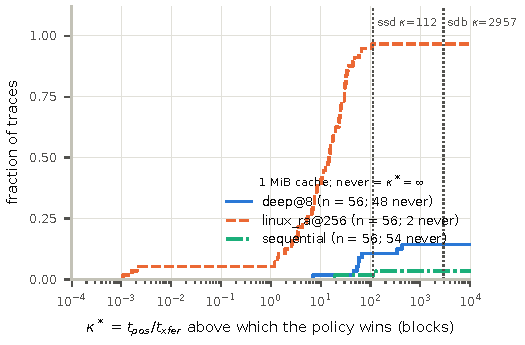
\includegraphics[width=\columnwidth]{figures/f4_kappa_cdf}
\caption{Distribution over traces of $\kappa^*$, the positioning-to-transfer
ratio above which a policy's modelled device time falls below
\texttt{none}'s (C1, 1\,MiB, simulated counts), with the measured $\kappa$ of
the two devices.}
\label{fig:f4}
\end{figure}

\textbf{Real device in detail} (Table~\ref{tab:t3_realio}): every backend and
mode on \texttt{msr\_hm\_0} on the hard disk, both think models.

% >>> begin tables/t3_realio.tex
% t3_realio.tex -- GENERATED by paper/tables/make_tables.py; do not edit.
% Inputs: realio/device_sdb.json, realio/device_ssd.json, realio/realio_summary.csv
\begin{table*}[t]
\centering
\footnotesize
\setlength{\tabcolsep}{3pt}
\caption{Real-device validation (measured). One device and trace; Backend B (odirect) replays the simulator's plan with asserted parity, Backend A (pagecache) runs through the kernel page cache. Latencies are means over repeats with 95\% CIs over repeats; k: effective prefetch multiple. Device sdb, trace msr\_hm\_0, 20{,}000 requests, 3 repeats; hit ratios in \%.}
\label{tab:t3_realio}
\begin{tabular}{llrrrrrrrrr}
\hline
Backend & Mode & Sim.\ hit & Real hit & Full-hit & Mean ($\mu$s) & p50 & p99 & Late & Dev.\ MiB & k \\
\hline
\multicolumn{11}{l}{\emph{think time closed}} \\
\hline
odirect & none & $36.10$ & $36.10$ & $43.92$ & $582$ {\scriptsize [$573$, $591$]} & $73$ & $8382$ & $0$ & $133.3$ & -- \\
odirect & sequential & $37.50$ & $37.50$ & $44.60$ & $622$ {\scriptsize [$611$, $633$]} & $85$ & $8670$ & $1033$ & $138.6$ & $1.45$ \\
odirect & adaptive\_evidence & $36.53$ & $36.53$ & $44.27$ & $612$ {\scriptsize [$584$, $639$]} & $76$ & $8623$ & $761$ & $135.3$ & $2.58$ \\
odirect & guard & $36.30$ & $36.30$ & $44.01$ & $594$ {\scriptsize [$579$, $609$]} & $73$ & $8544$ & $125$ & $134.1$ & $2.47$ \\
odirect & deep & $42.08$ & $42.08$ & $57.72$ & $619$ {\scriptsize [$597$, $642$]} & $20$ & $8773$ & $1108$ & $153.7$ & $0.63$ \\
odirect & deep@64 & $55.92$ & $55.92$ & $71.57$ & $646$ {\scriptsize [$641$, $651$]} & $9$ & $9236$ & $903$ & $257.6$ & $0.33$ \\
odirect & linux\_ra & $45.23$ & $45.23$ & $53.14$ & $590$ {\scriptsize [$583$, $597$]} & $42$ & $8474$ & $414$ & $145.8$ & $0.65$ \\
pagecache & none & $36.10$ & $35.85$ & $44.75$ & $556$ {\scriptsize [$548$, $564$]} & $67$ & $8279$ & $0$ & $136.5$ & -- \\
pagecache & sequential & $37.50$ & $38.95$ & $54.18$ & $580$ {\scriptsize [$571$, $589$]} & $12$ & $8620$ & $152$ & $157.0$ & $1.46$ \\
pagecache & adaptive\_evidence & $36.53$ & $35.78$ & $48.74$ & $573$ {\scriptsize [$572$, $574$]} & $51$ & $8557$ & $107$ & $151.6$ & $1.22$ \\
pagecache & guard & $36.30$ & $36.49$ & $46.00$ & $560$ {\scriptsize [$556$, $564$]} & $66$ & $8332$ & $16$ & $139.0$ & $1.52$ \\
pagecache & deep & $42.08$ & $42.17$ & $55.36$ & $580$ {\scriptsize [$570$, $589$]} & $8$ & $8645$ & $148$ & $152.9$ & $0.58$ \\
pagecache & deep@64 & $55.92$ & $51.71$ & $67.29$ & $611$ {\scriptsize [$599$, $622$]} & $4$ & $9118$ & $201$ & $260.8$ & $0.31$ \\
pagecache & linux\_ra & $45.23$ & $36.68$ & $47.47$ & $559$ {\scriptsize [$540$, $578$]} & $48$ & $8439$ & $134$ & $162.4$ & $0.06$ \\
pagecache & kernel\_ra & -- & $50.61$ & $55.62$ & $558$ {\scriptsize [$533$, $583$]} & $8$ & $8424$ & $135$ & $174.6$ & -- \\
pagecache & kernel\_seq & -- & $51.31$ & $55.78$ & $566$ {\scriptsize [$547$, $585$]} & $7$ & $8397$ & $144$ & $204.9$ & -- \\
pagecache & online-guard & $36.30$ & $25.47$ & $38.50$ & $570$ {\scriptsize [$550$, $590$]} & $67$ & $8327$ & $10$ & $162.0$ & $-16.64$ \\
\hline
\multicolumn{11}{l}{\emph{think time spread:1:5000}} \\
\hline
odirect & none & $36.10$ & $36.10$ & $43.92$ & $844$ {\scriptsize [$794$, $895$]} & $95$ & $13853$ & $0$ & $133.3$ & -- \\
odirect & sequential & $37.50$ & $37.50$ & $44.60$ & $826$ {\scriptsize [$817$, $835$]} & $86$ & $11912$ & $18$ & $138.6$ & $0.02$ \\
odirect & adaptive\_evidence & $36.53$ & $36.53$ & $44.27$ & $835$ {\scriptsize [$801$, $870$]} & $94$ & $11755$ & $20$ & $135.3$ & $-0.11$ \\
odirect & guard & $36.30$ & $36.30$ & $44.01$ & $822$ {\scriptsize [$783$, $861$]} & $95$ & $11366$ & $1$ & $134.1$ & $-2.56$ \\
odirect & deep & $42.08$ & $42.08$ & $57.72$ & $846$ {\scriptsize [$790$, $902$]} & $39$ & $14601$ & $29$ & $153.7$ & $0.39$ \\
odirect & deep@64 & $55.92$ & $55.92$ & $71.57$ & $896$ {\scriptsize [$881$, $910$]} & $30$ & $17101$ & $20$ & $257.6$ & $0.30$ \\
odirect & linux\_ra & $45.23$ & $45.23$ & $53.14$ & $889$ {\scriptsize [$885$, $892$]} & $59$ & $16071$ & $21$ & $145.8$ & $0.83$ \\
pagecache & none & $36.10$ & $35.76$ & $44.77$ & $754$ {\scriptsize [$632$, $877$]} & $73$ & $12445$ & $0$ & $136.7$ & -- \\
pagecache & sequential & $37.50$ & $41.98$ & $57.38$ & $711$ {\scriptsize [$697$, $725$]} & $16$ & $13253$ & $3$ & $153.0$ & $0.67$ \\
pagecache & adaptive\_evidence & $36.53$ & $39.72$ & $52.86$ & $758$ {\scriptsize [$683$, $832$]} & $20$ & $13775$ & $1$ & $145.5$ & $3.15$ \\
pagecache & guard & $36.30$ & $36.18$ & $45.80$ & $758$ {\scriptsize [$726$, $790$]} & $70$ & $13778$ & $0$ & $139.9$ & $1.57$ \\
pagecache & deep & $42.08$ & $42.19$ & $57.95$ & $665$ {\scriptsize [$443$, $888$]} & $18$ & $12649$ & $5$ & $155.4$ & $-0.09$ \\
pagecache & deep@64 & $55.92$ & $56.12$ & $71.69$ & $756$ {\scriptsize [$591$, $921$]} & $11$ & $15641$ & $5$ & $258.0$ & $0.29$ \\
pagecache & linux\_ra & $45.23$ & $45.25$ & $53.65$ & $841$ {\scriptsize [$721$, $960$]} & $19$ & $16007$ & $4$ & $147.9$ & $1.13$ \\
pagecache & kernel\_ra & -- & $48.18$ & $54.78$ & $841$ {\scriptsize [$825$, $857$]} & $25$ & $16392$ & $6$ & $182.7$ & -- \\
pagecache & kernel\_seq & -- & $51.29$ & $55.78$ & $780$ {\scriptsize [$734$, $826$]} & $19$ & $15770$ & $4$ & $204.4$ & -- \\
pagecache & online-guard & $36.30$ & $25.99$ & $39.06$ & $769$ {\scriptsize [$741$, $797$]} & $87$ & $12529$ & $0$ & $161.3$ & $-15.47$ \\
\hline
\end{tabular}
\end{table*}
% <<< end tables/t3_realio.tex

\textbf{Web comparisons and freshness} (Table~\ref{tab:t6_web_comparisons},
Fig.~\ref{fig:f6}).

% >>> begin tables/t6_web_comparisons.tex
% t6_web_comparisons.tex -- GENERATED by paper/tables/make_tables.py; do not edit.
% Inputs: web/comparisons.csv
\begin{table*}[t]
\centering
\scriptsize
\setlength{\tabcolsep}{2pt}
\caption{Validated web controllers against the strongest fair baselines (test split, simulated, per-capacity selection on validation, assumed c = 0.01): the best fixed depth at the same capacity, no prefetch (fixed0) and transition top-1. $\Delta$ U(c) per view in percentage points with 95\% paired session-bootstrap CIs.}
\label{tab:t6_web_comparisons}
\begin{tabular}{rrllrrrl}
\hline
Cap. & c & Selected & Best fixed & vs best fixed & vs fixed0 & vs trans.\ top-1 & Label \\
\hline
\multicolumn{8}{l}{\emph{per\_capacity selection, scorer logistic}} \\
\hline
2 & 0.01 & adaptive\_0.1 & fixed0 & $+0.04$ {\scriptsize [$+0.03$, $+0.05$]} & $+0.04$ {\scriptsize [$+0.03$, $+0.05$]} & $+2.46$ {\scriptsize [$+2.40$, $+2.52$]} & adaptive wins \\
2 & 0.01 & adaptive\_ca\_0.1 & fixed0 & $+0.04$ {\scriptsize [$+0.03$, $+0.05$]} & $+0.04$ {\scriptsize [$+0.03$, $+0.05$]} & $+2.46$ {\scriptsize [$+2.40$, $+2.52$]} & adaptive\_ca wins \\
2 & 0.01 & gate\_0.1 & fixed0 & $-0.33$ {\scriptsize [$-0.35$, $-0.31$]} & $-0.33$ {\scriptsize [$-0.35$, $-0.31$]} & $+2.09$ {\scriptsize [$+2.03$, $+2.15$]} & gate loses to no prefetch \\
2 & 0.01 & feedback\_0.05\_eps0.0005 & fixed0 & $+0.01$ {\scriptsize [$0.00$, $+0.01$]} & $+0.01$ {\scriptsize [$0.00$, $+0.01$]} & $+2.43$ {\scriptsize [$+2.37$, $+2.49$]} & feedback within noise \\
4 & 0.01 & adaptive\_0.02 & fixed0 & $+0.20$ {\scriptsize [$+0.17$, $+0.22$]} & $+0.20$ {\scriptsize [$+0.17$, $+0.22$]} & $+0.34$ {\scriptsize [$+0.31$, $+0.36$]} & adaptive wins \\
4 & 0.01 & adaptive\_ca\_0.02 & fixed0 & $+0.21$ {\scriptsize [$+0.18$, $+0.23$]} & $+0.21$ {\scriptsize [$+0.18$, $+0.23$]} & $+0.35$ {\scriptsize [$+0.32$, $+0.37$]} & adaptive\_ca wins \\
4 & 0.01 & gate\_0.02 & fixed0 & $+0.12$ {\scriptsize [$+0.10$, $+0.14$]} & $+0.12$ {\scriptsize [$+0.10$, $+0.14$]} & $+0.26$ {\scriptsize [$+0.23$, $+0.28$]} & gate wins \\
4 & 0.01 & feedback\_0.02\_eps0.0005 & fixed0 & $+0.06$ {\scriptsize [$+0.05$, $+0.07$]} & $+0.06$ {\scriptsize [$+0.05$, $+0.07$]} & $+0.20$ {\scriptsize [$+0.17$, $+0.23$]} & feedback wins \\
8 & 0.01 & adaptive\_0.01 & fixed1 & $+0.36$ {\scriptsize [$+0.33$, $+0.38$]} & $+0.44$ {\scriptsize [$+0.41$, $+0.48$]} & $+0.30$ {\scriptsize [$+0.27$, $+0.32$]} & adaptive wins \\
8 & 0.01 & adaptive\_ca\_0.01 & fixed1 & $+0.38$ {\scriptsize [$+0.36$, $+0.41$]} & $+0.47$ {\scriptsize [$+0.44$, $+0.50$]} & $+0.32$ {\scriptsize [$+0.30$, $+0.35$]} & adaptive\_ca wins \\
8 & 0.01 & gate\_0.01 & fixed1 & $+0.31$ {\scriptsize [$+0.29$, $+0.33$]} & $+0.40$ {\scriptsize [$+0.37$, $+0.43$]} & $+0.25$ {\scriptsize [$+0.23$, $+0.27$]} & gate wins \\
8 & 0.01 & feedback\_0.01\_eps0.005 & fixed1 & $+0.35$ {\scriptsize [$+0.32$, $+0.37$]} & $+0.44$ {\scriptsize [$+0.40$, $+0.47$]} & $+0.29$ {\scriptsize [$+0.26$, $+0.31$]} & feedback wins \\
16 & 0.01 & adaptive\_0.01 & fixed1 & $+0.53$ {\scriptsize [$+0.50$, $+0.55$]} & $+0.69$ {\scriptsize [$+0.65$, $+0.73$]} & $+0.46$ {\scriptsize [$+0.43$, $+0.48$]} & adaptive wins \\
16 & 0.01 & adaptive\_ca\_0.01 & fixed1 & $+0.53$ {\scriptsize [$+0.51$, $+0.56$]} & $+0.70$ {\scriptsize [$+0.66$, $+0.73$]} & $+0.47$ {\scriptsize [$+0.44$, $+0.49$]} & adaptive\_ca wins \\
16 & 0.01 & gate\_0.01 & fixed1 & $+0.38$ {\scriptsize [$+0.36$, $+0.40$]} & $+0.54$ {\scriptsize [$+0.51$, $+0.57$]} & $+0.31$ {\scriptsize [$+0.29$, $+0.33$]} & gate wins \\
16 & 0.01 & feedback\_0.01\_eps0.0005 & fixed1 & $+0.50$ {\scriptsize [$+0.48$, $+0.52$]} & $+0.66$ {\scriptsize [$+0.63$, $+0.70$]} & $+0.43$ {\scriptsize [$+0.41$, $+0.45$]} & feedback wins \\
32 & 0.01 & adaptive\_0.01 & fixed1 & $+0.58$ {\scriptsize [$+0.55$, $+0.61$]} & $+0.77$ {\scriptsize [$+0.73$, $+0.81$]} & $+0.51$ {\scriptsize [$+0.49$, $+0.54$]} & adaptive wins \\
32 & 0.01 & adaptive\_ca\_0.01 & fixed1 & $+0.59$ {\scriptsize [$+0.56$, $+0.62$]} & $+0.78$ {\scriptsize [$+0.74$, $+0.81$]} & $+0.52$ {\scriptsize [$+0.50$, $+0.55$]} & adaptive\_ca wins \\
32 & 0.01 & gate\_0.01 & fixed1 & $+0.41$ {\scriptsize [$+0.38$, $+0.43$]} & $+0.59$ {\scriptsize [$+0.56$, $+0.63$]} & $+0.34$ {\scriptsize [$+0.32$, $+0.36$]} & gate wins \\
32 & 0.01 & feedback\_0.01\_eps0.0005 & fixed1 & $+0.54$ {\scriptsize [$+0.51$, $+0.56$]} & $+0.72$ {\scriptsize [$+0.69$, $+0.76$]} & $+0.47$ {\scriptsize [$+0.44$, $+0.49$]} & feedback wins \\
\hline
\multicolumn{8}{l}{\emph{per\_capacity selection, scorer trans\_online}} \\
\hline
2 & 0.01 & adaptive\_0.2 & fixed0 & $-0.25$ {\scriptsize [$-0.28$, $-0.21$]} & $-0.25$ {\scriptsize [$-0.28$, $-0.21$]} & $+2.18$ {\scriptsize [$+2.13$, $+2.23$]} & adaptive loses to no prefetch \\
2 & 0.01 & adaptive\_ca\_0.2 & fixed0 & $-0.24$ {\scriptsize [$-0.28$, $-0.21$]} & $-0.24$ {\scriptsize [$-0.28$, $-0.21$]} & $+2.19$ {\scriptsize [$+2.13$, $+2.24$]} & adaptive\_ca loses to no prefetch \\
2 & 0.01 & gate\_0.1 & fixed0 & $-2.19$ {\scriptsize [$-2.24$, $-2.14$]} & $-2.19$ {\scriptsize [$-2.24$, $-2.14$]} & $+0.23$ {\scriptsize [$+0.19$, $+0.29$]} & gate loses to no prefetch \\
2 & 0.01 & feedback\_0.02\_eps0.0005 & fixed0 & $-0.17$ {\scriptsize [$-0.19$, $-0.14$]} & $-0.17$ {\scriptsize [$-0.19$, $-0.14$]} & $+2.25$ {\scriptsize [$+2.20$, $+2.32$]} & feedback loses to no prefetch \\
4 & 0.01 & adaptive\_0.2 & fixed1 & $-0.13$ {\scriptsize [$-0.16$, $-0.10$]} & $+0.50$ {\scriptsize [$+0.48$, $+0.53$]} & $+0.64$ {\scriptsize [$+0.61$, $+0.68$]} & adaptive loses \\
4 & 0.01 & adaptive\_ca\_0.2 & fixed1 & $-0.12$ {\scriptsize [$-0.16$, $-0.09$]} & $+0.51$ {\scriptsize [$+0.48$, $+0.54$]} & $+0.65$ {\scriptsize [$+0.62$, $+0.68$]} & adaptive\_ca loses \\
4 & 0.01 & gate\_0.1 & fixed1 & $-0.01$ {\scriptsize [$-0.04$, $+0.03$]} & $+0.62$ {\scriptsize [$+0.58$, $+0.66$]} & $+0.76$ {\scriptsize [$+0.73$, $+0.80$]} & gate within noise \\
4 & 0.01 & feedback\_0.02\_eps0.002 & fixed1 & $+0.07$ {\scriptsize [$+0.05$, $+0.09$]} & $+0.70$ {\scriptsize [$+0.66$, $+0.73$]} & $+0.84$ {\scriptsize [$+0.81$, $+0.87$]} & feedback wins \\
8 & 0.01 & adaptive\_0.1 & fixed1 & $+0.20$ {\scriptsize [$+0.17$, $+0.23$]} & $+1.13$ {\scriptsize [$+1.08$, $+1.17$]} & $+0.98$ {\scriptsize [$+0.94$, $+1.02$]} & adaptive wins \\
8 & 0.01 & adaptive\_ca\_0.1 & fixed1 & $+0.22$ {\scriptsize [$+0.19$, $+0.25$]} & $+1.14$ {\scriptsize [$+1.10$, $+1.19$]} & $+0.99$ {\scriptsize [$+0.96$, $+1.03$]} & adaptive\_ca wins \\
8 & 0.01 & gate\_0.05 & fixed1 & $+0.30$ {\scriptsize [$+0.27$, $+0.33$]} & $+1.22$ {\scriptsize [$+1.18$, $+1.26$]} & $+1.07$ {\scriptsize [$+1.03$, $+1.11$]} & gate wins \\
8 & 0.01 & feedback\_0.01\_eps0.005 & fixed1 & $+0.25$ {\scriptsize [$+0.22$, $+0.29$]} & $+1.18$ {\scriptsize [$+1.13$, $+1.22$]} & $+1.03$ {\scriptsize [$+0.99$, $+1.07$]} & feedback wins \\
16 & 0.01 & adaptive\_0.05 & fixed2 & $+0.27$ {\scriptsize [$+0.24$, $+0.30$]} & $+1.38$ {\scriptsize [$+1.32$, $+1.44$]} & $+1.15$ {\scriptsize [$+1.10$, $+1.21$]} & adaptive wins \\
16 & 0.01 & adaptive\_ca\_0.05 & fixed2 & $+0.26$ {\scriptsize [$+0.23$, $+0.29$]} & $+1.37$ {\scriptsize [$+1.31$, $+1.43$]} & $+1.14$ {\scriptsize [$+1.09$, $+1.19$]} & adaptive\_ca wins \\
16 & 0.01 & gate\_0.05 & fixed2 & $+0.35$ {\scriptsize [$+0.34$, $+0.35$]} & $+1.46$ {\scriptsize [$+1.42$, $+1.51$]} & $+1.23$ {\scriptsize [$+1.19$, $+1.28$]} & gate wins \\
16 & 0.01 & feedback\_0.01\_eps0.0005 & fixed2 & $+0.48$ {\scriptsize [$+0.46$, $+0.50$]} & $+1.60$ {\scriptsize [$+1.55$, $+1.65$]} & $+1.37$ {\scriptsize [$+1.32$, $+1.41$]} & feedback wins \\
32 & 0.01 & adaptive\_0.05 & fixed2 & $+0.45$ {\scriptsize [$+0.42$, $+0.49$]} & $+1.67$ {\scriptsize [$+1.61$, $+1.73$]} & $+1.41$ {\scriptsize [$+1.36$, $+1.47$]} & adaptive wins \\
32 & 0.01 & adaptive\_ca\_0.05 & fixed2 & $+0.45$ {\scriptsize [$+0.41$, $+0.48$]} & $+1.66$ {\scriptsize [$+1.60$, $+1.72$]} & $+1.40$ {\scriptsize [$+1.35$, $+1.46$]} & adaptive\_ca wins \\
32 & 0.01 & gate\_0.02 & fixed2 & $+0.33$ {\scriptsize [$+0.33$, $+0.34$]} & $+1.55$ {\scriptsize [$+1.50$, $+1.60$]} & $+1.29$ {\scriptsize [$+1.25$, $+1.33$]} & gate wins \\
32 & 0.01 & feedback\_0.01\_eps0.005 & fixed2 & $+0.57$ {\scriptsize [$+0.54$, $+0.59$]} & $+1.78$ {\scriptsize [$+1.72$, $+1.84$]} & $+1.52$ {\scriptsize [$+1.48$, $+1.57$]} & feedback wins \\
\hline
\end{tabular}
\\[2pt]{\scriptsize Bootstrap: 500 session resamples.}
\end{table*}
% <<< end tables/t6_web_comparisons.tex

\begin{figure}[t]
\centering
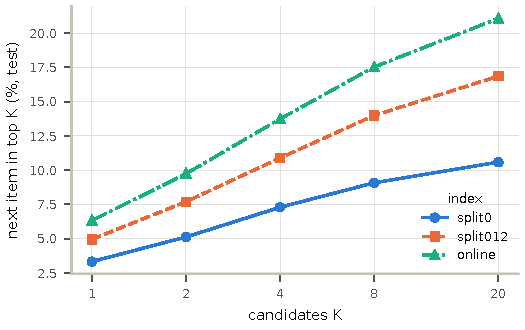
\includegraphics[width=\columnwidth]{figures/f6_freshness}
\caption{Share of eligible test views whose next item is among the top $K$
candidates of the index-split counts, the counts of splits 0--2, and the
online counts (simulated, descriptive).}
\label{fig:f6}
\end{figure}

\textbf{Live ablations and the bytes trade-off} (Table~\ref{tab:t7b_live_ablation},
Fig.~\ref{fig:f7}).

% >>> begin tables/t7b_live_ablation.tex
% t7b_live_ablation.tex -- GENERATED by paper/tables/make_tables.py; do not edit.
% Inputs: live/live_metrics.csv
\begin{table*}[t]
\centering
\footnotesize
\setlength{\tabcolsep}{3pt}
\caption{Live HTTP ablations (measured, loopback, ASSUMED network): FIFO link, hint and sensitivity passes; milliseconds saved per view against the baseline.}
\label{tab:t7b_live_ablation}
\begin{tabular}{lllrrr}
\hline
Experiment & Store / link & Policy & Passes & Saved (ms) & Ideal \\
\hline
fifo & ssd / fifo & fixed0 & 1 & $0.00$ {\scriptsize [$0.00$, $0.00$]} & $0.00$ \\
fifo & ssd / fifo & fixed4 & 1 & $4.79$ {\scriptsize [$3.76$, $5.99$]} & $5.09$ \\
fifo & ssd / fifo & fixed8 & 1 & $1.22$ {\scriptsize [$-0.14$, $2.44$]} & $3.32$ \\
hint & hdd / priority & fixed0 & 1 & $0.00$ {\scriptsize [$0.00$, $0.00$]} & $0.00$ \\
hint & hdd / priority & hint:fixed4 & 1 & $1.48$ {\scriptsize [$1.24$, $1.74$]} & $0.00$ \\
hint & hdd / priority & hint:fixed8 & 1 & $1.75$ {\scriptsize [$1.49$, $2.01$]} & $0.00$ \\
\hline
\end{tabular}
\end{table*}
% <<< end tables/t7b_live_ablation.tex

\begin{figure}[t]
\centering
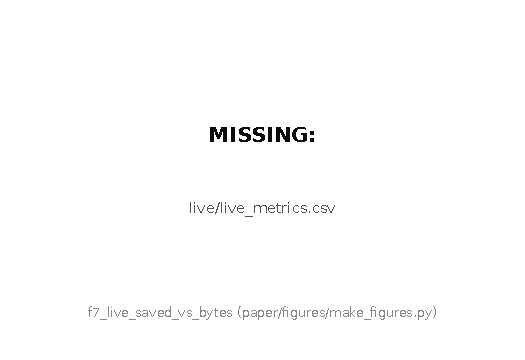
\includegraphics[width=\columnwidth]{figures/f7_live_saved_vs_bytes}
\caption{Measured wait saved per view against wasted KiB per view, per store
and policy (loopback, emulated network, assumed sizes; citable passes only).}
\label{fig:f7}
\end{figure}

\textbf{Cross-domain summary} (Table~\ref{tab:t8_cross_domain}).

% >>> begin tables/t8_cross_domain.tex
% t8_cross_domain.tex -- GENERATED by paper/tables/make_tables.py; do not edit.
% Inputs: disk/sweep.jsonl, disk/table_main.csv, live/live_metrics.csv, web/comparisons.csv, web/decomposition.csv, web/policy_metrics.csv
\begin{table*}[t]
\centering
\scriptsize
\setlength{\tabcolsep}{2pt}
\caption{Cross-domain summary. Disk and web rows are simulated, live rows measured on loopback with an ASSUMED network. Gain is against no prefetching with a 95\% CI; c*: the cost per prefetch at which the policy ties no prefetching.}
\label{tab:t8_cross_domain}
\begin{tabular}{lllrrrr}
\hline
Domain / setting & Policy & Gain unit & Gain over none & Waste; I/Os & c* & Feedback gate \\
\hline
Disk, 1 MiB & deep@256 & hit ratio, pp & $+35.56$ {\scriptsize [$+29.03$, $+41.86$]} & $80.72$\,\% unused, $1.309\times$ I/Os & $0.076$ & $+1.40$ {\scriptsize [$+0.70$, $+2.46$]} \\
Disk, 64 MiB & deep@256 & hit ratio, pp & $+49.48$ {\scriptsize [$+43.50$, $+55.62$]} & $47.54$\,\% unused, $1.147\times$ I/Os & $0.418$ & $+1.52$ {\scriptsize [$+1.17$, $+1.89$]} \\
Web, cap.\ 2, c = 0.01 & adaptive\_0.1 & U per view, pp & $+0.04$ {\scriptsize [$+0.03$, $+0.05$]} & $0.00$ /view & $0.0874$ & -- \\
Web, cap.\ 4, c = 0.01 & adaptive\_0.02 & U per view, pp & $+0.20$ {\scriptsize [$+0.17$, $+0.22$]} & $0.21$ /view & $0.0192$ & -- \\
Web, cap.\ 8, c = 0.01 & adaptive\_0.01 & U per view, pp & $+0.44$ {\scriptsize [$+0.41$, $+0.48$]} & $0.72$ /view & $0.0160$ & $-0.01$ {\scriptsize [$-0.02$, $+0.01$]} \\
Web, cap.\ 16, c = 0.01 & adaptive\_0.01 & U per view, pp & $+0.69$ {\scriptsize [$+0.65$, $+0.73$]} & $0.69$ /view & $0.0198$ & -- \\
Web, cap.\ 32, c = 0.01 & adaptive\_0.01 & U per view, pp & $+0.77$ {\scriptsize [$+0.73$, $+0.81$]} & $0.68$ /view & $0.0211$ & -- \\
Live HTTP, hdd store & adaptive\_0.1@trans\_online & ms per view & $8.27$ {\scriptsize [$7.09$, $9.73$]} & $95.4$ KiB & -- & $6.99$ {\scriptsize [$5.95$, $8.19$]} \\
Live HTTP, ssd store & adaptive\_0.1@trans\_online & ms per view & $6.36$ {\scriptsize [$5.34$, $7.51$]} & $95.4$ KiB & -- & $4.58$ {\scriptsize [$3.72$, $5.67$]} \\
\hline
\end{tabular}
\\[2pt]{\scriptsize Disk: C1 canonical, the highest mean hit ratio (not a winner: its waste and device I/Os are beside it); gate column: guard's hit-ratio gain over none. Web: the validation-selected controller at the smallest positive cost; gate column: the validated feedback gate minus the adaptive controller in U at that cost (W6). Live: the citable policy with the largest mean saving; gate column: the feedback gate's own saving per view.}
\end{table*}
% <<< end tables/t8_cross_domain.tex

\section{The Classifier Study in Detail}\label{app:classifiers}

\textbf{The families.} Gaussian naive
Bayes~\cite{domingos1997optimality,zhang2004optimality}, LDA~\cite{fisher1936use}
with shrinkage~\cite{ledoit2004well}, QDA~\cite{hastie2009elements}, logistic
regression~\cite{cox1958regression}, $k$-nearest
neighbours~\cite{cover1967nearest}, linear and RBF
SVMs~\cite{cortes1995support} with Platt
probabilities~\cite{platt1999probabilistic}, CART~\cite{breiman1984cart},
random forests~\cite{breiman2001random}, extremely randomised
trees~\cite{geurts2006extremely}, histogram gradient
boosting~\cite{friedman2001greedy,ke2017lightgbm}, an
MLP~\cite{rumelhart1986learning} trained with Adam~\cite{kingma2015adam} and
logistic SGD trained online~\cite{bottou2010large}, all in
scikit-learn~\cite{pedregosa2011sklearn}; a streaming Hoeffding
tree~\cite{domingos2000mining} was not run. Selection used
\clfSynFolds{} folds over the training seeds.

\textbf{Synthetic windows} (Table~\ref{tab:t10_classifier_zoo}). Each cell is
the mean test accuracy over \clfSynSeedPairs{} pairs of independent training
and test seeds, after selection on the training seeds alone. The settings are
those of the earlier synthetic evaluation, on the twelve contextual features
the router uses; the transfer columns are the block-size shift. Under it,
\decTallyClfZeroTransferOneToThirtyTwoWorse{} of
\decTallyClfZeroTransferOneToThirtyTwo{} families, the scale-sensitive ones
among them, are worse than GNB at the 32-block size. On the heaviest phase blend GNB
scores \clfSynAccTransitionHeavyGnbOnline{} and a random forest
\clfSynAccTransitionHeavyRf{} (\clfSynDeltaTransitionHeavyRfCI), a margin that
is optimistic because each window's context comes from earlier windows of the
same class.

% >>> begin tables/t10_classifier_zoo.tex
% t10_classifier_zoo.tex -- GENERATED by paper/tables/make_tables.py; do not edit.
% Inputs: classifier/router_comparisons.csv, classifier/synthetic_eval.csv
\begin{table*}[t]
\centering
\scriptsize
\setlength{\tabcolsep}{2pt}
\caption{Classifier zoo on synthetic windows (track CLF, Part 1; \emph{synthetic} test accuracy, mean over independent test seeds, never an accuracy on real traces). Every tuned family was selected by random search on training seeds only; \texttt{gnb\_online} and \texttt{qda\_online} are the shipped models, untuned. $^{+}$/$^{-}$: better/worse than \texttt{gnb\_online} by the paired bootstrap over seed pairs; no mark: no difference detected. Transfer: trained on single-block requests, tested at the request size shown (block-size covariate shift). The context features come from earlier windows of the same class, which favours the phase-blend settings.}
\label{tab:t10_classifier_zoo}
\begin{tabular}{lrrrrrrrrrrr}
\hline
Family & base. & noisy & ovl. & ovl.\,2 & real. & trans. & trans.\ heavy & 1$\to$1 & 1$\to$8 & 1$\to$32 & 1$\to$128 \\
\hline
gnb\_online & $0.996$ & $0.999$ & $0.996$ & $0.998$ & $1.000$ & $0.666$ & $0.510$ & $1.000$ & $0.972$ & $1.000$ & $1.000$ \\
qda\_online & $0.999^{+}$ & $0.996^{-}$ & $1.000^{+}$ & $1.000$ & $1.000$ & $0.660$ & $0.828^{+}$ & $1.000$ & $0.868^{-}$ & $0.854^{-}$ & $0.854^{-}$ \\
gnb & $0.999^{+}$ & $0.999$ & $1.000^{+}$ & $1.000$ & $1.000$ & $0.669$ & $0.698^{+}$ & $0.999$ & $0.971$ & $1.000$ & $1.000$ \\
lda & $0.999^{+}$ & $0.999$ & $1.000^{+}$ & $1.000$ & $1.000$ & $0.647^{-}$ & $0.291^{-}$ & $1.000$ & $0.826^{-}$ & $0.750^{-}$ & $0.750^{-}$ \\
qda & $0.910^{-}$ & $0.984^{-}$ & $0.990^{-}$ & $0.979^{-}$ & $0.995^{-}$ & $0.630^{-}$ & $0.418^{-}$ & $0.981^{-}$ & $0.969$ & $1.000$ & $1.000$ \\
logreg & $0.999^{+}$ & $0.999$ & $1.000^{+}$ & $1.000$ & $1.000$ & $0.652$ & $0.288^{-}$ & $0.999$ & $0.807^{-}$ & $0.750^{-}$ & $0.750^{-}$ \\
knn & $0.990^{-}$ & $0.992^{-}$ & $0.998$ & $0.998$ & $0.997^{-}$ & $0.647$ & $0.886^{+}$ & $0.992^{-}$ & $0.757^{-}$ & $0.750^{-}$ & $0.750^{-}$ \\
svm\_linear & $0.999^{+}$ & $0.999$ & $1.000^{+}$ & $1.000$ & $1.000$ & $0.657$ & $0.288^{-}$ & $1.000$ & $0.755^{-}$ & $0.750^{-}$ & $0.750^{-}$ \\
svm\_rbf & $0.999^{+}$ & $0.999$ & $1.000^{+}$ & $1.000$ & $1.000$ & $0.661$ & $0.929^{+}$ & $1.000$ & $0.750^{-}$ & $0.750^{-}$ & $0.750^{-}$ \\
cart & $0.997$ & $0.999$ & $0.999$ & $0.999$ & $0.999$ & $0.635^{-}$ & $0.968^{+}$ & $1.000$ & $0.972$ & $1.000$ & $1.000$ \\
rf & $0.999^{+}$ & $0.999$ & $0.999$ & $1.000$ & $1.000$ & $0.651$ & $0.968^{+}$ & $1.000$ & $0.972$ & $1.000$ & $1.000$ \\
extra\_trees & $1.000^{+}$ & $0.998$ & $0.999^{+}$ & $1.000$ & $1.000$ & $0.664$ & $0.964^{+}$ & $0.998$ & $0.963^{-}$ & $1.000$ & $1.000$ \\
hgb & $0.996$ & $0.999$ & $1.000^{+}$ & $1.000$ & $0.998$ & $0.669$ & $0.965^{+}$ & $1.000$ & $0.970$ & $1.000$ & $1.000$ \\
mlp & $0.998$ & $0.999$ & $0.998$ & $1.000$ & $0.999$ & $0.664$ & $0.946^{+}$ & $0.998$ & $0.957$ & $0.903^{-}$ & $0.903^{-}$ \\
sgd\_online & $0.941^{-}$ & $0.998$ & $0.998$ & $0.999$ & $0.999$ & $0.640^{-}$ & $0.278^{-}$ & $0.999$ & $0.977^{+}$ & $1.000$ & $1.000$ \\
\hline
\end{tabular}
\\[2pt]{\scriptsize 12 seed pairs per cell; 10{,}000 bootstrap resamples.}
\end{table*}
% <<< end tables/t10_classifier_zoo.tex

\textbf{The routed classifiers} (Table~\ref{tab:t11_classifier_router}). The
shipped GNB through the precomputed-label replay reproduces E1's
\texttt{adaptive} rows on every counter, and the reference rows are E1's own.
At 64\,MiB, \decTallyClfTwoSixtyFourMiBBetter{} alternatives are better than the
shipped GNB (\decClfClaimTunedBetterSixtyFourMiBVerdict) and every routed
classifier is worse than \texttt{sequential}; all of them increase device I/Os
and move more blocks than \texttt{none}.

% >>> begin tables/t11_classifier_router.tex
% t11_classifier_router.tex -- GENERATED by paper/tables/make_tables.py; do not edit.
% Inputs: classifier/router_comparisons.csv, classifier/router_summary.csv
\begin{table*}[t]
\centering
\scriptsize
\setlength{\tabcolsep}{2pt}
\caption{Routed \texttt{adaptive} with each classifier on real traces (track CLF, Part 2; simulated LRU cache, C3 slice 2, writes replay as reads). Hit ratio is the mean over traces; $\Delta$ in pp with the paired-bootstrap interval over traces, $^{+}$/$^{-}$ when the paired and the corpus-cluster interval agree on better/worse; device-I/O and blocks-moved ratios are means over traces of the policy's count over \texttt{none}'s; agreement is the share of windows given the shipped GNB's class.}
\label{tab:t11_classifier_router}
\begin{tabular}{lrrrrrrr}
\hline
Policy & Hit (\%) & $\Delta$ vs sequential & $\Delta$ vs gnb\_online & Dev.\ I/O & Blocks & Prec.\ (\%) & Agree \\
\hline
\multicolumn{8}{l}{\emph{1 MiB cache (2{,}048 blocks), n = 19 traces}} \\
\hline
none & $21.75$ & -- & -- & $1.000\times$ & $1.000\times$ & -- & -- \\
sequential & $24.26$ & -- & -- & $1.072\times$ & $1.070\times$ & $46.9$ & -- \\
deep@8 & $28.89$ & $+4.63$ {\scriptsize [$+1.37$, $+8.77$]} & $+4.88$ {\scriptsize [$+1.08$, $+9.29$]} & $1.093\times$ & $1.261\times$ & $44.2$ & -- \\
linux\_ra@256 & $45.29$ & $+21.04$ {\scriptsize [$+13.35$, $+30.14$]}$^{+}$ & $+21.29$ {\scriptsize [$+13.54$, $+30.50$]}$^{+}$ & $0.713\times$ & $1.128\times$ & $72.7$ & -- \\
adaptive\_evidence & $24.39$ & $+0.13$ {\scriptsize [$-0.42$, $+0.94$]} & $+0.39$ {\scriptsize [$+0.17$, $+0.59$]}$^{+}$ & $1.131\times$ & $1.027\times$ & $53.2$ & -- \\
gnb\_online & $24.01$ & $-0.25$ {\scriptsize [$-0.86$, $+0.55$]} & -- & $1.145\times$ & $1.023\times$ & $57.4$ & $1.00$ \\
qda\_online & $23.69$ & $-0.56$ {\scriptsize [$-1.36$, $+0.19$]} & $-0.31$ {\scriptsize [$-0.92$, $+0.13$]} & $1.090\times$ & $1.037\times$ & $49.8$ & $0.34$ \\
gnb & $23.98$ & $-0.28$ {\scriptsize [$-0.90$, $+0.45$]} & $-0.03$ {\scriptsize [$-0.34$, $+0.22$]} & $1.160\times$ & $1.031\times$ & $52.1$ & $0.65$ \\
lda & $24.14$ & $-0.12$ {\scriptsize [$-0.46$, $+0.34$]} & $+0.13$ {\scriptsize [$-0.24$, $+0.45$]} & $1.081\times$ & $1.046\times$ & $49.0$ & $0.41$ \\
qda & $24.14$ & $-0.12$ {\scriptsize [$-0.65$, $+0.60$]} & $+0.13$ {\scriptsize [$-0.07$, $+0.32$]} & $1.080\times$ & $1.030\times$ & $51.2$ & $0.44$ \\
logreg & $24.02$ & $-0.24$ {\scriptsize [$-0.70$, $+0.36$]} & $+0.01$ {\scriptsize [$-0.25$, $+0.26$]} & $1.069\times$ & $1.039\times$ & $49.7$ & $0.44$ \\
knn & $23.79$ & $-0.47$ {\scriptsize [$-0.83$, $-0.12$]} & $-0.22$ {\scriptsize [$-0.73$, $+0.10$]} & $1.138\times$ & $1.040\times$ & $52.8$ & $0.70$ \\
svm\_linear & $23.99$ & $-0.27$ {\scriptsize [$-0.77$, $+0.34$]} & $-0.02$ {\scriptsize [$-0.31$, $+0.25$]} & $1.074\times$ & $1.039\times$ & $49.9$ & $0.46$ \\
svm\_rbf & $24.07$ & $-0.19$ {\scriptsize [$-0.58$, $+0.37$]} & $+0.07$ {\scriptsize [$-0.20$, $+0.32$]} & $1.080\times$ & $1.040\times$ & $50.0$ & $0.43$ \\
cart & $23.99$ & $-0.26$ {\scriptsize [$-1.14$, $+0.88$]} & $-0.01$ {\scriptsize [$-0.40$, $+0.39$]} & $1.027\times$ & $1.015\times$ & $52.7$ & $0.37$ \\
rf & $24.26$ & $0.00$ {\scriptsize [$-0.73$, $+1.06$]} & $+0.25$ {\scriptsize [$+0.07$, $+0.55$]}$^{+}$ & $1.044\times$ & $1.017\times$ & $54.6$ & $0.48$ \\
extra\_trees & $24.17$ & $-0.09$ {\scriptsize [$-0.64$, $+0.68$]} & $+0.16$ {\scriptsize [$0.00$, $+0.33$]} & $1.092\times$ & $1.029\times$ & $52.1$ & $0.48$ \\
hgb & $23.54$ & $-0.71$ {\scriptsize [$-2.13$, $+0.69$]} & $-0.46$ {\scriptsize [$-1.56$, $+0.27$]} & $1.028\times$ & $1.014\times$ & $52.4$ & $0.29$ \\
mlp & $24.23$ & $-0.03$ {\scriptsize [$-0.37$, $+0.44$]} & $+0.22$ {\scriptsize [$-0.12$, $+0.52$]} & $1.100\times$ & $1.048\times$ & $49.2$ & $0.44$ \\
sgd\_online & $24.13$ & $-0.12$ {\scriptsize [$-0.66$, $+0.61$]} & $+0.13$ {\scriptsize [$-0.04$, $+0.31$]} & $1.073\times$ & $1.034\times$ & $50.1$ & $0.44$ \\
\hline
\multicolumn{8}{l}{\emph{64 MiB cache (131{,}072 blocks), n = 19 traces}} \\
\hline
none & $42.12$ & -- & -- & $1.000\times$ & $1.000\times$ & -- & -- \\
sequential & $44.12$ & -- & -- & $1.038\times$ & $1.017\times$ & $67.9$ & -- \\
deep@8 & $49.99$ & $+5.87$ {\scriptsize [$+3.39$, $+9.56$]}$^{+}$ & $+6.68$ {\scriptsize [$+4.03$, $+10.44$]}$^{+}$ & $1.029\times$ & $1.068\times$ & $67.2$ & -- \\
linux\_ra@256 & $67.72$ & $+23.59$ {\scriptsize [$+15.95$, $+32.65$]}$^{+}$ & $+24.40$ {\scriptsize [$+16.75$, $+33.48$]}$^{+}$ & $0.548\times$ & $1.066\times$ & $87.8$ & -- \\
adaptive\_evidence & $43.63$ & $-0.49$ {\scriptsize [$-0.69$, $-0.30$]}$^{-}$ & $+0.32$ {\scriptsize [$+0.11$, $+0.54$]}$^{+}$ & $1.161\times$ & $1.009\times$ & $71.2$ & -- \\
gnb\_online & $43.32$ & $-0.81$ {\scriptsize [$-1.15$, $-0.50$]}$^{-}$ & -- & $1.165\times$ & $1.006\times$ & $70.2$ & $1.00$ \\
qda\_online & $43.47$ & $-0.65$ {\scriptsize [$-0.85$, $-0.46$]}$^{-}$ & $+0.16$ {\scriptsize [$-0.05$, $+0.35$]} & $1.078\times$ & $1.009\times$ & $69.3$ & $0.34$ \\
gnb & $43.50$ & $-0.62$ {\scriptsize [$-0.85$, $-0.42$]}$^{-}$ & $+0.18$ {\scriptsize [$+0.06$, $+0.32$]}$^{+}$ & $1.174\times$ & $1.008\times$ & $70.0$ & $0.65$ \\
lda & $43.69$ & $-0.43$ {\scriptsize [$-0.61$, $-0.28$]}$^{-}$ & $+0.37$ {\scriptsize [$+0.15$, $+0.61$]}$^{+}$ & $1.074\times$ & $1.011\times$ & $69.1$ & $0.41$ \\
qda & $43.47$ & $-0.65$ {\scriptsize [$-0.89$, $-0.44$]}$^{-}$ & $+0.15$ {\scriptsize [$-0.06$, $+0.35$]} & $1.076\times$ & $1.008\times$ & $70.8$ & $0.44$ \\
logreg & $43.59$ & $-0.53$ {\scriptsize [$-0.73$, $-0.35$]}$^{-}$ & $+0.27$ {\scriptsize [$+0.13$, $+0.44$]}$^{+}$ & $1.054\times$ & $1.010\times$ & $69.4$ & $0.44$ \\
knn & $43.42$ & $-0.70$ {\scriptsize [$-0.99$, $-0.44$]}$^{-}$ & $+0.11$ {\scriptsize [$+0.03$, $+0.20$]}$^{+}$ & $1.133\times$ & $1.008\times$ & $72.4$ & $0.70$ \\
svm\_linear & $43.59$ & $-0.53$ {\scriptsize [$-0.74$, $-0.35$]}$^{-}$ & $+0.27$ {\scriptsize [$+0.13$, $+0.44$]}$^{+}$ & $1.063\times$ & $1.010\times$ & $69.1$ & $0.46$ \\
svm\_rbf & $43.56$ & $-0.56$ {\scriptsize [$-0.74$, $-0.39$]}$^{-}$ & $+0.25$ {\scriptsize [$+0.05$, $+0.44$]} & $1.074\times$ & $1.009\times$ & $70.5$ & $0.43$ \\
cart & $43.25$ & $-0.87$ {\scriptsize [$-1.23$, $-0.56$]}$^{-}$ & $-0.07$ {\scriptsize [$-0.14$, $0.00$]} & $1.052\times$ & $1.006\times$ & $64.2$ & $0.37$ \\
rf & $43.41$ & $-0.71$ {\scriptsize [$-1.00$, $-0.45$]}$^{-}$ & $+0.10$ {\scriptsize [$+0.02$, $+0.18$]} & $1.066\times$ & $1.006\times$ & $69.2$ & $0.48$ \\
extra\_trees & $43.55$ & $-0.58$ {\scriptsize [$-0.78$, $-0.38$]}$^{-}$ & $+0.23$ {\scriptsize [$+0.10$, $+0.39$]}$^{+}$ & $1.083\times$ & $1.008\times$ & $71.0$ & $0.48$ \\
hgb & $43.15$ & $-0.97$ {\scriptsize [$-1.31$, $-0.66$]}$^{-}$ & $-0.16$ {\scriptsize [$-0.27$, $-0.07$]}$^{-}$ & $1.056\times$ & $1.005\times$ & $64.0$ & $0.29$ \\
mlp & $43.78$ & $-0.34$ {\scriptsize [$-0.51$, $-0.20$]}$^{-}$ & $+0.46$ {\scriptsize [$+0.28$, $+0.68$]}$^{+}$ & $1.097\times$ & $1.012\times$ & $68.7$ & $0.44$ \\
sgd\_online & $43.56$ & $-0.56$ {\scriptsize [$-0.76$, $-0.38$]}$^{-}$ & $+0.24$ {\scriptsize [$+0.10$, $+0.41$]}$^{+}$ & $1.070\times$ & $1.009\times$ & $68.9$ & $0.44$ \\
\hline
\end{tabular}
\\[2pt]{\scriptsize Bootstrap: 10{,}000 resamples, seed 42.}
\end{table*}
% <<< end tables/t11_classifier_router.tex

\textbf{The hindsight router} (Table~\ref{tab:t12_hindsight}). Fixed-action
replays equal E1's sweep rows on every counter. The selected families
differ per objective and cache size (for the hit objective,
\hsrCvBestHitOneMiB{} at 1\,MiB and \hsrCvBestHitSixtyFourMiB{} at 64\,MiB);
the GNB-family router is \decHsrSTwoHitRatioRoutedHitGnbVsRoutedHitSixtyFourMiBVerdict{}
than the selected one at 64\,MiB
(\decHsrSTwoHitRatioRoutedHitGnbVsRoutedHitSixtyFourMiBPairedCI).

% >>> begin tables/t12_hindsight.tex
% t12_hindsight.tex -- GENERATED by paper/tables/make_tables.py; do not edit.
% Inputs: hindsight/comparisons.csv
\begin{table*}[t]
\centering
\scriptsize
\setlength{\tabcolsep}{2pt}
\caption{Hindsight-labelled router with read-ahead depth in its action space (track HSR; simulated, C3 slice 2, trained and selected on slice 1 only). VCF: the fixed action with the best slice-1 objective per trace; GVCF: one fixed action for all traces; \texttt{oracle}: the slice-2 hindsight labels, a reference under the trajectory approximation and never a policy. $\Delta$ in pp, ratios as multipliers; paired and corpus-cluster bootstrap intervals over traces. W/L/T: traces where the policy is above/below/equal to the baseline.}
\label{tab:t12_hindsight}
\begin{tabular}{llrrrl}
\hline
Rule & Comparison & Paired & Cluster & W/L/T & Verdict \\
\hline
\multicolumn{6}{l}{\emph{1 MiB cache (2{,}048 blocks), n = 19 traces}} \\
\hline
H1 & routed\_hit $-$ vcf\_hit, hit & $+0.027$ {\scriptsize [$-1.995$, $+2.259$]} & $+0.027$ {\scriptsize [$-2.144$, $+3.151$]} & 5/12/2 & no difference detected \\
H2 & routed\_hit $-$ sequential, hit & $+29.809$ {\scriptsize [$+19.524$, $+40.904$]} & $+29.809$ {\scriptsize [$+14.743$, $+41.598$]} & 19/0/0 & better \\
H3 & routed\_u0.5 $-$ vcf\_u0.5, U(0.5) & $-0.697$ {\scriptsize [$-2.813$, $+1.430$]} & $-0.697$ {\scriptsize [$-2.988$, $+1.452$]} & 8/11/0 & no difference detected \\
H4 & routed\_dev $-$ vcf\_dev, device I/Os & $0.991\times$ {\scriptsize [$0.982\times$, $0.998\times$]} & $0.991\times$ {\scriptsize [$0.976\times$, $1.000\times$]} & 14/4/1 & no difference detected (paired only) \\
H5 & routed\_hit $-$ adaptive, hit & $+30.060$ {\scriptsize [$+19.608$, $+41.309$]} & $+30.060$ {\scriptsize [$+13.999$, $+41.970$]} & 18/1/0 & better \\
H6 & routed\_hit\_loco $-$ vcf\_hit, hit & $-4.326$ {\scriptsize [$-8.122$, $-1.254$]} & $-4.326$ {\scriptsize [$-10.892$, $-0.170$]} & 3/15/1 & worse \\
H7 & routed\_hit $-$ gvcf\_hit, hit & $+3.189$ {\scriptsize [$-0.795$, $+8.289$]} & $+3.189$ {\scriptsize [$-1.110$, $+13.015$]} & 6/11/2 & no difference detected \\
H7 & routed\_u0.5 $-$ gvcf\_u0.5, U(0.5) & $+2.799$ {\scriptsize [$-0.830$, $+8.076$]} & $+2.799$ {\scriptsize [$-1.284$, $+9.656$]} & 9/8/2 & no difference detected \\
H7 & routed\_dev $-$ gvcf\_dev, device I/Os & $0.976\times$ {\scriptsize [$0.945\times$, $0.995\times$]} & $0.976\times$ {\scriptsize [$0.928\times$, $0.999\times$]} & 17/1/1 & better \\
S1 & routed\_hit $-$ deep@8, hit & $+25.178$ {\scriptsize [$+15.550$, $+36.000$]} & $+25.178$ {\scriptsize [$+13.417$, $+37.157$]} & 18/1/0 & better \\
S1 & routed\_hit $-$ linux\_ra@256, hit & $+8.773$ {\scriptsize [$+3.923$, $+14.187$]} & $+8.773$ {\scriptsize [$+1.397$, $+15.048$]} & 14/5/0 & better \\
S1 & routed\_hit $-$ adaptive\_evidence, hit & $+29.674$ {\scriptsize [$+19.192$, $+40.931$]} & $+29.674$ {\scriptsize [$+13.574$, $+41.603$]} & 18/1/0 & better \\
S2 & routed\_hit\_gnb $-$ routed\_hit, hit & $-1.532$ {\scriptsize [$-3.311$, $-0.071$]} & $-1.532$ {\scriptsize [$-4.216$, $+0.992$]} & 5/12/2 & no difference detected (paired only) \\
S2 & routed\_hit\_gnb $-$ vcf\_hit, hit & $-1.505$ {\scriptsize [$-4.510$, $+1.396$]} & $-1.505$ {\scriptsize [$-5.783$, $+3.381$]} & 6/11/2 & no difference detected \\
R & oracle\_hit $-$ vcf\_hit, hit & $+3.145$ {\scriptsize [$+0.732$, $+5.754$]} & $+3.145$ {\scriptsize [$+0.237$, $+6.198$]} & 13/4/2 & better \\
R & oracle\_u0.5 $-$ vcf\_u0.5, U(0.5) & $+4.159$ {\scriptsize [$+0.950$, $+8.113$]} & $+4.159$ {\scriptsize [$-0.197$, $+8.275$]} & 15/4/0 & no difference detected (paired only) \\
R & oracle\_dev $-$ vcf\_dev, device I/Os & $0.964\times$ {\scriptsize [$0.937\times$, $0.986\times$]} & $0.964\times$ {\scriptsize [$0.922\times$, $1.000\times$]} & 15/4/0 & better \\
D & adaptive $/$ none, device I/Os & $1.145\times$ {\scriptsize [$1.021\times$, $1.322\times$]} & $1.145\times$ {\scriptsize [$1.013\times$, $1.580\times$]} & 2/16/1 & increases device I/Os \\
D & adaptive $/$ none, blocks moved & $1.023\times$ {\scriptsize [$1.009\times$, $1.041\times$]} & $1.023\times$ {\scriptsize [$1.008\times$, $1.059\times$]} & 0/19/0 & moves more blocks \\
D & deep@256 $/$ none, device I/Os & $1.322\times$ {\scriptsize [$1.124\times$, $1.555\times$]} & $1.322\times$ {\scriptsize [$1.109\times$, $1.730\times$]} & 3/16/0 & increases device I/Os \\
D & deep@256 $/$ none, blocks moved & $9.745\times$ {\scriptsize [$5.993\times$, $14.608\times$]} & $9.745\times$ {\scriptsize [$5.623\times$, $19.947\times$]} & 0/19/0 & moves more blocks \\
D & linux\_ra@256 $/$ none, device I/Os & $0.713\times$ {\scriptsize [$0.607\times$, $0.817\times$]} & $0.713\times$ {\scriptsize [$0.601\times$, $0.877\times$]} & 18/1/0 & reduces device I/Os \\
D & linux\_ra@256 $/$ none, blocks moved & $1.128\times$ {\scriptsize [$1.082\times$, $1.183\times$]} & $1.128\times$ {\scriptsize [$1.081\times$, $1.188\times$]} & 0/19/0 & moves more blocks \\
D & oracle\_hit $/$ none, device I/Os & $1.105\times$ {\scriptsize [$0.984\times$, $1.244\times$]} & $1.105\times$ {\scriptsize [$0.939\times$, $1.394\times$]} & 7/12/0 & no difference detected \\
D & oracle\_hit $/$ none, blocks moved & $3.774\times$ {\scriptsize [$2.823\times$, $4.907\times$]} & $3.774\times$ {\scriptsize [$2.738\times$, $5.380\times$]} & 0/19/0 & moves more blocks \\
D & routed\_dev $/$ none, device I/Os & $0.976\times$ {\scriptsize [$0.945\times$, $0.995\times$]} & $0.976\times$ {\scriptsize [$0.928\times$, $0.999\times$]} & 17/1/1 & reduces device I/Os \\
D & routed\_dev $/$ none, blocks moved & $1.121\times$ {\scriptsize [$1.074\times$, $1.176\times$]} & $1.121\times$ {\scriptsize [$1.059\times$, $1.208\times$]} & 0/18/1 & moves more blocks \\
D & routed\_hit $/$ none, device I/Os & $1.074\times$ {\scriptsize [$0.992\times$, $1.162\times$]} & $1.074\times$ {\scriptsize [$0.972\times$, $1.207\times$]} & 6/13/0 & no difference detected \\
D & routed\_hit $/$ none, blocks moved & $3.649\times$ {\scriptsize [$2.710\times$, $4.764\times$]} & $3.649\times$ {\scriptsize [$2.603\times$, $5.069\times$]} & 0/19/0 & moves more blocks \\
D & routed\_u0.5 $/$ none, device I/Os & $0.980\times$ {\scriptsize [$0.949\times$, $1.002\times$]} & $0.980\times$ {\scriptsize [$0.940\times$, $1.006\times$]} & 14/3/2 & no difference detected \\
D & routed\_u0.5 $/$ none, blocks moved & $1.068\times$ {\scriptsize [$1.026\times$, $1.120\times$]} & $1.068\times$ {\scriptsize [$1.020\times$, $1.130\times$]} & 0/17/2 & moves more blocks \\
D & vcf\_dev $/$ none, device I/Os & $0.985\times$ {\scriptsize [$0.955\times$, $1.000\times$]} & $0.985\times$ {\scriptsize [$0.943\times$, $1.000\times$]} & 3/1/15 & no difference detected \\
D & vcf\_dev $/$ none, blocks moved & $1.197\times$ {\scriptsize [$1.004\times$, $1.565\times$]} & $1.197\times$ {\scriptsize [$1.000\times$, $1.727\times$]} & 0/4/15 & no difference detected (paired only) \\
D & vcf\_hit $/$ none, device I/Os & $1.169\times$ {\scriptsize [$1.058\times$, $1.298\times$]} & $1.169\times$ {\scriptsize [$1.052\times$, $1.326\times$]} & 3/15/1 & increases device I/Os \\
D & vcf\_hit $/$ none, blocks moved & $5.628\times$ {\scriptsize [$3.525\times$, $8.055\times$]} & $5.628\times$ {\scriptsize [$3.430\times$, $9.139\times$]} & 0/18/1 & moves more blocks \\
\hline
\multicolumn{6}{l}{\emph{64 MiB cache (131{,}072 blocks), n = 19 traces}} \\
\hline
H1 & routed\_hit $-$ vcf\_hit, hit & $-0.003$ {\scriptsize [$-0.005$, $-0.001$]} & $-0.003$ {\scriptsize [$-0.005$, $-0.001$]} & 0/8/11 & worse \\
H2 & routed\_hit $-$ sequential, hit & $+39.142$ {\scriptsize [$+29.366$, $+49.532$]} & $+39.142$ {\scriptsize [$+25.684$, $+50.041$]} & 19/0/0 & better \\
H3 & routed\_u0.5 $-$ vcf\_u0.5, U(0.5) & $+0.580$ {\scriptsize [$-1.705$, $+3.049$]} & $+0.580$ {\scriptsize [$-2.211$, $+3.481$]} & 8/11/0 & no difference detected \\
H4 & routed\_dev $-$ vcf\_dev, device I/Os & $0.983\times$ {\scriptsize [$0.966\times$, $1.002\times$]} & $0.983\times$ {\scriptsize [$0.964\times$, $1.005\times$]} & 13/6/0 & no difference detected \\
H5 & routed\_hit $-$ adaptive, hit & $+39.949$ {\scriptsize [$+30.135$, $+50.324$]} & $+39.949$ {\scriptsize [$+26.252$, $+50.954$]} & 19/0/0 & better \\
H6 & routed\_hit\_loco $-$ vcf\_hit, hit & $-0.028$ {\scriptsize [$-0.067$, $-0.004$]} & $-0.028$ {\scriptsize [$-0.074$, $-0.002$]} & 0/8/11 & worse \\
H7 & routed\_hit $-$ gvcf\_hit, hit & $-0.003$ {\scriptsize [$-0.005$, $-0.001$]} & $-0.003$ {\scriptsize [$-0.005$, $-0.001$]} & 0/8/11 & worse \\
H7 & routed\_u0.5 $-$ gvcf\_u0.5, U(0.5) & $+4.350$ {\scriptsize [$-0.822$, $+10.692$]} & $+4.350$ {\scriptsize [$-1.382$, $+11.126$]} & 8/11/0 & no difference detected \\
H7 & routed\_dev $-$ gvcf\_dev, device I/Os & $0.956\times$ {\scriptsize [$0.918\times$, $0.989\times$]} & $0.956\times$ {\scriptsize [$0.910\times$, $0.992\times$]} & 15/3/1 & better \\
S1 & routed\_hit $-$ deep@8, hit & $+33.274$ {\scriptsize [$+23.843$, $+43.646$]} & $+33.274$ {\scriptsize [$+21.525$, $+44.023$]} & 19/0/0 & better \\
S1 & routed\_hit $-$ linux\_ra@256, hit & $+15.549$ {\scriptsize [$+11.658$, $+19.799$]} & $+15.549$ {\scriptsize [$+9.582$, $+20.940$]} & 19/0/0 & better \\
S1 & routed\_hit $-$ adaptive\_evidence, hit & $+39.632$ {\scriptsize [$+29.872$, $+49.962$]} & $+39.632$ {\scriptsize [$+26.124$, $+50.562$]} & 19/0/0 & better \\
S2 & routed\_hit\_gnb $-$ routed\_hit, hit & $-1.462$ {\scriptsize [$-2.543$, $-0.666$]} & $-1.462$ {\scriptsize [$-3.129$, $-0.508$]} & 1/17/1 & worse \\
S2 & routed\_hit\_gnb $-$ vcf\_hit, hit & $-1.465$ {\scriptsize [$-2.545$, $-0.668$]} & $-1.465$ {\scriptsize [$-3.133$, $-0.510$]} & 1/17/1 & worse \\
R & oracle\_hit $-$ vcf\_hit, hit & $-0.378$ {\scriptsize [$-0.685$, $-0.113$]} & $-0.378$ {\scriptsize [$-0.761$, $+0.039$]} & 2/15/2 & no difference detected (paired only) \\
R & oracle\_u0.5 $-$ vcf\_u0.5, U(0.5) & $+4.496$ {\scriptsize [$+1.290$, $+8.357$]} & $+4.496$ {\scriptsize [$-0.169$, $+8.844$]} & 14/5/0 & no difference detected (paired only) \\
R & oracle\_dev $-$ vcf\_dev, device I/Os & $0.929\times$ {\scriptsize [$0.891\times$, $0.967\times$]} & $0.929\times$ {\scriptsize [$0.890\times$, $0.980\times$]} & 14/5/0 & better \\
D & adaptive $/$ none, device I/Os & $1.165\times$ {\scriptsize [$1.034\times$, $1.354\times$]} & $1.165\times$ {\scriptsize [$1.029\times$, $1.654\times$]} & 0/19/0 & increases device I/Os \\
D & adaptive $/$ none, blocks moved & $1.006\times$ {\scriptsize [$1.003\times$, $1.010\times$]} & $1.006\times$ {\scriptsize [$1.003\times$, $1.012\times$]} & 0/19/0 & moves more blocks \\
D & deep@256 $/$ none, device I/Os & $1.376\times$ {\scriptsize [$1.104\times$, $1.718\times$]} & $1.376\times$ {\scriptsize [$1.063\times$, $1.902\times$]} & 8/11/0 & increases device I/Os \\
D & deep@256 $/$ none, blocks moved & $2.795\times$ {\scriptsize [$2.234\times$, $3.367\times$]} & $2.795\times$ {\scriptsize [$2.108\times$, $3.746\times$]} & 0/19/0 & moves more blocks \\
D & linux\_ra@256 $/$ none, device I/Os & $0.548\times$ {\scriptsize [$0.452\times$, $0.640\times$]} & $0.548\times$ {\scriptsize [$0.404\times$, $0.691\times$]} & 19/0/0 & reduces device I/Os \\
D & linux\_ra@256 $/$ none, blocks moved & $1.066\times$ {\scriptsize [$1.041\times$, $1.094\times$]} & $1.066\times$ {\scriptsize [$1.029\times$, $1.104\times$]} & 0/19/0 & moves more blocks \\
D & oracle\_hit $/$ none, device I/Os & $1.165\times$ {\scriptsize [$0.948\times$, $1.451\times$]} & $1.165\times$ {\scriptsize [$0.909\times$, $1.595\times$]} & 12/7/0 & no difference detected \\
D & oracle\_hit $/$ none, blocks moved & $2.346\times$ {\scriptsize [$1.945\times$, $2.747\times$]} & $2.346\times$ {\scriptsize [$1.885\times$, $2.949\times$]} & 0/19/0 & moves more blocks \\
D & routed\_dev $/$ none, device I/Os & $0.956\times$ {\scriptsize [$0.918\times$, $0.989\times$]} & $0.956\times$ {\scriptsize [$0.910\times$, $0.992\times$]} & 15/3/1 & reduces device I/Os \\
D & routed\_dev $/$ none, blocks moved & $1.345\times$ {\scriptsize [$1.200\times$, $1.511\times$]} & $1.345\times$ {\scriptsize [$1.146\times$, $1.629\times$]} & 0/18/1 & moves more blocks \\
D & routed\_hit $/$ none, device I/Os & $1.375\times$ {\scriptsize [$1.104\times$, $1.717\times$]} & $1.375\times$ {\scriptsize [$1.062\times$, $1.901\times$]} & 8/11/0 & increases device I/Os \\
D & routed\_hit $/$ none, blocks moved & $2.795\times$ {\scriptsize [$2.233\times$, $3.365\times$]} & $2.795\times$ {\scriptsize [$2.108\times$, $3.746\times$]} & 0/19/0 & moves more blocks \\
D & routed\_u0.5 $/$ none, device I/Os & $0.982\times$ {\scriptsize [$0.917\times$, $1.051\times$]} & $0.982\times$ {\scriptsize [$0.913\times$, $1.124\times$]} & 12/7/0 & no difference detected \\
D & routed\_u0.5 $/$ none, blocks moved & $1.265\times$ {\scriptsize [$1.177\times$, $1.370\times$]} & $1.265\times$ {\scriptsize [$1.171\times$, $1.400\times$]} & 0/19/0 & moves more blocks \\
D & vcf\_dev $/$ none, device I/Os & $0.972\times$ {\scriptsize [$0.939\times$, $0.995\times$]} & $0.972\times$ {\scriptsize [$0.928\times$, $0.998\times$]} & 7/1/11 & reduces device I/Os \\
D & vcf\_dev $/$ none, blocks moved & $1.241\times$ {\scriptsize [$1.048\times$, $1.518\times$]} & $1.241\times$ {\scriptsize [$1.015\times$, $1.591\times$]} & 0/8/11 & moves more blocks \\
D & vcf\_hit $/$ none, device I/Os & $1.376\times$ {\scriptsize [$1.104\times$, $1.718\times$]} & $1.376\times$ {\scriptsize [$1.063\times$, $1.902\times$]} & 8/11/0 & increases device I/Os \\
D & vcf\_hit $/$ none, blocks moved & $2.795\times$ {\scriptsize [$2.234\times$, $3.367\times$]} & $2.795\times$ {\scriptsize [$2.108\times$, $3.746\times$]} & 0/19/0 & moves more blocks \\
\hline
\end{tabular}
\end{table*}
% <<< end tables/t12_hindsight.tex

\textbf{The web rankers} (Table~\ref{tab:t13_web_rankers}). The shipped ranker
was regenerated and reproduces E4's test row exactly. The new families train on
\wrkTrainDecisions{} split-1 decisions and are tuned on a
\wrkTuneDecisions-decision split-2 sample; \texttt{logistic\_tuned} is the
same-data control, and its search chose class-balanced weights that rank well
but feed the controller uncalibrated probabilities (K3 worse at both
capacities).

% >>> begin tables/t13_web_rankers.tex
% t13_web_rankers.tex -- GENERATED by paper/tables/make_tables.py; do not edit.
% Inputs: web_rankers/comparisons.csv, web_rankers/ranking_metrics.csv, web_rankers/tuning.csv
\begin{table*}[t]
\centering
\scriptsize
\setlength{\tabcolsep}{2pt}
\caption{Web ranker alternatives (track WRK; RetailRocket test split, simulated, per-session cache, assumed cost). Tuning: random-search trials and the selected trial's MRR@8 on the split-2 tuning sample. Ranking: test hit@1 and MRR@8 over eligible next views, and the K1 difference in MRR@8 from the shipped logistic ranker. K3: each scorer's validated adaptive controller minus logistic's, $\Delta$U(c) per view at the pre-registered c. K4: fixed depth 1 minus transition top-1; K5: fixed depth 4 minus online counts; $\Delta$ hit ratio. All $\Delta$ in pp with paired session-bootstrap intervals; $^{+}$/$^{-}$ better/worse. Scoring time per request is wall time on a contended shared host, never a cost.}
\label{tab:t13_web_rankers}
\begin{tabular}{lrrrrrrrrrrrr}
\hline
 & \multicolumn{2}{c}{Tuning} & \multicolumn{3}{c}{Test ranking} & \multicolumn{2}{c}{K3 $\Delta$U(0.01)} & \multicolumn{2}{c}{K4 $\Delta$hit} & \multicolumn{2}{c}{K5 $\Delta$hit} &  \\
Scorer & Trials & MRR@8 & Hit@1 (\%) & MRR@8 (\%) & K1 $\Delta$MRR@8 & cap 8 & cap 32 & cap 8 & cap 32 & cap 8 & cap 32 & $\mu$s/req. \\
\hline
logistic & -- & $0.0641$ & $4.08$ & $5.71$ & -- & -- & -- & $-0.07$ {\scriptsize [$-0.09$, $-0.06$]}$^{-}$ & $-0.08$ {\scriptsize [$-0.10$, $-0.07$]}$^{-}$ & $-1.52$ {\scriptsize [$-1.56$, $-1.48$]}$^{-}$ & $-1.81$ {\scriptsize [$-1.86$, $-1.77$]}$^{-}$ & $27$ \\
logistic\_tuned & 16 & $0.0643$ & $4.08$ & $5.71$ & $+0.01$ {\scriptsize [$0.00$, $+0.02$]} & $-0.08$ {\scriptsize [$-0.11$, $-0.06$]}$^{-}$ & $-0.31$ {\scriptsize [$-0.34$, $-0.29$]}$^{-}$ & $-0.06$ {\scriptsize [$-0.08$, $-0.05$]}$^{-}$ & $-0.07$ {\scriptsize [$-0.08$, $-0.05$]}$^{-}$ & $-1.52$ {\scriptsize [$-1.56$, $-1.48$]}$^{-}$ & $-1.80$ {\scriptsize [$-1.85$, $-1.76$]}$^{-}$ & $186$ \\
hgb & 24 & $0.0670$ & $4.21$ & $5.91$ & $+0.20$ {\scriptsize [$+0.17$, $+0.23$]}$^{+}$ & $+0.06$ {\scriptsize [$+0.03$, $+0.08$]}$^{+}$ & $+0.16$ {\scriptsize [$+0.13$, $+0.18$]}$^{+}$ & $-0.02$ {\scriptsize [$-0.03$, $0.00$]}$^{-}$ & $-0.03$ {\scriptsize [$-0.04$, $-0.01$]}$^{-}$ & $-1.42$ {\scriptsize [$-1.46$, $-1.38$]}$^{-}$ & $-1.70$ {\scriptsize [$-1.74$, $-1.65$]}$^{-}$ & $6211$ \\
rf & 12 & $0.0673$ & $4.23$ & $5.92$ & $+0.21$ {\scriptsize [$+0.18$, $+0.25$]}$^{+}$ & $+0.10$ {\scriptsize [$+0.08$, $+0.12$]}$^{+}$ & $+0.13$ {\scriptsize [$+0.10$, $+0.15$]}$^{+}$ & $-0.01$ {\scriptsize [$-0.03$, $0.00$]} & $-0.02$ {\scriptsize [$-0.04$, $0.00$]}$^{-}$ & $-1.43$ {\scriptsize [$-1.46$, $-1.39$]}$^{-}$ & $-1.70$ {\scriptsize [$-1.74$, $-1.66$]}$^{-}$ & $6932$ \\
et & 12 & $0.0674$ & $4.23$ & $5.92$ & $+0.21$ {\scriptsize [$+0.18$, $+0.25$]}$^{+}$ & $+0.12$ {\scriptsize [$+0.10$, $+0.15$]}$^{+}$ & $+0.15$ {\scriptsize [$+0.13$, $+0.18$]}$^{+}$ & $-0.01$ {\scriptsize [$-0.03$, $+0.01$]} & $-0.01$ {\scriptsize [$-0.03$, $0.00$]} & $-1.42$ {\scriptsize [$-1.46$, $-1.38$]}$^{-}$ & $-1.70$ {\scriptsize [$-1.74$, $-1.65$]}$^{-}$ & $7176$ \\
mlp & 12 & $0.0674$ & $4.24$ & $5.94$ & $+0.23$ {\scriptsize [$+0.20$, $+0.27$]}$^{+}$ & $+0.15$ {\scriptsize [$+0.13$, $+0.18$]}$^{+}$ & $+0.15$ {\scriptsize [$+0.12$, $+0.17$]}$^{+}$ & $-0.02$ {\scriptsize [$-0.04$, $0.00$]}$^{-}$ & $-0.02$ {\scriptsize [$-0.04$, $-0.01$]}$^{-}$ & $-1.41$ {\scriptsize [$-1.45$, $-1.37$]}$^{-}$ & $-1.69$ {\scriptsize [$-1.74$, $-1.65$]}$^{-}$ & $223$ \\
trans\_s0 & -- & -- & $3.33$ & $5.17$ & $-0.54$ {\scriptsize [$-0.59$, $-0.49$]}$^{-}$ & -- & -- & -- & -- & -- & -- & -- \\
trans\_online & -- & -- & $6.33$ & $9.85$ & $+4.15$ {\scriptsize [$+4.02$, $+4.27$]}$^{+}$ & -- & -- & -- & -- & -- & -- & -- \\
\hline
\end{tabular}
\\[2pt]{\scriptsize Bootstrap: 10{,}000 session resamples, seed 42.}
\end{table*}
% <<< end tables/t13_web_rankers.tex

\textbf{MSRC light sample (E7).} The only real workload label in the project
is the \texttt{seq} flag of MSRC's \texttt{.revised} traces~\cite{narayanan2008write}.
On \msrcTraces{} files chosen by size, the flag equals ``starts where the
previous request ended'' on \msrcFlagContiguityMin--\msrcFlagContiguityMax{} of
requests, so agreeing with it measures contiguity recovery, not workload
recognition, and only \msrcSeqWindows{} of \msrcWindows{} windows are
sequential. In balanced accuracy~\cite{brodersen2010balanced}, the shipped GNB
scores \msrcBalAccShippedSyntheticGnbPooled{} pooled and the shipped QDA
\msrcBalAccShippedSyntheticQdaPooled{}, which is
\decMsrcMOneShippedSyntheticQdaPooledVerdict{}
(\decMsrcMOneShippedSyntheticQdaPooledCI); of the synthetic-trained scikit-learn
families, \decTallyMOneSklearnSyntheticPooledBetter{} of
\decTallyMOneSklearnSyntheticPooled{} are better than GNB pooled and none is
better on both sequential-rich traces and pooled. These intervals resample
serially correlated windows and are optimistic; the rows are descriptive.
% <<< end sections/appendix.tex

\end{document}
